\documentclass[10pt,a4paper]{article}
\usepackage{fontspec,xeCJK}
\setmainfont{Times New Roman}
\setCJKmainfont[AutoFakeBold=2,AutoFakeSlant=.2]{SimSun}
\setCJKmonofont{SimSun}
\usepackage[margin=20mm,top=22mm,bottom=22mm]{geometry}
\usepackage{paracol,graphicx,hyperref,xurl,fancyhdr,needspace,xcolor}
\hypersetup{unicode=true,hidelinks}\urlstyle{same}
\setlength{\columnsep}{8mm}\setlength{\parindent}{0pt}\setlength{\parskip}{5pt}
\setlength{\emergencystretch}{3em}\tolerance=2000
\widowpenalty=5000\clubpenalty=5000
\pagestyle{fancy}\fancyhf{}\fancyhead[L]{\small Candea and Heywood · Antiformalism}\fancyfoot[C]{\thepage}\setlength{\headheight}{14pt}
\begin{document}

{\Large\bfseries 反形式主义曾是什么，接下来又是什么？论连贯性、可修正性与协作\par}\medskip
What Was Antiformalism, and What Comes Next? On Coherence, Corrigibility and Collaboration\par
Matei Candea（英国剑桥大学，社会人类学）；Paolo Heywood（英国杜伦大学，人类学）。通讯作者：Paolo Heywood；paolo.heywood@durham.ac.uk。《社会与历史比较研究》（2026），第1—27页。\par
据 Cambridge University Press 出版方 HTML 全文翻译，并以同一论文原版PDF核准段落起始页码、表1及原注。原文27页；本版保留全文、5条原注和123条参考文献，书目保留原文并附题名译释。© The Author(s), 2026；原文及本译文采用 CC BY 4.0。中文翻译、题名译释与编者说明为本版新增。AI辅助工作译稿，不代表作者或出版社认可。\par
\url{https://doi.org/10.1017/S0010417526100589}\par
\url{https://creativecommons.org/licenses/by/4.0/}\par
关键词：形式主义；反形式主义；人类学理论；结构；比较；人类学史；涌现\par\bigskip
\Needspace{5\baselineskip}\section*{摘要 / Abstract}
\begin{paracol}{2}
{\scriptsize\color{gray} [p. 1]}\ 数十年来，社会与文化人类学一直深陷一种反形式主义的情调之中。这种共同的感受取向推崇断裂、涌现与复杂性，胜于稳定性与模式；赞赏能够抵抗系统化的灵活概念；并对理论框架抱持怀疑。起初具有革命性的反形式主义，早已成为主流，形成了一套可辨认的惯例。本文追溯反形式主义在不同理论时刻的表现，从后结构主义与实践理论，到物质转向与本体论转向；由此说明，在表面上反形式主义的研究路径内部，形式始终存在，往往一面遭到否认，一面又被倚赖。我们认为，形式主义与反形式主义的交替，犹如人类学跳动的理论心脏：它既在学科每半个世纪左右转变一次的宏观层面运作，也在个别论证的微观层面运作；在后一个层面，形式化与反形式化的举措必然始终交织。在这一背景下，我们察觉到一种正在浮现的基调变化：对形式的热情日益增长，体现为重新把社会与文化的规律性视为值得解释的谜题，以及以另一种方式评价概念工作，强调概念的稳健性、鲜明边界与可共享性。我们勾勒这种新的形式主义感受取向，并辨明其特有的认识德性——连贯性、可修正性与协作。正是这些德性，使它有别于早期的结构主义和近来的反形式主义路径，并将人类学定位为一种多元而又集体性的比较事业。\par
\switchcolumn
{\scriptsize\color{gray} [p. 1]}\ For several decades, social and cultural anthropology has been enmeshed in an antiformalist mood—a shared sensibility that valorizes disruption, emergence, and complexity over stability and pattern; celebrates flexible concepts resistant to systematization; and treats theoretical frameworks with suspicion. Initially revolutionary, this antiformalism has long since become mainstream, settling into recognizable conventions. This article traces antiformalism’s manifestations across diverse theoretical moments, from post-structuralism and practice theory through material and ontological turns, showing how form nevertheless persisted—often disavowed but relied upon—within ostensibly antiformalist approaches. We argue that the alternation between formalism and antiformalism constitutes something like the beating theoretical heart of anthropology, operating both at the macro level of half-century disciplinary shifts and at the microlevel of individual arguments where formal and anti-formal moves remain necessarily interwoven. Against this background, we detect an emergent tonal shift: a rising enthusiasm for form manifest in renewed attention to social and cultural regularities as puzzles worthy of explanation, and in a different valuation of conceptual work that emphasizes robustness, sharp edges, and shareability. We map this new formalist sensibility and identify its characteristic epistemic virtues—coherence, corrigibility, and collaboration—which distinguish it from both earlier structuralisms and recent antiformalist approaches, positioning anthropology as a diverse yet collective comparative endeavor.\par
\switchcolumn*
{\scriptsize\color{gray} [p. 1]}\ \textit{“每座城市都从它所对抗的沙漠那里获得自身的形式。”}\par
\switchcolumn
{\scriptsize\color{gray} [p. 1]}\ \textit{“Each city receives its form from the desert it opposes.”}\par
\switchcolumn*
{\scriptsize\color{gray} [p. 1]}\ \textit{伊塔洛·卡尔维诺}\par
\switchcolumn
{\scriptsize\color{gray} [p. 1]}\ \textit{Italo Calvino}\par
\switchcolumn*
\end{paracol}
\Needspace{5\baselineskip}\section*{导论 / Introduction}
\begin{paracol}{2}
{\scriptsize\color{gray} [p. 1]}\ 雪莉·奥特纳在1984年回顾《六十年代以来的人类学理论》时，开篇便指出，当时这门学科似乎是“由碎片和补丁拼成的东西，个人和小圈子从事互不相连的研究，主要自说自话”（Ortner 1984：126）。不过，正如人们所熟知的，她接着论证说，这种阈限状态其实是“一种新的、也许更好的秩序的孕育之地”，这种秩序围绕着“实践”这一“关键象征”展开（同上：127）。\par
\switchcolumn
{\scriptsize\color{gray} [p. 1]}\ In her 1984 retrospective of “Theory in Anthropology since the Sixties,” Sherry Ortner began by noting that the discipline of the time appeared to be “a thing of shreds and patches, of individuals and small coteries pursuing disjunctive investigations and talking mainly to themselves” (Ortner 1984: 126). Famously, however, she went on to argue that such liminality was really “the breeding ground for a new and perhaps better order,” one focused on the “key symbol” of “practice” (ibid: 127).\par
\switchcolumn*
{\scriptsize\color{gray} [p. 2]}\ 在本文中，我们以类似的回顾方式考察人类学。今天的这门学科同样显得支离破碎，并对自身的过去、方向和目的感到焦虑（例如 Bunzl 2008；Jobson 2020；Ortner 2015；Robbins 2013a；Sanchez 2023）。\textsuperscript{1}但我们与奥特纳一样，感到这种阈限状态正在孕育一种新模式。本文旨在辨认并使当代人类学一种独特的基调变化更为清晰——这一次，它走向的不是实践，而是“形式”。\par{\small 1. 尽管本文始终使用“人类学”一词，我们所指当然是社会文化人类学。在这一时期，语言人类学与形式的关系略有不同，下文将予提及。至于是否可以对当代考古学或生物人类学提出类似问题，则留待他人探讨。\par}
\switchcolumn
{\scriptsize\color{gray} [p. 2]}\ In this piece we take a similarly retrospective approach to an anthropology that today too seems fragmented and anxious about its past, direction, and purpose (e.g., Bunzl 2008; Jobson 2020; Ortner 2015; Robbins 2013a; Sanchez 2023).\textsuperscript{1} Yet we feel, as Ortner did, that this liminality is the breeding ground for the emergence of a new pattern. This article aims to discern and sharpen the contours of a distinctive tonal shift in contemporary anthropology—not toward practice, now, but toward “form.”\par{\small 1. Whilst we refer to “anthropology” throughout this piece, we of course have socio-cultural anthropology in mind. Linguistic anthropology had a slightly different relationship to form throughout this period, to which we refer below. We leave to others the possibility of asking comparable questions of contemporary archaeology, or biological anthropology.\par}
\switchcolumn*
{\scriptsize\color{gray} [p. 2]}\ 几十年来，社会与文化人类学深深笼罩于一种反形式主义的情调或风格之中；关于怎样的工作才算好的人类学研究，这种共同的感受取向贯穿了差异极大的概念学派以及主题或区域分支。这种反形式主义表现为当代一系列广泛的期待和偏好：1）抬高强调断裂、涌现和复杂性的论述，而牺牲那些可能关注稳定性及清晰模式之再生产的论述；2）依据理论框架的灵活性及其对系统化的抵抗来评价它们，而不强调分析的精确性或解释力（事实上，在某些情况下，解释“力量”这一观念本身，就像其他任何力量一样受到怀疑——Latour 2005；参见 Heywood and Candea 2023）；3）推崇强调自身不完整性与不确定性的写作形式；4）与此相关，坚持认为，既然现实／实践／权力超出了试图解释它们的理论框架或分析范畴，或者比这些框架与范畴更杂乱，人们就应当不信任或抛弃这些框架与范畴；5）普遍直觉认为，在认识、政治和伦理层面，形式本质上具有压迫性，而无形式本质上具有解放性。\par
\switchcolumn
{\scriptsize\color{gray} [p. 2]}\ For some decades now, social and cultural anthropology has been deeply enmeshed in an antiformalist mood or style, a shared sensibility about what counts as good anthropological work that cuts across the most diverse conceptual schools and thematic or regional subfields. This antiformalism is manifested in a broad set of contemporary expectations and preferences: 1) the valorization of accounts that emphasize disruption, emergence, and complexity at the expense of those that might be concerned with stability and reproduction of clear patterns; 2) the evaluation of theoretical frameworks based on their flexibility and resistance to systematization, at the expense of an emphasis on analytical precision or explanatory power (indeed, in some cases the very idea of explanatory “power,” like any other power, is held in suspicion—Latour 2005; cf. Heywood and Candea 2023); 3) the celebration of forms of writing that emphasize their own incompleteness and indeterminacy; 4) the related insistence that, because reality/practice/power exceeds or is messier than theoretical frameworks or analytical categories that seek to account for it, one ought to mistrust or discard such frameworks or categories; 5) a general intuition that form is inherently oppressive while formlessness is inherently liberating—epistemically, politically, and ethically.\par
\switchcolumn*
{\scriptsize\color{gray} [p. 2]}\ 这种写作与概念上的扰动起初处于边缘，甚至具有革命性，却早已形成一种自身可辨认的主流文类（形式），具备全套惯例与修辞套路。乔治·马库斯一向敏锐地观察学科审美的变迁，他曾将这一变化描述为从“实验性”转向“巴洛克式”（2007）。然而，这种反形式主义美学并不专属于“写文化”的时刻——实际上，“写文化”本身也并非完全反形式主义。我们所指的情调要广泛得多。确实，奥特纳所宣告的“实践”这一象征，虽表现出某些形式主义倾向，却也分享这种反形式主义美学：它致力于消解结构与能动性、历史与稳定性，以及经济、政治、文化之间的严格分界。反形式主义也不只是八十年代的产物。奥特纳所描述的“实践”的某些前驱——例如格尔茨式象征人类学——也具有反形式主义直觉；这种直觉更延续至近几十年，远远超出了八十年代理论革命仍显得新鲜的那段时期。\par
\switchcolumn
{\scriptsize\color{gray} [p. 2]}\ Initially marginal and even revolutionary, such kinds of writerly and conceptual disruption have long since settled into a recognizable, mainstream genre (form) of their own, complete with conventions and tropes—George Marcus, always an astute observer of changing disciplinary aesthetics, once characterized this as a shift from the “experimental” to the “baroque” (2007). But this antiformalist aesthetic is not the exclusive appanage of the “writing culture” moment—nor indeed was “writing culture” itself exclusively antiformalist. The mood we have in mind is much broader. Indeed, the symbol of “practice” Ortner heralded, while it certainly displayed some formalist tendencies, also partook of this antiformalist aesthetic, with its commitment to dissolving strict divisions between structure and agency, history and stability, economics, politics, and culture. Nor is antiformalism merely a child of the eighties. Antiformalist intuitions also characterize some of the antecedents of “practice” Ortner describes (such as Geertzian symbolic anthropology) and stretch well into recent decades, far beyond the period of time in which the theoretical revolutions of the 1980s seemed fresh and novel.\par
\switchcolumn*
{\scriptsize\color{gray} [p. 3]}\ 与我们这一代及后来的大多数人类学家一样，我们二人都在这种反形式主义情调中成长，对它所热衷的许多东西至今仍怀有敬意，并与之认同。把人类学理论部分地理解为情调、直觉与美学的问题，这一观念本身，就是本文中的一个明显例子。反形式主义在二十世纪七八十年代兴起之际，学科向新的概念、主题与政治可能性大规模开放，并由此产生丰硕成果，这一点同样无可争议。不过，反形式主义的成功意味着，如今已很难像它初起时那样，将其视为边缘的或革命性的力量。\par
\switchcolumn
{\scriptsize\color{gray} [p. 3]}\ Both of us, like most anthropologists of our generation and since, were raised in this antiformalist mood, and there is much that we still admire and share about its enthusiasms. The very notion of anthropological theory as in part a matter of moods, intuitions, and aesthetics is a clear example in this very paper. Nor is it a matter of dispute that the rise of antiformalism in the 1970s and 1980s coincided with a massive and deeply generative opening up of the discipline to new conceptual, thematic, and political possibilities. However, antiformalism’s successes mean it is now hard to think of it as marginal or revolutionary in the way it was at its beginnings.\par
\switchcolumn*
{\scriptsize\color{gray} [p. 3]}\ 在这种普遍且长期存在的反形式主义背景下，我们察觉到一种正在浮现的基调变化：广泛而多中心的趋同正在形成，人们开始觉得，形式所包含的东西，也许比我们习惯设想的更多。来自不同世代、持有不同理论信念的学者，包括一些其早期工作也带有反形式主义热情印记的学者，正重新发现形式的美与用途。透过这一视角回望，我们或许会发现，形式主义早就在那里，静静地隐伏于学科宏大愿景的喧嚣与狂热之下，几乎不顾人类学论证和比较自身的意愿，将它们维系在一起，等待人们重新拾起、擦亮。\par
\switchcolumn
{\scriptsize\color{gray} [p. 3]}\ Against the background of this pervasive and longstanding antiformalism we detect an emergent tonal shift, a broad and multi-polar convergence toward the sense that there might be more to form than we have been accustomed to think. Scholars of different generations and theoretical persuasions—including some whose own previous work bore marks of antiformalist enthusiasm—are rediscovering the beauty and utility of forms. Looking backward through this lens, we may find that formalism was already there, lying quietly below the noise and fury of grand disciplinary visions, holding anthropological arguments and comparisons together almost despite themselves, and waiting to be picked up and burnished to a brighter shine.\par
\switchcolumn*
{\scriptsize\color{gray} [p. 3]}\ 本文探讨的形式回归包含两条主要线索。第一，把世界的规律性视为本身有趣、令人困惑且值得解释的事物。第二，以另一种方式评价概念与分析的装备和手段：着眼于稳健性，即便为此牺牲灵活性；把概念看作能够与他人分享、被他人采用、改造、修补并移作他用的工具。这种向形式主义转变的两个方面，共同为人类学勾勒出一个充满希望的前景：一种多元、分散，却仍然具有集体性的比较事业。\par
\switchcolumn
{\scriptsize\color{gray} [p. 3]}\ The return to form we explore in this paper combines two main strands. The first is an attention to the regularities of the world as something inherently interesting, puzzling, and worthy of explanation. The second is a different way of valuing conceptual and analytical apparatuses and devices, with an eye to robustness even at the cost of flexibility, and a vision of concepts as tools that can be shared with and taken up by others, hacked, patched, and put to other uses. Together these two aspects of the tonal shift to formalism outline a hopeful horizon for anthropology as a diverse, decentralized, yet still collective comparative endeavor.\par
\switchcolumn*
{\scriptsize\color{gray} [p. 3]}\ 当前对形式兴趣的复苏，并不以某项关于社会规律性之本性的特定本体论主张为前提。今天关注形式的人类学家，并不是重新引入那些已经失去信誉的假设，例如不变的本质、有界的文化或功能完整的社会有机体。他们所关注的规律性可以很小，例如一种装置、一项技术、一个社会角色、一个科学模型（Helmreich 2014）或一个例子（Højer and Bandak 2015）。它们可以随时间变化，例如潮流、协议、政治呈现或幽默的风格，甚至房地产投机（Boyer 2013；Boyer and Yurchak 2010；Yurchak 2008；Humphrey 2020）。它们可以规模庞大、关联稀薄而精确，例如支付基础设施（Maurer 2012）；也可以规模庞大、松散而无边界，例如文化（Robbins 2007）、构型（Asad 2003）、尺度（Summerson Carr and Lempert 2016；Lempert 2025）、语法（Kelty 2016）与符号意识形态（Keane 2018）塑造可理解性语境的方式——这种方式尽管松散，却依然可以感知。又或者，像下文将再讨论的“模式”（Degani 2024）一样，它们可以是以上所有特征的组合。\par
\switchcolumn
{\scriptsize\color{gray} [p. 3]}\ The current regain of interest in form is not predicated on a particular ontological claim about the nature of social regularity. Anthropologists interested in form today are not reintroducing discredited assumptions about unchanging essences, bounded cultures, or fully functional social organisms. The regularities they attend to can be small, like a device, a technique, a social role, a scientific model (Helmreich 2014), or an example (Højer and Bandak 2015). They can be temporally shifting, like trends, agreements, styles of political presentation or humor, or even real estate speculation (Boyer 2013; Boyer and Yurchak 2010; Yurchak 2008; Humphrey 2020). They can be big, thin, and precise, like payment infrastructures (Maurer 2012), or big, loose, and unbounded, like the nevertheless palpable way in which cultures (Robbins 2007), formations (Asad 2003), scales (Summerson Carr and Lempert 2016; Lempert 2025), grammars (Kelty 2016), and semiotic ideologies (Keane 2018) shape contexts of intelligibility. Or like “modes” (Degani 2024), to which we return below, they can be a combination of all those things.\par
\switchcolumn*
{\scriptsize\color{gray} [p. 3]}\ 本文使用“形式”一词，既指向世界中这一广泛的规律性，也指向人类学写作与概念工作本身更显然带有形式性质的规律性。\textsuperscript{2}在文章最后一部分，我们将重点讨论后者。为强调概念形式主义本身也可以呈现多种形式，我们区分了近来在人类学中兴起的两种不同概念形式主义：一是阐明结构化、系统性的对比，二是建立开放的经验清单。这两种新形式主义的分析启发法，都不能化约为早期人类学对“结构”和“系统”的关切；正如重新关注辨认世界中的模式，不能化约为早期人类学实证主义的又一化身。这里最值得记住的也许是，正如下文所说，当下人类学向形式的回归，并不回答规律性问题，而是提出这一问题。文章结尾，我们探讨三种自觉与新的形式主义美学相联系、在我们看来具有独特性的认识德性：连贯性、可修正性与协作。\par{\small 2. 指称这一总体问题域还有其他方式，例如模式、文化范畴、尺度等。我们选择“形式”，部分原因在于，它尤为鲜明地指向世界与论述中这种双重的规律性。\par}
\switchcolumn
{\scriptsize\color{gray} [p. 3]}\ When we write of “form” in this article, we are indexing this wide range of worldly regularities, as well as the more obviously formal regularities of anthropological writing and concept-work itself.\textsuperscript{2} In the final part of the article, we focus in on the latter. In order to underscore the fact that conceptual formalism can itself take many forms, we distinguish two different types of conceptual formalism that have been on the rise in recent anthropology: the articulation of structured, systematic contrasts on the one hand, and the building of open-ended empirical lists on the other. Neither of these neo-formalist analytical heuristics is reducible to earlier anthropological concerns with “structure” and “system,” any more than the renewed concern with recognizing patterns in the world can be reduced to an avatar of earlier anthropological positivism. Perhaps the most important take-home point here is that, as we write below, the current anthropological return to form does not answer the question of regularity—it poses it. In closing, we explore what we feel are three distinctive epistemic virtues that are self-consciously associated with the new formalist aesthetic: coherence, corrigibility, and collaboration.\par{\small 2. There are other ways to refer to this general problematic (modes, cultural categories, scales, etc.). We have selected form, partly because it points with particular insistence to this double regularity in the world and in the account.\par}
\switchcolumn*
{\scriptsize\color{gray} [p. 4]}\ 因此，本文既是描述性的，也是纲领性的：它勾勒当下人类学转向拥抱形式的基调变化，将其置于与如今渐趋衰落的反形式主义的关系中，分析其概念基础及作用，并寄予祝愿。\par
\switchcolumn
{\scriptsize\color{gray} [p. 4]}\ In sum, this article is both descriptive and programmatic: it outlines the current tonal shift toward an embrace of form in anthropology, situates it in relation to a now waning antiformalism, analyzes its conceptual underpinnings and effects, and wishes it well.\par
\switchcolumn*
\end{paracol}
\Needspace{5\baselineskip}\section*{热情的逆转与深层的稳定性 / Enthusiastic Reversals and Underlying Stabilities}
\begin{paracol}{2}
{\scriptsize\color{gray} [p. 4]}\ 在人类学史上，形式成为关键修辞主题与希望所系，并非第一次。如果说结构到二十世纪七十年代已显陈旧，那么在二十世纪前中期，追踪社会或概念的形式与结构，对许多人而言，却是令人振奋的替代方案，用以克服早期民族志或民族学特殊主义在人们眼中的局限。而二十世纪之交的人类学特殊主义本身，又曾是取代十九世纪进化论比较研究之目的论形式主义的激动人心的方案（关于这一系列逆转更细致的论述，见 Strathern 1987；Candea 2019）。换言之，我们所描述的形式主义与反形式主义之对照，曾以多种化身呈现，其延续却超出了其中任意一对。\par
\switchcolumn
{\scriptsize\color{gray} [p. 4]}\ This is not the first time in the history of anthropology that form has emerged as a key trope and hope. If structure was stale by the 1970s, in the early-to-mid-twentieth century, tracing social or conceptual forms and structures was for many the exciting alternative to the perceived limitations of earlier ethnographic or ethnological particularism. But that turn-of-the-twentieth-century anthropological particularism itself had been the exciting alternative to the teleological formalism of nineteenth-century evolutionist comparatism (for a more nuanced account of this set of reversals, see Strathern 1987, Candea 2019). The formalist-antiformalist contrast we describe, in other words, is one that has manifested itself in a range of avatars, but outlasted any single pair of them.\par
\switchcolumn*
{\scriptsize\color{gray} [p. 4]}\ 这种热情的转移，并不只是思想潮流。反形式主义既是一种认识上的信念，也是一种政治信念。不过，反形式主义能够支持的政治实践，与形式主义的政治一样，是多种多样的。如果说二十世纪六七十年代的反形式主义自觉地与进步力量对“旧秩序”的攻击交织，那么近来的政治变迁，却见证了最反动的反形式主义高歌猛进地兴起——而且并非首次如此，正如法西斯主义的历史学家与民族志学者所能证明的（Heywood 2023；2024）。反过来，形式主义或可代表“激进中间派”的政治，或\textit{旧制度}式的清静无为（法国五月风暴的一句口号说，“结构不会走上街头”）；但形式主义也塑造了革命性的布尔什维主义，并能够激发激进的预示性政治（Krøijer 2015）、对新自由主义破坏的原则性抵抗（Du Gay 2000），或对殖民主义的抵抗（Limbert 2025）。\par
\switchcolumn
{\scriptsize\color{gray} [p. 4]}\ Such shifts in enthusiasms are not merely intellectual fads. Antiformalism has been a political as much as an epistemic persuasion. But the political affordances of antiformalism, like the politics of formalism, are various. If antiformalism in the 1960s and 1970s was self-consciously entwined with progressive attacks on the “old order,” recent political transformations have seen the rise of a triumphant antiformalism of the most reactionary kind—and not for the first time, as historians and ethnographers of fascism can attest (Heywood 2023; 2024). Conversely, formalism may stand for the politics of the “radical centre,” or \textit{ancien régime} quietism (“structures don’t take to the streets” ran a French May 68 slogan); but formalism also informed revolutionary Bolshevism and can animate radical prefigurative politics (Krøijer 2015), a principled resistance to neoliberal disruption (Du Gay 2000) or to colonialism (Limbert 2025).\par
\switchcolumn*
{\scriptsize\color{gray} [p. 4]}\ 形式主义与反形式主义的交替，犹如这门学科跳动的理论心脏。这不仅在宏观尺度上成立，即形式主义与反形式主义的热情每隔半个世纪左右轮换；在微观尺度上也同样成立，因为形式化与反形式化的举措交织于每一种人类学论述之中。这两件事如何能够同时为真？要理解这一点，必须区分人类学论证的微观机制与支配学科热情的更广泛审美潮流。在个别的人类学论证与文本层面，形式主义与反形式主义必然交织：概念被界定、批判、拆解；某些时刻与片段被呈现为独一无二的，随后又通过比较变得部分可以互换；具体的特殊事例被用来挑战更广泛的一般性判断，又转而被视为更广泛形式的特征。在概念上，人类学家永远在建构理论模式，又将它们打破。在经验上，对社会、文化或物质规律性的每一种论述，都隐含其反面——例外、混杂与不规则——反之亦然。在这一基本层面，形式与无形式，就是人类学的经与纬。\par
\switchcolumn
{\scriptsize\color{gray} [p. 4]}\ The alternation of formalism and antiformalism is something like the beating theoretical heart of the discipline. This is true not only on the macroscale, as moments of formalist and antiformalist enthusiasm alternate every half-century or so, but also on the microscale, as formal and anti-formal moves interweave in every anthropological account. How can both of these things be true at the same time? To see this, we must distinguish the microphysics of anthropological argument from the broader aesthetic currents that inform disciplinary enthusiasms. At the level of individual anthropological arguments and texts, formalism and antiformalism are necessarily interwoven, as concepts are defined, critiqued, and unmade, moments and vignettes held up as sui generis and then rendered partly fungible through comparison, substantive particulars brought to bear to challenge broader generalities, and in turn held up as characteristic of broader forms. Conceptually, anthropologists are forever making theoretical patterns and breaking them. Empirically, every account of a social, cultural, or material regularity implies its obverse—exception, hybridity, and irregularity—and vice versa. At this basic level, form and formlessness are simply the warp and weft of anthropology.\par
\switchcolumn*
{\scriptsize\color{gray} [p. 5]}\ 这种微观层面形式化与反形式化举措的相互作用，也常常体现在方法上。例如，多点民族志抵抗有界田野地点的想象，却又依赖隐含的整体来使这种抵抗得以实行（Candea 2007）；又如，“民族志拒绝”作为策略性排除的形式手段运作，以抵抗形式化描述的企图。形式的建构与拆解之间的微观互动，既作用于我们开展研究的方式，也作用于我们将其理论化的方式。事实上，除这些特定例子之外，它还体现在任何田野工作经历都必然涉及的细部修补与调整之中。\par
\switchcolumn
{\scriptsize\color{gray} [p. 5]}\ This interplay of formal and anti-formal moves at the microlevel also often manifests itself methodologically, as for instance where multi-sited ethnography resists the imaginary of the bounded field site yet relies on implicit wholes to operationalize this resistance (Candea 2007), or when “ethnographic refusal” operates as a formal device of strategic exclusion in order to resist attempts at formal description. The microlevel interplay between the making and unmaking of forms operates as much in how we conduct research as in how we theorize it. Indeed, beyond these particular examples, it is evident in the granular fixes and adaptations that any fieldwork experience must involve.\par
\switchcolumn*
{\scriptsize\color{gray} [p. 5]}\ 然而，当人类学家更广泛地思考本学科中什么有价值、什么新颖、什么令人振奋时，形式及其否定却并不以同样的方式显现。在更大的尺度上，形式主义与反形式主义，指的是一种关于我们各种理论装置与经验描述中什么有价值、什么值得做的感受。它们是感受取向、是美学；它们划定什么令人兴奋、什么仅属必要，什么新、什么旧，哪些问题与关切自然且显而易见，哪些相较之下显得牵强而人为。因此，我们的论点并非形式在过去五十年的人类学中缺席——那将是无稽之谈——而是形式往往受到怀疑，或未能引起兴趣。在过去大约半个世纪里，人类学家当然承认社会文化规律性的存在；但引人注目的是，他们承认这些规律性时，主要为这些形式模式的例外所激动、所吸引的情形如此普遍——繁盛的多样性、阈限性、混杂性、组装体、转化与偶然性。同期，概念区分、二分法及其他听起来具有形式意味的分析工具，也不断产生——事实上，反形式主义的一个悖论，就在于它以极快的速度生产并消耗概念形式。但这些概念形式主义往往被呈现或被体验为一种不得已的手段，是通往更忠实、更少形式束缚地描述世界鲜活多样性之道路上的必要之恶。\par
\switchcolumn
{\scriptsize\color{gray} [p. 5]}\ But form and its negation do not register in the same way when anthropologists think, more broadly, about what is valuable, new, and exciting in their discipline. Formalism and antiformalism, on a broader scale, denote a feeling about what is valuable and worthwhile in our various theoretical apparatuses and empirical descriptions. They are sensibilities, aesthetics; they delineate what is exciting and what is just necessary, what is new and what is old, which problems and concerns are natural and obvious, and which feel forced and artificial by contrast. Our argument therefore is not that form has been absent from anthropology over the past fifty years—that would be nonsense—but rather that form has often been treated with suspicion or disinterest. Over the past half-century or so, anthropologists have of course acknowledged the existence of socio-cultural regularities, but it is striking how often they have done so while being primarily excited by and attentive to the exceptions to such formal patterns—teeming multiplicity, liminality, hybridity, assemblage, transformation, and contingency. Over the same period, conceptual distinctions, dichotomies, and other formal-sounding analytics have also been generated—indeed, it is a paradox of antiformalism that it churns through conceptual forms at great speed. But these conceptual formalisms have tended to be presented or experienced as a necessary evil along the path to a more faithful, less formally constrained account of the vital multiplicity of the world.\par
\switchcolumn*
{\scriptsize\color{gray} [p. 5]}\ 换言之，过去五十年的主调是反形式主义，但一种次要的形式主义依然存在于人类学的论证与研究路径内部。接下来两节，我们将追踪这种次要的、隐埋的或被包容在内的形式主义，再转向当下把形式推至前景的两极逆转。我们欢迎并分享这种日益增长的形式热情，同时也承认它对如今似乎正在退潮的反形式主义热情有所亏欠。因此，本文的目的并不是提倡放弃对偶然性、复杂性及其他相关反形式主义对象的关注，而是论证形式重新获得的价值。我们的目标具有诊断性，尝试辨认学科感受取向的变化；它也具有纲领性，因为我们欢迎这一变化，并阐明其前景的若干方面。事实上，我们试图在此开展的比较评估本身，大概就是一种典型的形式主义举措，我们所采用的形式主义／反形式主义区分也是如此。无论这一特定区分和我们的具体比较能否说服读者，我们都希望为更普遍地重新关注区分与比较提供理由。\par
\switchcolumn
{\scriptsize\color{gray} [p. 5]}\ To put it otherwise, the major mood of the past fifty years was antiformalist, and yet a minor formalism persisted within anthropological arguments and approaches. Over the next two sections we trace this minor, buried, or encompassed formalism, before turning to the current reversal of polarities that is bringing form to the foreground. We welcome and share this rising enthusiasm for form, even as we recognize the debt it owes to the antiformalist enthusiasms that seem now to be on the wane. The point of this article, therefore, is not to advocate abandoning attention to contingency, complexity, and other associated antiformalist objects, but to make the case for form’s renewed value. Our aim is diagnostic in attempting to identify a shift in disciplinary sensibilities, but it is also programmatic in welcoming this shift and articulating some aspects of its promise. Indeed, the very attempt at comparative assessment we aim to undertake here is arguably itself a characteristically formalist move, as is the formalist/antiformalist distinction with which we operate. Whether that particular distinction and our particular comparison persuades readers or not, we hope to make the case for a renewed attention to distinctions and comparisons more generally.\par
\switchcolumn*
\end{paracol}
\Needspace{5\baselineskip}\section*{反形式主义中的形式（一）：后结构主义、实践理论与物质转向 / The Form in Antiformalism 1: Post-structuralism, Practice Theory, and Material Turns}
\begin{paracol}{2}
{\scriptsize\color{gray} [p. 6]}\ 赋予反形式主义以形式，就是试图找出一条线索，它编织在人类学一段时间以来所呈现的那团“碎片和补丁”之中。在此前各自的研究中，我们都曾试图追踪这条线索如何表现于不同的理论时刻：我们中的一人分析了二十世纪八十年代的后结构主义与世纪之交人类学中的唯物主义路径，如何构成反形式主义的“一对钳口”（Candea 2025）；另一人则说明，维特根斯坦对人类学的影响，从格尔茨到维娜·达斯及其他当代研究，如何伴随着语境形式的逐步瓦解（Heywood 2026）。\par
\switchcolumn
{\scriptsize\color{gray} [p. 6]}\ Giving form to antiformalism means trying to see a thread that is woven through the “thing of shreds and patches” that anthropology has been for some time. In previous and separate work we have both sought to trace how this thread manifests across diverse theoretical moments: one of us has analyzed the ways in which both 1980s post-structuralism and turn-of-the-millennium materialist approaches in anthropology constituted “twin pincers” of antiformalism (Candea 2025); the other has shown how Wittgenstein’s influence on anthropology, from Geertz through to Veena Das and other contemporary work, involved a progressive collapse of contextual form (Heywood 2026).\par
\switchcolumn*
{\scriptsize\color{gray} [p. 6]}\ 这些分析所显示的，并不是近来的人类学研究缺少形式或形式要素，而是形式要素普遍从属于反形式主义优先关切的状况。\par
\switchcolumn
{\scriptsize\color{gray} [p. 6]}\ What emerges from these analyses is not the absence of form or formal elements from recent anthropological work, but a sense of their widespread subordination to antiformalist priorities.\par
\switchcolumn*
{\scriptsize\color{gray} [p. 6]}\ 指出后结构主义中的反形式主义要素并不困难：以表征危机为先声，人类学后结构主义把形式——无论分析的还是经验的——定位为必须抵抗的权力工具。因此，反形式主义同时是一项认识与政治工程（Candea 2025：4）。借用詹姆斯·克利福德的话（1981：539），后现代人类学家分享一种“对文化秩序的取向”：“从这种祛魅的视角看来，集体意义的稳定秩序显得是被建构的、人为的，而且往往带有意识形态性或压迫性。那种能够在一阵心不在焉中积聚起帝国、或习以为常地游荡进世界大战的正常状态或常识，被视为一种有争议的现实，有待颠覆、戏仿和逾越。”\par
\switchcolumn
{\scriptsize\color{gray} [p. 6]}\ It is not difficult to point to the antiformalist elements of post-structuralism: heralded by the crisis of representation, anthropological post-structuralism positioned form—whether analytical or empirical—as an instrument of power to be resisted. Antiformalism was thus simultaneously an epistemic and a political project (Candea 2025: 4). Postmodern anthropologists shared an “orientation toward cultural order,” to quote James Clifford (1981: 539), “[f]rom [whose] disenchanted viewpoint stable orders of collective meaning appear to be constructed, artificial, and indeed often ideological or repressive. The sort of normality or common sense that can amass empires in its fits of absentmindedness or wander routinely into world wars is seen as a contested reality, to be subverted, parodied, and transgressed.”\par
\switchcolumn*
{\scriptsize\color{gray} [p. 6]}\ 这种感受取向，也渗透到他们对概念形式的态度中。后现代人类学家与其他学科的理论家一道，怀有让分析去形式化的认识—政治承诺：“回想我们的结构与系统在向世界施加秩序时生产和压抑了什么，并肯定［无形式］能够在这些结构与系统的界限之内，将其打破或扭曲”（Gandolfo 2013）。\par
\switchcolumn
{\scriptsize\color{gray} [p. 6]}\ This sensibility filtered through in their attitude to conceptual forms also. Postmodern anthropologists shared with theorists from other disciplines an epistemico-political commitment to de-formalizing analysis, “to recall what our structures and systems produce and suppress as they impose order in the world and to affirm [formlessness] as capable of breaking or deforming those structures and systems from within their limits” (Gandolfo 2013).\par
\switchcolumn*
{\scriptsize\color{gray} [p. 6]}\ 对概念系统与结构的这种深刻怀疑，即认为它们与历史和政治暴力具有内在关联的怀疑，至今仍强烈存在。例如，当代有关“民族志拒绝”的研究，尤为鲜明地呼应了这一怀疑。奥德拉·辛普森就把殖民与帝国事业同人类学对“分类、排序与分等”的关注直接联系起来：“这些殖民遭遇曾经、也仍然是一团混乱：无序、所谓的转化，以及把人们从土地与文化中剥离。对这个新兴领域而言，轻易可得的答案就是民族学的网格、亲属关系图，以及有序、可预测的氏族单位”（2016）。\par
\switchcolumn
{\scriptsize\color{gray} [p. 6]}\ This deep suspicion of conceptual systems and structures as inherently linked to historical and political violence is still very much with us. It is echoed particularly starkly, for instance, in contemporary work on “ethnographic refusal.” Thus, Audra Simpson draws a direct link between the colonial and imperial project and anthropological concerns with “sorting, ordering, and ranking”: “[T]hese colonial encounters were and still are a mess of disorder, of so-called transformation, of dispossession of people from land and culture. The easy answers for the emergent field were the ethnological grid; the kinship chart; the orderly, predictable clan unit” (2016).\par
\switchcolumn*
{\scriptsize\color{gray} [p. 6]}\ 然而，尽管他们明确怀疑形式，在“写文化”转向的一些关键贡献中，一种强烈的形式主义美学也在起作用；在“民族志拒绝”这一非常不同的知识文类中，同样如此。\par
\switchcolumn
{\scriptsize\color{gray} [p. 6]}\ And yet, for all their explicit suspicion of form, there was also a powerful formalist aesthetic at play in some of the key contributions to the “writing culture” turn, as there is to the very different intellectual genre of “ethnographic refusal.”\par
\switchcolumn*
{\scriptsize\color{gray} [p. 6]}\ 把人类学文本\textit{作为文本}来关注，以及对知识生产之美学的关切，使“写文化”的人类学家以深具形式主义色彩的方式解剖、分类并实验散文写作。形式手段与形式关切处于“写文化”时刻的核心；事实上，我们自己关于学科“美学”与“感受取向”的论证，也正是沿着它们的余波形成的。\par
\switchcolumn
{\scriptsize\color{gray} [p. 6]}\ The attention to anthropological texts \textit{as texts}, and a concern with the aesthetics of knowledge production, led writing culture anthropologists to dissect, categorize, and experiment with prose in deeply formalist ways. Formal devices and concerns were central to the writing culture moment, and indeed it is in their wake that our own arguments about disciplinary “aesthetics” and “sensibilities” take shape.\par
\switchcolumn*
{\scriptsize\color{gray} [p. 7]}\ 这些同样的前驱，也影响了在概念、经验和文学层面对排除、切割与删略的运用，正是这些做法使民族志拒绝成为一种“方法论形式”（McGranahan 2016）。然而，表征危机——以及更近来的“民族志拒绝”——中最具影响、也最常被谈及的，始终是对形式的批判，而非其中的形式主义直觉。\par
\switchcolumn
{\scriptsize\color{gray} [p. 7]}\ The same forebears also inform the conceptual, empirical, and literary use of exclusions, cuts, and redactions that mark ethnographic refusal as a “methodological form” (McGranahan 2016). And yet, it is the critique of form, rather than the formalist intuitions of the crisis of representation—or more recently of “ethnographic refusal”—which has been most marking and remarked upon.\par
\switchcolumn*
{\scriptsize\color{gray} [p. 7]}\ 正如奥特纳在讨论“实践”时指出的，这种后结构主义的反形式主义并非\textit{凭空}产生。格尔茨式人类学既是奥特纳“实践”谱系的核心（1984：130），也是我们在此叙述的故事中的一个重要环节。格尔茨大量借助后期维特根斯坦，阐发一种深受后者反形式主义影响的人类学观（Heywood 2026）。格尔茨的学生理查德·施韦德把他称作“维特根斯坦在人类学中的转世”，简洁地概括了这一看法：“因为格尔茨显然在维特根斯坦的某些著作中发现了一种哲学——它反对宏大系统式的思考，反对普遍固定本质的观念——这恰好契合了他在性情上不愿被框定的倾向……与维特根斯坦一致，格尔茨把现实看作一个由相互重叠的相似与差异构成的连续体，复杂到几乎难以想象；试图把它归入整齐的格子，是件糟糕的事，或者说是一种暴力……‘我不搞系统’，他会这样说”（Shweder 2007：201—202；参见 Heywood 2026）。\par
\switchcolumn
{\scriptsize\color{gray} [p. 7]}\ As Ortner points out in her discussions of “practice,” this kind of post-structuralist antiformalism did not emerge \textit{ex nihilo} . Just as Geertzian anthropology is central to Ortner’s genealogy of “practice” (1984: 130), so it is also an important step in the story we tell here. Geertz drew heavily on the later Wittgenstein to articulate a vision of anthropology that was significantly influenced by the latter’s antiformalism (Heywood 2026). The vision in question is neatly condensed by Geertz’s student Richard Shweder in characterizing Geertz as “Wittgenstein’s anthropological reincarnation”: “For in some of Wittgenstein’s writings, Geertz apparently discovered a philosophy—one opposed to big-systems thinking and ideas about universally fixed essences—that suited his temperamental disinclination to be pinned down…. In accord with Wittgenstein, Geertz saw reality as an almost unthinkably complex continuum of overlapping likeness and differences that it was a bad job or a kind of violence to try filing into neat boxes…. ‘I don’t do systems,’ he would say” (Shweder 2007: 201–2; cf Heywood 2026).\par
\switchcolumn*
{\scriptsize\color{gray} [p. 7]}\ 然而，尽管有这最后一句话，格尔茨在塔尔科特·帕森斯门下接受的系统理论训练，仍在他所谓的“文化系统”概念中留下了明显痕迹。例如宗教这样的系统，在不同实例中维持着连贯的形式属性。他的文本主义与\textit{《写文化》}的文本主义一样，隐含着具有可辨认模式的系统性解释框架。正如批评者所指出的，尽管他希望避免还原性的形式主义，他对文化概念及“深描”的运用，却可能导致本质化的论述，把“巴厘人”呈现为仿佛连贯而有界的单位。\par
\switchcolumn
{\scriptsize\color{gray} [p. 7]}\ Yet despite that last claim, Geertz’s training under Talcott Parsons in systems theory left clear traces in his concept of “cultural systems,” like religion, that maintain coherent formal properties across different instantiations. His textualism, like that of \textit{Writing Culture}, implied systematic interpretive frameworks with discernible patterns. And as critics noted, his deployment of the culture concept and his “thick description” could, despite his desire to avoid reductive formalism, lead to essentializing accounts that rendered “the Balinese” into what appeared to be a coherent and bounded unit.\par
\switchcolumn*
{\scriptsize\color{gray} [p. 7]}\ 再以“实践”为例：实践理论与\textit{《写文化》}人类学一样，分享了格尔茨（以及维特根斯坦——布尔迪厄是他的追随者）的许多反形式主义偏好。但布尔迪厄正是一个极佳的例子，说明反形式主义的热情可以在形式主义基础上蓬勃生长。布尔迪厄的目标在许多方面堪称典型的反形式主义：把结构消解为过程，把稳定性消解为变化，把规则消解为策略，把分析上的二分消解为实践的多义性。正是这种对实践的理解，在人类学的运用中传播最广。\par
\switchcolumn
{\scriptsize\color{gray} [p. 7]}\ Or take “practice”: practice theory shared with \textit{Writing Culture} anthropology many of Geertz’s (and Wittgenstein’s—Bourdieu was a devotee) antiformalist preferences. Yet Bourdieu is an excellent example of the point that antiformalist enthusiasms can thrive on a formalist base. Bourdieu’s aims were in many ways quintessentially antiformalist: to dissolve structure into process, stability into change, rules into strategies, and analytical binaries into the polysemy of practice. This understanding of practice is what is most traveled in anthropological usage.\par
\switchcolumn*
{\scriptsize\color{gray} [p. 7]}\ 然而，布尔迪厄本人却创作了他那一代人中一些最鲜明的形式主义研究：对场域、常识信条与惯习的详细分析，以及对审美判断和文化资本的精确分类。他的方法建立在形式性的“区分”之上，更不必说定量分析和系统比较。“进行结构化的结构”这一表面悖论，既是在形式主义意义上试图综合模式与变化，也是在反形式主义意义上消解两者的边界；前一种意义至少不亚于后一种（1977）。\par
\switchcolumn
{\scriptsize\color{gray} [p. 7]}\ Yet Bourdieu himself produced some of the most eminently formalist work of his generation: detailed analyses of fields, doxa, and habitus, alongside precise taxonomies of aesthetic judgment and cultural capital. His method was built on formal “distinctions,” not to mention quantitative analysis and systematic comparison. The apparent paradox of “structuring structures” is at least as much a formalist attempt to synthesize pattern with change as it is an antiformalist dissolution of the boundary between the two (1977).\par
\switchcolumn*
{\scriptsize\color{gray} [p. 7]}\ 布尔迪厄研究的接受过程充分说明了这一点。马歇尔·萨林斯即便从结构主义转向实践理论，仍保留了许多形式主义承诺——而这一点常成为他受指责的理由。我们中的一人至今清楚记得，一位本科导师曾贬斥萨林斯的历史理论，称其为“装了舷外发动机的结构主义”。正如这个例子，到二十世纪九十年代末，声称实践理论在某种意义上残留着形式主义，或属于“隐蔽的形式主义”，往往就是一种批评。\par
\switchcolumn
{\scriptsize\color{gray} [p. 7]}\ The uptake of Bourdieu’s work illustrates this well. Marshall Sahlins retained many of his formalist commitments even as he turned from structuralism to practice theory—and this was often held against him. One of us vividly recalls having Sahlins’ theory of history disparaged by an undergraduate supervisor as “structuralism with an outboard motor.” As in this example, by the late 1990s, the claim that practice theory was, in some way, residually formalist or “crypto-formalist” was often articulated as a critique.\par
\switchcolumn*
{\scriptsize\color{gray} [p. 8]}\ 福柯的研究同样在人类学中留下了深刻印记：权力被理解为如此分散、关系化且难以明确指认，以至无所不在。然而，福柯的知识型、档案与话语概念，隐含着严格的分析框架，用以将权力与知识系统\textit{作为系统}来理解。他晚期关于伦理的研究，更以一个详细的四分图式分析自我修养实践而闻名。保罗·拉比诺等学者的研究体现了这种更具形式主义色彩的福柯遗产：拉比诺在\textit{《法国现代性》}中突出运用了形式观念（1989；另见1996）。同一传统中的其他学者，也常在研究中保留这种对形式的关注（例如 Langlitz 2020；Rees 2018）；其中最突出的大概是詹姆斯·福比恩，他全面而系统地探究了福柯的伦理分析框架（2011）。在更常见的、把福柯奉为“权力、处处皆权力”理论家的用法之中（Sahlins 2002），这种形式主义的福柯遗产显得格外突出，并通过对照使前者更为清楚。\par
\switchcolumn
{\scriptsize\color{gray} [p. 8]}\ Foucault’s work, similarly, has left a deep mark in anthropology through an understanding of power as so dispersed, relational, and unspecifiable that it is ubiquitous. Yet Foucault’s concepts of episteme, archive, and discourse imply rigorous analytical frameworks for understanding systems of power and knowledge \textit{as systems.} And his late work on ethics famously offered a detailed quadripartite schema for analyzing practices of self-cultivation. This more formalist Foucauldian legacy is exemplified in the work of scholars like Paul Rabinow, who deployed notions of form prominently in his \textit{French Modern} (1989, see also 1996). Other scholars in the same tradition often retained this attention to form in their work (see for instance Langlitz 2020; Rees 2018)—most notably perhaps James Faubion in his thorough and systematic explorations of Foucault’s analytic of ethics (2011). This formalist Foucauldian legacy stands out amongst—and illustrates by contrast—the far more common invocation of Foucault as the theorist of “power, power everywhere” (Sahlins 2002).\par
\switchcolumn*
{\scriptsize\color{gray} [p. 8]}\ 另一位在人类学中留下遗产的重要后结构主义思想家吉尔·德勒兹，其影响中的反形式主义更为鲜明：“通过强调欲望的力量与潜能……社会场域不断泄漏和转化的方式（尽管存在权力与知识），以及\textit{一个}生命处于其间、可塑且永不完成的性质，德勒兹能够启发民族志工作，照亮日常生活的动态性，以及人之生成的切实性与独特性……‘写作当然不是把某种（表达的）形式强加于生活经验的材料’，德勒兹说，‘文学毋宁朝着未成形或未完成的方向运动’”（Deleuze 1997：1，转引自 Biehl and Locke 2010：318—320；斜体见原文）。\par
\switchcolumn
{\scriptsize\color{gray} [p. 8]}\ Antiformalism is even clearer in the influence of the other significant post-structuralist thinker with an anthropological legacy, Gilles Deleuze: “In emphasizing the powers and potentials of desire…the ways in which social fields ceaselessly leak and transform (power and knowledge notwithstanding), and the in-between, plastic, and ever-unfinished nature of \textit{a} life, Deleuze lends himself to inspiring ethnographic efforts to illuminate the dynamism of the everyday and the literality and singularity of human becomings.… ‘To write is certainly not to impose a form (of expression) on the matter of lived experience,’ says Deleuze. ‘Literature rather moves in the direction of the ill-formed or the incomplete’” (Deleuze 1997: 1, quoted in Biehl and Locke 2010: 318–20; italics in original).\par
\switchcolumn*
{\scriptsize\color{gray} [p. 8]}\ 然而，德勒兹也与瓜塔里共同提出了复杂的社会形态分类（群团与帝国）、符号体制类型学，以及对“抽象机器”的详细描绘。甚至他对“树状”思维的批判，也依赖树与根茎之间的形式对比。\par
\switchcolumn
{\scriptsize\color{gray} [p. 8]}\ Yet Deleuze too developed, with Guattari, elaborate taxonomies of social formations (bands and empires), typologies of semiotic regimes, and detailed mappings of “abstract machines.” Even his critique of “arborescent” thinking relies on a formal contrast between the tree and the rhizome.\par
\switchcolumn*
{\scriptsize\color{gray} [p. 8]}\ “生活经验的材料”这一观念，以及“\textit{一个}生命”的具体特殊性，引向我们或许可以称为人类学反形式主义的第二波浪潮。二十世纪九十年代出现了明确的转向，从“纯粹的形式”转向“真正要紧的东西”（Candea 2025：6）。物质转向在许多方面放大了后结构主义的反形式主义，而非将之抛弃。物质与形式相对立，正如文本性的反形式主义“游戏”与形式相对立一样。不过，唯物主义路径也常包含精密的形式要素：具身研究发展了理解经验的系统性现象学框架；环境人类学运用了生态学与系统理论的观念；行动者网络理论提出了精确的规程，用以描绘“行动者”与“行动元”之间的关联；而“本体论转向”则在某种程度上以马丁·霍尔布拉德所谓“概念形态学”的可能性为前提（2020）。\par
\switchcolumn
{\scriptsize\color{gray} [p. 8]}\ The idea of “the matter of lived experience,” and the concrete particulars of “\textit{a} life” brings us to what we might think of as the second wave of anthropological antiformalism. The 1990s saw a clear turn away from “mere form” toward “what matters” (Candea 2025: 6). The material turn in many ways amplified rather than abandoned the antiformalism of post-structuralism. Matter was just as opposed to form as was textual antiformalist “play.” Yet materialist approaches also often contained sophisticated formal elements: approaches to embodiment developed systematic phenomenological frameworks for understanding experience; environmental anthropology has deployed ideas from ecology and systems theory; Actor-Network Theory offered precise protocols for mapping out associations between “actors” and “actants”; and the “ontological turn” was to some extent premised on the possibility of what Martin Holbraad calls “conceptual morphology” (2020).\par
\switchcolumn*
{\scriptsize\color{gray} [p. 8]}\ 然而，这些系统性要素往往被一种独特的“两步舞”遮蔽（Heywood 2026）。第一步，对“真正的真实”——身体、物质、物体、事物——的承诺，被描述为人类学本应承担且压倒其他一切的职责。第二步，这种现实又被揭示为某种版本的“过程—关系的迷雾”（Humphrey 2008：358）。例如，艾米莉·马丁开创性的\textit{《灵活的身体》}（1994）关注健康与免疫系统的具体实在，却又将这些实在化解为“构型”；这一术语意指“一种模式或形状（\textit{或多或少是模糊的}），它同时是我们观看世界的方式，也是社会世界被安排成某种秩序的结果”（同上：15；斜体为我们所加）。行动者网络理论把网络构想为“平坦的本体论”，其中除了分析的人为手段之外，再无更实质性的区分依据，由此重新塑造了现实的意义（Latour 2005）。而本体论转向则产生了一系列彼此相似的论述：无论看向何处，总能发现反形式主义的过程性生成与非二元论本体论（Heywood 2012；Laidlaw and Heywood 2013；Candea 2016）。\textsuperscript{3}\par{\small 3. 应当指出，关注过程不一定就是反形式主义；近来一系列研究（例如 Fleming 2024；Hull 2012；Zuckerman 2020）同时关注过程动力与形式属性，并不认为两者必然对立。\par}
\switchcolumn
{\scriptsize\color{gray} [p. 8]}\ Yet these systematic elements are often overshadowed by a distinctive kind of “two-step dance” (Heywood 2026). In the first step, a commitment to the “really real”—bodies, matter, objects, things—is characterized as the proper, overriding duty of anthropology. In the second step, this reality is revealed as one version or another of a “processual-relational haze” (Humphrey 2008: 358). Emily Martin’s pioneering \textit{Flexible Bodies} (1994), for example, attended to the concrete realities of health and immune systems, but it also resolved these realities into “configurations,” a term meant to refer to “a pattern or shape (\textit{more or less fuzzy}) that is simultaneously how we see the world and a result of how the social world is ordered” (ibid: 15; our italics). Actor-Network Theory refigured the meaning of reality by conjuring its networks as “flat ontologies,” undifferentiated by anything more substantial than the artifice of analysis (Latour 2005). And the ontological turn led to accounts that resembled each other in finding antiformalist processual becoming and non-dualist ontologies wherever they looked (Heywood 2012; Laidlaw and Heywood 2013; Candea 2016).\textsuperscript{3}\par{\small 3. We should note that attention to process need not be antiformalist, and that a range of recent scholarship (e.g., Fleming 2024; Hull 2012; Zuckerman 2020) attends to both processual dynamics and formal properties without seeing the two as necessarily opposed.\par}
\switchcolumn*
{\scriptsize\color{gray} [p. 9]}\ 更近一些，即便布赖恩·拉金有力且富有说服力地呼吁，物质基础设施研究应以多种方式关注“形式”，也仍在某些方面呼应了同样的底层图景：“新唯物主义最令人振奋的一面，是它强调物质的涌现与生成，而非物质的固定本体论（Barad 2007；Coole and Frost 2010）。我认为，相遇的动力通过物体与各个不同环境的关系中持续发生的演变而形成……物质与形象之间的关系——尤其就基础设施而言——是相互作用、彼此缠绕的，而非因果相接、前后相继的”（Larkin 2017：197—198）。\par
\switchcolumn
{\scriptsize\color{gray} [p. 9]}\ More recently, even Brian Larkin’s compelling and persuasive call for studies of material infrastructure to attend to “form” in various ways nevertheless echoes in some ways the same underlying picture: “One of the most exciting sides of new materialism is its emphasis on emergence and the becoming of matter rather than its fixed ontology (Barad 2007; Coole and Frost 2010). I see the dynamics of encounter as formed through the constant evolution of objects in relation to discrete environments…the relationship between the material and the figural—particularly in the case of infrastructures—is reciprocal and entangled rather than causal and successive” (Larkin 2017: 197–98).\par
\switchcolumn*
{\scriptsize\color{gray} [p. 9]}\ 总之，在过去半个世纪人类学理论化的诸多转折中，形式一直与我们同在；但它常常像此处一样，被涌现所包容，而系统分析则被关系性的纠缠所包容。\par
\switchcolumn
{\scriptsize\color{gray} [p. 9]}\ In sum, form has been with us throughout the many turns and twists of the past half-century of anthropological theorizing, but it has often, as here, been encompassed by emergence, and systematic analysis by relational entanglement.\par
\switchcolumn*
\end{paracol}
\Needspace{5\baselineskip}\section*{反形式主义中的形式（二）：作为约束的概念 / The Form in Antiformalism 2: Concepts as Constraints}
\begin{paracol}{2}
{\scriptsize\color{gray} [p. 9]}\ 除了本体论、基础设施或（德勒兹式）情感等可辨认的“转向”之外，居于支配地位的反形式主义线索，也能在某些“可携带的分析工具”（Howe and Boyer 2015）中辨认出来；这些工具在一段时期内界定了这门学科，并跨越诸多领域流通。\par
\switchcolumn
{\scriptsize\color{gray} [p. 9]}\ Beyond identifiable “turns” such as those ontological, infrastructural, or (Deleuzian) affective, the dominant antiformalist thread is also identifiable in the kinds of “portable analytics” (Howe and Boyer 2015) that have defined the discipline for some time and that travel across a range of fields.\par
\switchcolumn*
{\scriptsize\color{gray} [p. 9]}\ 例如，“日常生活”，或者在特定现象前加上“日常的”“寻常的”等形容词标记，已经成为人类学以及更广泛的社会科学中无处不在的研究对象，因而同时发挥超越具体情境的形式范畴与特殊性标记的作用（参见 Heywood 2023；2024）。过去三十年，这一范畴在人类学内外得到惊人的扩张。人们到处都能找到“日常生活”（或者日常暴力、日常伦理、日常宗教、日常政治，等等），但在任一具体事例中所发现的东西，又应当是不可还原地特定、具体而特殊的。结果便是，一个一般概念否认自身的一般性，产生了玛丽莲·斯特拉森在二十世纪九十年代所辨认出的、抹除形式的扁平化效应。她讨论类似的社会学概念“家庭生活”时指出：“一旦断言人人都有某种家庭生活，家庭形式的全部变异性便被压平了”（1992：145）。日常生活执行着同样的操作，同时指向（无形式的）一般性和（无形式的）特殊主义。\par
\switchcolumn
{\scriptsize\color{gray} [p. 9]}\ “Everyday life,” for example, or the use of “everyday” or “ordinary” as an adjectival marker before a particular phenomenon, has become a ubiquitous object in both anthropology and the wider social sciences, functioning thus as both a transcendent formal category and a marker of specificity (cf. Heywood 2023; 2024). The last three decades have witnessed an extraordinary expansion of the category across anthropology and beyond. One can find “everyday life” (or everyday violence, or everyday ethics, or everyday religion, or everyday politics, etc.) everywhere, and yet what one discovers in any given instance should be irreducibly specific, concrete, and particular. The result is a general concept that denies its own generality, producing what Marilyn Strathern identified in the 1990s as a flattening effect that erases form: writing of the comparable sociological notion of “family life,” she noted that “all the variability of family forms are thus flattened out in the assertion that everyone has some sort of family life” (1992: 145). Everyday life performs the same operation, gesturing simultaneously to (formless) generality and (formless) particularism.\par
\switchcolumn*
{\scriptsize\color{gray} [p. 9]}\ 然而，“日常生活”隐含着寻常与非凡、常规与事件、背景与前景之间的（形式）区分。它建立起形式上的等级关系（日常作为互动的基础尺度）和空间边界（家内与公共）。它的大部分分析力量恰恰来自这些属性。\par
\switchcolumn
{\scriptsize\color{gray} [p. 9]}\ Yet “everyday life” implies (formal) distinctions between the ordinary and the extraordinary, routine and event, background and foreground. It establishes formal hierarchies (the everyday as the foundational scale of interaction), and spatial boundaries (domestic versus public). Much of its analytical power derives from these properties.\par
\switchcolumn*
{\scriptsize\color{gray} [p. 10]}\ 与此有些相似，作为分析工具的“新自由主义”，有时被认为其力量恰在于容纳自身否定的能力（Muehlebach 2010）。这种包容性虽然带有马歇尔·萨林斯在二十世纪八十年代福柯式人类学中诊断出的“权力、处处皆权力”功能主义意味（Sahlins 2002），却也十分符合一种学科美学：它偏爱无边界的分析工具，把它们视为理解无边界世界的方式（另见 Degani 2022）。然而，新自由主义最初却是一个典型的分类术语，用以区分某个特定历史时刻和某种特定政治经济秩序。使用这一术语的人，即便试图拉伸它以包容新的现实，也至少仍残留着对这一形式主义遗产的依恋。\par
\switchcolumn
{\scriptsize\color{gray} [p. 10]}\ In somewhat similar fashion, the strength of “neoliberalism” as an analytic is sometimes said to reside precisely in its capacity to contain its own negations (Muehlebach 2010). Whilst there is a flavor of the “power, power everywhere” functionalism that Marshall Sahlins diagnosed in 1980s Foucauldian anthropology in this capaciousness (Sahlins 2002), it is also very much in line with a disciplinary aesthetic that privileges unbounded analytics as ways of coming to terms with an unbounded world (see also Degani 2022). And yet neoliberalism began its life as a classic categorical term distinguishing a specific historical moment and a particular political-economic dispensation, and those who use it do so with an at least residual attachment to this formalist legacy, even as they seek to bend the term to encompass new realities.\par
\switchcolumn*
{\scriptsize\color{gray} [p. 10]}\ 从“gens”到“组装体”，其他近来的人类学关键词也表现出类似特征：“gens”是“一个容量大、灵活的术语，指向我们对资本主义的生成力量及其创造的不平等的兴趣”（Bear \textit{等} 2015；对这种灵活性的批评，另见 Sanchez 2024）。以安娜·秦对松茸的讨论为例，“组装体”这一术语指称“不确定性与不稳定状态的条件，也就是没有稳定性承诺的生活……当我们自以为拥有的受控世界失灵时，蘑菇不受控制的生命是一份礼物，也是一种指引”（Tsing 2010：2）。这里，无形式与灵活性再次受到珍视，即便这些概念仍然——至少在残留意义上——意在框定现象、指导解释。\par
\switchcolumn
{\scriptsize\color{gray} [p. 10]}\ Other recent anthropological keywords, from “gens” to “assemblage,” exhibit similar characteristics: “gens” is a “capacious, flexible term that references our interest in the generative powers of capitalism and the inequalities these powers create” (Bear \textit{et al.} 2015; see also Sanchez 2024 for critique of this flexibility). “Assemblage,” exemplified in Anna Tsing’s discussions of Matsutake mushrooms, is a term used to denote “indeterminacy and the conditions of precarity, that is, life without the promise of stability…the uncontrolled lives of mushrooms are a gift—and a guide—when the controlled world we thought we had fails” (Tsing 2010: 2). Here again, formlessness and flexibility are valued even though the concepts are still, at least residually, intended to frame phenomena and guide interpretation.\par
\switchcolumn*
{\scriptsize\color{gray} [p. 10]}\ 人们频繁坚持，概念应当灵活、宽广或含混，这似乎会削弱概念原本应该发挥的作用：框定、定义、容纳和区分。不过，这种对灵活性的渴望，关联着一种直觉：限制、系统化与框定早已普遍存在、被给定，而且在许多方面令人遗憾。这正是反形式主义的核心直觉——形式事实上在思想中无处不在，因此必须加以抗争。这种——容我们冒昧地说，残留着结构主义色彩的——直觉，引导着一种概念观：知识生产的问题，在于松动或抵抗形式无处不在的力量，以真正公正地对待世界那种正在涌现、尚未成形的复杂性。宫崎广称之为一种“涌现的美学”：当人类学家开始忧虑自己相对于一个涌现中的世界总是姗姗来迟时，“任务便只剩下描绘或追踪正在涌现的世界，［而且］知识本身也被变成涌现性的，以映照一个涌现中的世界”（2004：138）。宫崎将这种美学追溯至二十世纪八十年代，但这一观点至少可以上溯到格尔茨及他那维特根斯坦式的妙想：“对一个模糊对象的准确图像，不是清晰的图像，而是模糊的图像”（Geertz, Geertz, and Rosen 1979：199；另见 Heywood 2026）。在这种观点看来，概念形式与系统性是显然的起点，是人类学家一开始就得到的工具；但这些工具太钝、太严格、太具限制性，无法真正追踪涌现中的世界。概念是人们必须竭力对抗的必要敌人。\par
\switchcolumn
{\scriptsize\color{gray} [p. 10]}\ The frequent insistence that concepts ought to be flexible, capacious, or vague might seem to undermine what concepts are supposed to do in the first place—frame, define, contain, and distinguish. However, this desire for flexibility relates to the intuition that limiting, systematizing, and framing are already pervasive, given, and in many respects unfortunate. This is a core intuition of antiformalism—that form is in fact everywhere in thought and therefore needs to be combated. This—dare we say residually structuralist—intuition guides an approach to concepts in which the problem of intellectual production is to loosen or fight against the ubiquitous power of form, in order to really do justice to the emergent unformed complexity of the world. Hiro Miyazaki has called this an “aesthetics of emergence,” in which, as anthropologists become concerned with their belatedness in regard to an emergent world, the “task becomes simply to trace or track the world as it emerges [and] knowledge itself is rendered emergent in order to mirror an emergent world” (2004: 138). Miyazaki traces this aesthetic to the 1980s, and yet this is a vision that dates back at least to Geertz and his Wittgensteinian conceit that “an accurate picture of a vague object does not consist of a clear picture but a vague one” (Geertz, Geertz, and Rosen 1979: 199; see also Heywood 2026). Conceptual form and systematicity are, to this view, the obvious starting point, the tools anthropologists are given to begin with, and these are too blunt, too strict, and limiting to really trace the emergent world. Concepts are a necessary enemy one needs to strain against.\par
\switchcolumn*
{\scriptsize\color{gray} [p. 10]}\ 德勒兹与瓜塔里对自己同其二元论（例如根茎与根的区分）之间关系的描述，是这里这一逻辑的典范——只是在表达得如此明确这一点上较为少见：“我们援引一个二元论，只是为了挑战另一个二元论。我们运用模型的二元论，只是为了达到一个挑战所有模型的过程。每一次，都必须进行思想上的纠偏，以解除那些我们本无意建构、却又不得不经过的二元论，［以］抵达我们共同追求的那个魔法公式——多元论＝一元论——而通往它的，是所有作为敌人的二元论；它们是完全必要的敌人，是我们永远在重新摆放的家具”（Deleuze and Guattari 1988：20—21）。\par
\switchcolumn
{\scriptsize\color{gray} [p. 10]}\ Deleuze and Guattari’s description of their relationship to their own dualisms (such as the distinction between rhizome and root) is exemplary of the logic here—albeit unusual in its explicitness: “We invoke one dualism only in order to challenge another. We employ a dualism of models only in order to arrive at a process that challenges all models. Each time, mental correctives are necessary to undo the dualisms we had no wish to construct but through which we pass [to] arrive at the magic formula we all seek—PLURALISM = MONISM—via all the dualisms that are the enemy, an entirely necessary enemy, the furniture we are forever rearranging” (Deleuze and Guattari 1988: 20–21).\par
\switchcolumn*
{\scriptsize\color{gray} [p. 11]}\ 不得已地、不情愿地、仿佛违背自己更明智的判断那样使用模型，同时又努力奔向一个不可能抵达的地平线，即一个挑战所有模型的过程：这就是概念运用中反形式主义美学的实质。\par
\switchcolumn
{\scriptsize\color{gray} [p. 11]}\ Using models—necessarily, unwillingly, and as if against one’s better judgment—while striving for the impossible horizon of a process that challenges all models: that is the essence of the antiformalist aesthetic of concept use.\par
\switchcolumn*
{\scriptsize\color{gray} [p. 11]}\ 除了因概念的灵活性而非精确性去推崇它们，这种美学还表现在若干其他方面，包括但不限于：1）抵制因果归属或可修正论述的观念；2）偏爱描述而非解释（Heywood and Candea 2023）；3）把分析的开放性赞颂为一种认识德性，甚至是\textit{唯一的}认识德性；4）强调描述过程、关系、涌现与转化，胜于论述静止状态、实体或稳定性。\par
\switchcolumn
{\scriptsize\color{gray} [p. 11]}\ Beyond the valorization of concepts for their flexibility rather than for their precision, this aesthetic manifests itself in several other ways, including but not limited to: 1) resistance to causal attribution or the idea of a corrigible account; 2) a preference for description over explanation (Heywood and Candea 2023); 3) the celebration of analytical open-endedness as an (or even \textit{the}) epistemic virtue; 4) emphases on the description of process, relation, emergence, and transformation over accounts of stasis, entities, or stability.\par
\switchcolumn*
{\scriptsize\color{gray} [p. 11]}\ 因此，我们的意思并不是过去半个世纪的人类学理论化完全没有涉及社会、文化和分析形式，也不是说它产生了真正“无形式”的写作。我们的意思毋宁是，原本差异极大的论证与理论运动，一面把形式当作敌人，一面却仍依赖形式，有时或多或少地否认这种依赖。无形式是一种远景，而形式则是通往它的道路上的必要之恶。反形式主义在其更为自觉的化身中，可以被描述为一种苦行式的努力，试图远离那些被体验为必要且无处不在的形式。正如其他伦理传统一样，“苦行主义正是在训诫与实践之间这种动态张力中被真正践行的”（Laidlaw 1995：7）。\par
\switchcolumn
{\scriptsize\color{gray} [p. 11]}\ Our point, then, is not that the past half-century of anthropological theorizing has done without any reference to social, cultural, and analytical forms, or that it produced writing that was genuinely “formless.” Rather the point is that otherwise radically diverse arguments and theoretical movements have cast forms as the enemy, while nevertheless relying on them, sometimes in a more or less disavowed way. Formlessness was a horizon, and forms were necessary evils on the path toward it. Antiformalism, in its more self-conscious avatars, might be described as an ascetic striving away from forms experienced as necessary and ubiquitous. As in other ethical traditions, “it is in that dynamic tension between precept and practice that asceticism is really lived” (Laidlaw 1995: 7).\par
\switchcolumn*
{\scriptsize\color{gray} [p. 11]}\ 反形式主义对形式的这种依赖有多个来源。在逻辑上，对立概念需要彼此才能得到定义。乔纳森·卡勒描述后结构主义的“奇怪结果”时便指出：“结构主义思想家的词汇、程序与成果得到保存和赞颂，但系统性计划的框架却往往被悬置或搁置”（Culler 2018：93）。这种模式超出了后结构主义，延伸到较近时期的反形式主义人类学。“实践”“过程”“涌现”“物质”“流动”和“生成”等概念，恰恰通过与“结构”“静止”“形式”和“存在”相对立而获得分析力量；但这种对立式定义，又使它们在概念上依赖自己所拒斥的东西。\par
\switchcolumn
{\scriptsize\color{gray} [p. 11]}\ This antiformalist dependency on forms has multiple sources. Logically, oppositional concepts require one another for their definition, as Jonathan Culler notes when he describes the “strange result” of post-structuralism to be “that the vocabularies, procedures, and results of structuralist thinkers are preserved and celebrated but the frameworks of systematic projects are often bracketed or set aside” (Culler 2018: 93). This pattern extends beyond post-structuralism, through to antiformalist anthropology of a more recent vintage. Concepts like “practice,” “process,” “emergence,” “matter,” “flow,” and “becoming” gain their analytical power precisely through their opposition to “structure,” “stasis,” “form,” and “being,” but this oppositional definition makes them conceptually dependent on what they reject.\par
\switchcolumn*
{\scriptsize\color{gray} [p. 11]}\ 这种依赖在具体的分析工作中尤为明显。要有意义地讨论反形式主义人类学的典型关切——阈限性、边界、迁移、混杂与流动——就必然需要一种底层的社会形态学，来定义什么算中心、什么算边缘，什么在内、什么在外，什么稳定、什么流动，什么纯粹、什么混合。“越界”之所以在分析上有趣，是因为它至少在一定程度上预设了稳定实体，以及可以界定、可以跨越的边界。“混杂性”至少在一定程度上依赖可以混合的不同形式的观念。“迁移”至少在一定程度上需要相互分离的地点概念，移动发生于这些地点之间（见 Limbert 2025）。然而，那些能够使这些区分在分析上变得明确且站得住脚的形式框架，通常并不是我们关注或感兴趣的对象；事实上，我们常常否认它们，却仍然暗中依赖它们。\par
\switchcolumn
{\scriptsize\color{gray} [p. 11]}\ This dependence becomes particularly evident in substantive analytical work. To meaningfully discuss liminality, borders, migration, hybridity, and flows—characteristic concerns of antiformalist anthropology—one necessarily requires an underlying social morphology that defines what counts as center versus margin, inside versus outside, stable versus mobile, pure versus mixed. “Border crossing” becomes analytically interesting because it presupposes, at least to some extent, stable entities with definable boundaries that can be crossed. “Hybridity” depends, at least to some extent, on notions of distinct forms that can be mixed. “Migration” requires, at least to some extent, concepts of discrete places between which movement occurs (see Limbert 2025). Yet it is usually not the formal frameworks that would make such distinctions analytically explicit and defensible that hold our attention or interest, and indeed we often disavow them whilst nevertheless relying on them implicitly.\par
\switchcolumn*
{\scriptsize\color{gray} [p. 11]}\ 这种依赖关系也延伸至基本的实践与方法问题：赞颂多点性、涌现、流动与不确定性的民族志研究，仍须作出实际决定——到哪里工作、访谈谁、观察什么、如何组织发现，以及或许尤为关键的，\textit{在哪里停止}（Candea 2007）。这些决定隐含地调用着共同体、制度、实践、事件等形式范畴，即使分析明确拒绝这样的形式主义。\par
\switchcolumn
{\scriptsize\color{gray} [p. 11]}\ This dependent relationship extends also to basic practical and methodological considerations: ethnographic work celebrating multi-sitedness, emergence, flow, and indeterminacy still requires practical decisions about where to work, whom to interview, what to observe, how to organize findings, and, perhaps crucially, \textit{where to stop} (Candea 2007). These decisions implicitly invoke formal categories—communities, institutions, practices, events—even when the analysis explicitly rejects such formalism.\par
\switchcolumn*
{\scriptsize\color{gray} [p. 12]}\ 这种把分析工作整体理解为对抗形式的斗争的路径，源于一组关于知识与世界之关系的连贯假设，尽管它们往往隐而不显。知识被认为本质上是形式性的，这令人失望；世界则是实质丰富且正在涌现的，这令人振奋。知识生产的关键问题，就是抵抗我们所继承的那些不足且永远不够充分的概念形式主义，以便不断接近世界具有生成力的无形式状态。\par
\switchcolumn
{\scriptsize\color{gray} [p. 12]}\ This general approach to analytical work as a struggle against form stems from a coherent albeit often implicit set of assumptions about the relationship between knowledge and the world. Knowledge is taken to be essentially and disappointingly formal, while the world is excitingly substantial and emergent. The key problem of knowledge production is to fight against the insufficient and always inadequate conceptual formalisms we have inherited in order to get ever closer to the generative formlessness of the world.\par
\switchcolumn*
{\scriptsize\color{gray} [p. 12]}\ 这一切意味着，任何一种反形式主义都有其形而上学，即便这种形而上学可能被体验为一种反形而上学立场（Heywood 2026）。因为关于知识和世界的这些主张，总被框定为对形而上学、形式主义或理论的反对，所以它们可能不会显现为形而上学；但它们的效果，可能与早期人类学形式主义同样具有约束性，甚至更强。之所以可能更强，恰是因为这些路径可能自认为已经从这种形式约束中解放出来。哲学家特里斯坦·加西亚指出，在尼采、怀特海和德勒兹等思想家的著作中，现代人对反形式主义“强度”的痴迷也产生了类似后果：“当强度概念在二十世纪的艺术与科学中普及开来时，一种前所未闻的困难浮现了。悖论在于，强度的绝对胜利似乎也标志着它的失败正在迫近。使一个实体绝对化，也就是将其消灭……强度一旦被辨认出来，很快就不再能够被辨认为强烈的”（2018：58）。\par
\switchcolumn
{\scriptsize\color{gray} [p. 12]}\ All of this means that any kind of antiformalism has a metaphysics, even when this metaphysics may be experienced as an anti-metaphysical stance (Heywood 2026). Because such claims about knowledge and the world are always framed as in opposition to metaphysics, to formalism, or to theory, they may not appear as such, but their effect may be just as constraining if not more so than earlier anthropological formalisms. More so, potentially, because such approaches may feel themselves precisely liberated from such formal constraints. The philosopher Tristan Garcia has pointed to a similar consequence of the modern obsession with antiformalist “intensity” in the work of thinkers like Nietzsche, Whitehead, and Deleuze: “An unheard of difficulty came to light as the concept of intensity was generalised throughout the arts and sciences of the twentieth century. Paradoxically, it seems that the absolute victory of intensity is also a sign that its defeat is drawing nigh. To make an entity absolute is also to annihilate it…[o]nce identified, intensities soon cease to be recognisably intense” (2018: 58).\par
\switchcolumn*
{\scriptsize\color{gray} [p. 12]}\ 不过，我们迄今试图指出的是，许多当代人类学所否认的形式主义，往往会以移位后的形式回返：高度强调拒绝系统性的理论框架，会发展出自身隐含的系统；赞颂方法或修辞灵活性的路径，会产生自身的正统；旨在抵抗形式规定的概念，会形成非正式却仍有约束力的用法惯例。正如我们中的一人在别处所写，问题在于，反形式主义概念工具的力量与效用，“来自它们所否定之物持续的相关性。对于几代人类学家来说，他们的训练仍依赖亲属结构、生产方式、文化模式等形式工具，因而‘日常’、‘gens’和‘行动者网络’确实具有解放性。然而，当它们成为人类学训练的标准背景，而那些它们试图推翻的旧形式已经退入历史时，它们照亮现象的能力也就必然衰减”（Candea 2025：52—53）。\par
\switchcolumn
{\scriptsize\color{gray} [p. 12]}\ What we have tried to suggest thus far, though, is that the formalism disavowed by much contemporary anthropology has a tendency to return in displaced form: theoretical frameworks that place great emphasis on rejecting systematicity develop their own implicit systems; approaches that celebrate methodological or rhetorical flexibility generate their own orthodoxies; concepts designed to resist formal specification acquire informal but nonetheless constraining conventions of usage. The trouble, as one of us wrote elsewhere, is that the power and effectiveness of antiformalist conceptual devices “comes from the continued relevance of what they negate. To generations of anthropologists whose training still relied on formal devices—kinship structures, modes of production, patterns of culture—‘the everyday,’ ‘gens,’ and ‘actor-networks’ were genuinely liberating. As they become the standard background of anthropological training, however, and the older forms they sought to unseat have receded into history, their ability to shed light on phenomena necessarily fades” (Candea 2025: 52–53).\par
\switchcolumn*
\end{paracol}
\Needspace{5\baselineskip}\section*{走向形式（一）：并非一切都无形无状 / Toward Form 1: Not Everything Is Shapeless}
\begin{paracol}{2}
{\scriptsize\color{gray} [p. 12]}\ 本文余下部分将勾勒近来人类学对形式兴趣日益增长的轮廓，这一趋势逆反了反形式主义潮流。到这里应当已经清楚，形式从未消失。我们正在诊断的这个新兴时刻，毋宁是对形式与形式主义的\textit{评价}正在改变的时刻：它们从必要的敌人，变成有趣的研究对象，甚至在某些情况下成为富有成效的分析伙伴。我们在当代人类学许多角落察觉到的新的形式主义情调，始于自觉重新审视那些我们一直拖在身后、有时甚至不情愿地拖着的形式所具有的力量与价值。\par
\switchcolumn
{\scriptsize\color{gray} [p. 12]}\ The remainder of this paper maps the contours of the recent rising anthropological interest in form, which bucks the antiformalist trend. It should be clear now that form never went away. Rather, the emergent moment we are diagnosing is one in which the \textit{evaluation} of form and formalism are changing: from a necessary enemy, to an interesting object of study, or even in some cases a productive analytical friend. The new formalist mood we detect in many corners of contemporary anthropology starts from a self-conscious re-examination of the power and value of these forms we have been dragging along, sometimes unwillingly, behind us.\par
\switchcolumn*
{\scriptsize\color{gray} [p. 13]}\ 不过，这种向形式的回归，其主要特点并不在于诉诸理论范畴、二分法与区分，因为如前所见，它们也可以被以深刻反形式主义的方式运用。它也无需明确打出形式主义的旗号，才能区别于前一种取向。它的独特之处，毋宁在于一种直觉：这些理论形式主义也许确实能够辨认世界中的某些东西——即某些社会与文化现象本身在多大程度上相对稳定且持久。在这里，形式不再是次要的情调，不再是需要匆匆带过甚至彻底省略的羞耻来源：形式（再次）变得明确了。\par
\switchcolumn
{\scriptsize\color{gray} [p. 13]}\ This return to form is not primarily distinguished by an appeal to theoretical categories, dichotomies, and distinctions, however—since as we saw those can also be deployed in a deeply antiformalist way. Neither does it need to pin formalist colors to its mast to differentiate itself from its predecessor. Rather, its distinctive feature is the intuition that such theoretical formalisms might actually pick out something in the world—the extent to which certain social and cultural phenomena are themselves in some measure stable and enduring. Form here is no longer a minor mood, a source of shame to be hurried over quickly, or elided entirely: form has become explicit (again).\par
\switchcolumn*
{\scriptsize\color{gray} [p. 13]}\ 换言之，对形式的新兴趣，把两个人类学教条摆到了审视之下：第一，社会与文化现实的所有方面都具有\textit{不可还原的}复杂性，并永远处于偶然、不可预测的转化与生成过程之中；第二，这一过程使区分现象的努力，在某种根本层面上变得无意义或有害（即如德勒兹与瓜塔里所暗示，多元论最终总可能、甚至总应当化约为一元论，反之亦然）。这些教条或许常常有助于理解许多事物，但对人类学家来说，连贯性、形状、模式、规律性与区分，如何同不可预测的变化、偶然的过程和意料之外的转化相互衔接，无疑应当是一个经验问题，而非学科的信仰行为。安德鲁·施赖奥克与丹尼尔·洛德·斯梅尔针对史学中“偶然性”概念的爆炸式增长，精彩地提出了这一点：“在当代历史与人类学写作中，‘偶然的’往往意指意外的、随机的、有条件的，或某个特定社会语境所独有的。如此使用时，‘偶然性’获得了一种强制性的、几乎护身符般的品质……当前对偶然性的热情，暂时扫除了这样一种有用的分析把握：承认——也许不无遗憾地承认——人的行动从远处来看，确实符合某些复杂系统所特有的近似法则的规律性”（Lord Smail and Shryock 2013：719）。\textsuperscript{4}\par{\small 4. 历史学家 Quentin Deluermoz 与 Pierre Singaravelou 大致同时关于“反事实历史”的研究，也呈现出类似的新形式主义感受取向（2016）。\par}
\switchcolumn
{\scriptsize\color{gray} [p. 13]}\ Put otherwise, the new interest in form holds up for examination two anthropological dogmas: first, that all aspects of social and cultural reality are \textit{irreducibly} complex and forever in a process of contingent, unpredictable transformation and becoming; second, that this process renders the endeavor of distinguishing between phenomena meaningless or vicious at some fundamental level (that, as Deleuze and Guattari suggest, pluralism may or indeed should in the end always be reduced to monism and vice versa). These dogmas may be helpful in understanding many things much of the time, but for anthropologists the ways in which coherence, shape, pattern, regularity, and distinction interface with unpredictable change, contingent processes, and unexpected transformations should surely be an empirical question, not a disciplinary act of faith. Andrew Shryock and Daniel Lord Smail make this point brilliantly in relation to the explosion in use of the notion of “contingency” in historiography: “In contemporary historical and anthropological writing, ‘contingent’ tends to mean accidental, random, conditional, or unique to a particular social context. Used in this way, ‘contingency’ has acquired a mandatory, almost talismanic quality…. The current enthusiasm for contingency has temporarily swept aside the useful analytic purchase that can be gained by acknowledging, perhaps ruefully, that human actions, when seen from a distance, really do conform to law-like regularities characteristic of certain kinds of complex systems” (Lord Smail and Shryock 2013: 719).\textsuperscript{4}\par{\small 4. A similar neo-formalist sensibility arises from the roughly contemporaneous work of historians Quentin Deluermoz and Pierre Singaravelou on “counterfactual history” (2016).\par}
\switchcolumn*
{\scriptsize\color{gray} [p. 13]}\ 事实上，即便在反形式主义热情最盛的时刻，人类学家也从未完全放弃这样的观念：社会与文化生活毕竟存在大致稳定、具有意义上的连贯性、在因果上可预测的局部。新形式主义美学的一个标志，就是这一不言而喻的事实，再次变得有趣且令人困惑。\par
\switchcolumn
{\scriptsize\color{gray} [p. 13]}\ And as a matter of fact, even in their moments of greatest antiformalist enthusiasm, anthropologists have never entirely abandoned the idea that there are, after all, patches of rough stability, meaningful coherence, and causal predictability in social and cultural life. One mark of the new formalist aesthetic is that this self-evident fact is becoming interesting and puzzling again.\par
\switchcolumn*
{\scriptsize\color{gray} [p. 13]}\ 例如，Heywood 与 Yarrow 最近强调，人类学对人类行动的模型，倾向于将行动概念化为内在地或必然具有创造性与发明性（2026）。与更广泛的反形式主义精神相似，被置于中心、被视为行动关键特征的，不只是反规范性，还有变化：能动性只有作为结构的反面才有意义，而结构既指“系统”，也指持续性。只有当一项行动既反系统、又带来变化（因而反形式主义）时，它才会被辨认为具有能动性。\par
\switchcolumn
{\scriptsize\color{gray} [p. 13]}\ Heywood and Yarrow, for example, have recently highlighted the fact that anthropological models of human action tend to conceptualize such action as inherently or necessarily creative and inventive (2026). As with the antiformalist spirit more generally, not only is antinomianism centered as the crucially relevant feature of action, but so too is change: agency is meaningful only as the opposite of structure, both in the sense of “system” and of persistence. An action is recognizably agentive if it is antisystematic and also change-inducing (and thus antiformalist).\par
\switchcolumn*
{\scriptsize\color{gray} [p. 13]}\ 然而，广泛的人类行动形式并不具备上述任一特征。其中一些事实上与这种发明性行动相反，具有保全性：它们旨在维持和保存某种事态，而且往往通过有意置身于某些形式惯例之中来开展（另见 Kavedžija 2018；2019；Scheele and Shryock 2019）。因此，这些行动形式自身常以维持形式模式为目标；关注它们在形式上的独特特征——规律性、可重复性与惯例结构——也有助于理解它们。\par
\switchcolumn
{\scriptsize\color{gray} [p. 13]}\ Yet a wide range of forms of human action possess neither of these characteristics. Some such forms are in fact the opposite of such inventive action, being instead conservative in character, that is, aimed at the maintenance and conservation of a state of affairs, and often undertaken by deliberately inhabiting certain formal conventions (see also Kavedžija 2018; 2019; Scheele and Shryock 2019). Such forms of action are thus often themselves oriented toward the maintenance of formal patterns, as well as helpfully understood through attention to their formally distinctive features: their regularity, repeatability, and their conventional structure.\par
\switchcolumn*
{\scriptsize\color{gray} [p. 14]}\ 修复是另一种近来吸引人类学想象的行动形式或样态。在这里，虽然我们有时确实看到修复以典型的反形式主义基调被表述为“创新”，但修复研究也强调了“维持稳定性（无论其程度如何）的持续活动；凭借修复的精微技艺，人们在离心力量造成的重重不利条件下维系丰富而坚韧的生活；以及社会技术形式和基础设施……如何不只会损坏，也会得到恢复”（Jackson 2013：222）。\par
\switchcolumn
{\scriptsize\color{gray} [p. 14]}\ Repair is another form or modality of action that has recently captured the anthropological imagination, and here again, whilst we sometimes do find repair rendered as “innovation” in characteristic antiformalist key, work on repair has also highlighted “the ongoing activities by which stability (such as it is) is maintained, the subtle arts of repair by which rich and robust lives are sustained against the weight of centrifugal odds and how sociotechnical forms and infrastructures…get not only broken but restored” (Jackson 2013: 222).\par
\switchcolumn*
{\scriptsize\color{gray} [p. 14]}\ 人类学的某些分支和角落，更早就重新点燃了形式主义的火焰，或者说，在人类学最近这段反形式主义时期始终使其燃烧。在二十世纪八九十年代，恰当形式在整个学科中受到全面挑战时，若干不同的人类学讨论却重新发明并找回了形式所带来的某种兴奋。前文已提到，福柯式形式主义如何启发了一群研究科学与伦理的人类学家（Rabinow 1989；1996；Faubion 2011）。在一条非常不同的路径上，“新美拉尼西亚民族志”这一地区—理论学派，将形式作为其思考人、关系与交换之词汇的核心要素（Strathern 1988；见 Kingston 2003）。与此同时，西亚与北非人类学中一股具有历史意识的思潮，通过细致关注历史、法律与政治形式，重新塑造了人类学对“比事件更持久的模式”的关切（Dresch 1986；1998；Shryock and Scheele 2019）。\par
\switchcolumn
{\scriptsize\color{gray} [p. 14]}\ Some subfields and corners of anthropology were much earlier in rekindling the formalist flame, or indeed kept it alive throughout anthropology’s latest antiformalist period. Throughout the 1980s and 1990s, a number of distinct anthropological conversations reinvented and recaptured something about the excitement of form precisely as it was being so comprehensively challenged in the discipline at large. We mentioned above the way Foucauldian formalisms inspired a collective of anthropologists of science and ethics (Rabinow 1989; 1996; Faubion 2011). In a very different vein, the regional-theoretical school of New Melanesian Ethnography made form a central element of its vocabulary for thinking about persons, relations, and exchanges (Strathern 1988; see Kingston 2003). Meanwhile, an intellectual current of historically informed anthropology of South-West Asia and North Africa was reinventing anthropological care for the “patterns that outlast events” through careful attention to history, law, and political form (Dresch 1986; 1998; Shryock and Scheele 2019).\par
\switchcolumn*
{\scriptsize\color{gray} [p. 14]}\ 在其他地方，形式仍然鲜活，可以说是出于研究主题之间的亲和性。语言人类学家即便拒绝结构主义符号学，也保留了对语言中系统性因素的关注，并赋予其新功能——语言意识形态、语域或语用形式（Silverstein 1976；Woolard and Schieffelin 1994；Keane 1997；Agha 2006；Lempert 2012）。\textsuperscript{5}同样，仪式行动的形式主义特征长期以来一直吸引着宗教人类学。例如，唐·汉德尔曼把仪式理解为自组织过程，发展出一套精密的形态学，运用几何图形刻画仪式相对于周遭社会环境取得不同程度自主性的方式（Handelman, Shapiro, and Feldman. 2020；另见 Shapiro 2016）。\par{\small 5. 感谢一位匿名评审指出，从更广泛的（反形式主义）学科视角来看，西尔弗斯坦式语言人类学可能如此显得具有形式主义性质；但从其内部来看，它表现为一种功能性的回应，所回应的不只是结构主义的形式主义，也包括分析哲学的形式主义。\par}
\switchcolumn
{\scriptsize\color{gray} [p. 14]}\ Elsewhere, form remained vivid as a matter, one might say, of thematic affinity. Linguistic anthropologists, even as they rejected structuralist semiotics, retained and refunctioned an attention to the systematic in language—language ideologies, registers, or pragmatic forms (Silverstein 1976; Woolard and Schieffelin 1994; Keane 1997; Agha 2006; Lempert 2012).\textsuperscript{5} Similarly, the formalist character of ritual action has long been of interest in the anthropology of religion. Don Handelman, for example, developed a sophisticated morphology of rituals as self-organizing processes, using geometric figures to characterize the ways in which rituals achieve varying degrees of autonomy from their social surroundings (Handelman, Shapiro, and Feldman. 2020; see also Shapiro 2016).\par{\small 5. We are grateful to an anonymous reviewer for pointing out the fact that Silversteinian linguistic anthropology may appear formalist in this way from the perspective of the wider (antiformalist) discipline; from within it appears as a functional response to the formalism not just of structuralism but also of analytic philosophy.\par}
\switchcolumn*
{\scriptsize\color{gray} [p. 14]}\ 与此相关，Humphrey 与 Laidlaw（1994）把仪式行动的“规定性”（相对于“发明性”）视为其关键特征之一：“在仪式行动中，行动本身显得已经成形，几乎像一件物体，是行动者可以从中‘接受’某种东西的对象……这种情形既非偶然，也不是心不在焉的习惯所致。它产生于对一种社会规定秩序的主动顺从”（1994：5）。因此，在他们的分析中，仪式行动既不是发明性／创造性的，也不是反规范的；其全部特征恰恰来自其形式主义性质，而且它本身也可能呈现多种形式：“只要想到复制、戏仿、翻译、指示性符号、戏剧呈现、表征物、公开见证的行为或纪念物的种种可能，便能看出可能存在的变化……学习仪式行动的人，一开始通过模仿，再现别人教给他们的行动；但后来，他们的所作所为更适合被描述为将某种已经成为观念（原型）的东西‘显现出来’，这允许更大的自由”（1994：102）。\par
\switchcolumn
{\scriptsize\color{gray} [p. 14]}\ Humphrey and Laidlaw (1994), relatedly, make the “stipulated” (as opposed to “invented”) character of ritual action one of its key features: “with ritual action the act itself appears as already formed, almost like an object, something from which the actor might ‘receive’…. This situation is neither an accident nor is it a matter of absentminded habit. It results from a positive acquiescence in a socially stipulated order” (1994: 5). Thus, in their analysis not only is ritual action neither inventive/creative nor antinomian, but its entire character derives from its formalist nature, as well as itself potentially taking a variety of forms: “One has only to think of the possibilities of the copy, the parody, the translation, the indexical sign, the theatrical presentation, the token, the act of public witness, or the memorial, to see the possible variation.… People learning ritual acts start by copying, reproducing acts taught to them, but later what they do could better be described as the ‘making manifest’ of what has already become an idea (a prototype), which allows a greater freedom” (1994: 102).\par
\switchcolumn*
{\scriptsize\color{gray} [p. 15]}\ 原型这一意象极富生成力。在远离仪式人类学的领域，软件、艺术或政治实验研究记录了原型制作所具有的预示力量（Corsín Jiménez 2014）。这些研究表明，社会与文化形式不仅承载保全，也承载转化与创造。原型为未来设定模式。它们是“能够预先呈现其内在转化与发明动力的文化形式”（Corsín Jiménez 2014：389）。对预示性政治以及行动主义者运用政治形式之新方式的研究，便是一例（Krøijer 2015）。\par
\switchcolumn
{\scriptsize\color{gray} [p. 15]}\ The image of the prototype is profoundly generative. Far from the anthropology of ritual, studies of software, art, or political experimentation have documented the prefigurative power of prototyping (Corsín Jiménez 2014). These studies show that social and cultural form is not merely a vehicle for conservation but also for transformation and creation. Prototypes set patterns for the future. They are “the cultural form capable of prefiguring its inherent transformative and inventive dynamic” (Corsín Jiménez 2014: 389). The study of prefigurative politics and new activist deployments of political form is a case in point (Krøijer 2015).\par
\switchcolumn*
{\scriptsize\color{gray} [p. 15]}\ 如开篇所说，认真对待这些规律性，并不意味着相信世界是稳定的、简单的或预先决定的。它只是提示：无论多么局部或短暂，已经达成的稳定状态、简化与预示形式，都是人类学思考的有用起点，也是需要解释的问题。向形式的回归不回答规律性问题，而是提出这一问题。\par
\switchcolumn
{\scriptsize\color{gray} [p. 15]}\ As we noted at the outset, taking such regularities seriously does not imply the belief that the world is stable, simple, or predetermined. It simply suggests that however partial or evanescent they may be, achieved stabilities, simplifications, and prefigurations are a useful starting point for anthropological thinking and a problem in need of explanation. The return to form does not answer the question of regularity—it poses it.\par
\switchcolumn*
\end{paracol}
\Needspace{5\baselineskip}\section*{走向形式（二）：圈定的拓扑学 / Toward Form 2: Topologies of Enclosure}
\begin{paracol}{2}
{\scriptsize\color{gray} [p. 15]}\ 在重新关注世界中这些规律性——社会、文化、环境、基础设施与技术的形态——的同时，新的形式主义美学也包含一种对概念工作的独特态度。其核心是承认：为了说出\textit{某些东西}，你就不能说出\textit{一切}。正如爱德华多·科恩精辟地指出的，对概念开展形式性工作，涉及“一种选择性的圈定拓扑学，［它］使某些事情之所以能够发生，恰是因为另一些事情不能发生”（引自 Degani 2024：73）。\par
\switchcolumn
{\scriptsize\color{gray} [p. 15]}\ Alongside a renewed interest in these kinds of regularities in the world—social, cultural, environmental, infrastructural, and technological morphologies—the new formalist aesthetic also involves a distinctive attitude to concept work. At its heart is the acknowledgement that in order to say \textit{something} you can’t say \textit{everything.} Formal work with concepts involves, as Eduardo Kohn nicely puts it, “a selective topology of enclosure [that] allows things to happen as a result of what cannot” (cited in Degani 2024: 73).\par
\switchcolumn*
{\scriptsize\color{gray} [p. 15]}\ 这种工作倾向于避开那些不断扩张、试图追随世界绚烂多样性中种种变动的概念。在这种新美学中，好用的工具需要锋利的边缘。Albris \textit{等人}（2025：49）最近所说的“一种更广泛的、转向关注形式与形式主义的趋势（例如 Alexander 2017；Kingston 2003；Leach 2015）”，部分表现为将系统性的概念论述置于前景：这些论述提供某种分析上的闭合，并运用逻辑对立、拓扑学、类型学、分类法等手段，尝试从描述向上建构解释。它们也许带有复古感，但与形式主义装置的其他部分一样，它们实际上从未退出人类学的运用。形式主义美学的标志，在于一种日益增长的认识：这些系统性的概念装置，无需再被勉强地、羞怯地当作必要之恶来使用，也无需“带着几分保留”地使用（参见 Candea 2019）。我们所描述的研究拥抱鲜明的概念区分，某些情况下甚至拥抱系统与类型学（Bandak 2015；Boellstorff 2010），同时仍敏感于它们的力量与局限。也可以借保罗·科克尔曼对“筛选”与“混合”两种分析方式的区分来表述这一点（2013）。筛选，就是以某种模式，从更广泛的超集中选择一个要素子集（物质的、概念的、情感的，等等）。通过排除某些要素，筛选必然产生模式与可预测性。混合则“在某种意义上是筛选的反面：［……］摇动、聚集、堆积、倾洒、混淆、弄浑，更一般地说，就是策略性地制造混乱”（Kockelman 2013：39）。处于反形式主义情调中的人类学，自觉地因概念能够“混合”而赞颂它们。人类学向形式的回归，则以重新评价旨在“筛选”的概念工作为标志。本节将更详细地探讨这种概念工作，首先关注形式与过程的关系，其次关注系统性概念对比与开放经验清单各自能够发挥的作用。\par
\switchcolumn
{\scriptsize\color{gray} [p. 15]}\ Such work tends to eschew expansive concepts that seek to follow the mutability of the world in its resplendent multiplicity. Usable tools, in this new aesthetic, require sharp edges. What Albris \textit{et al.} (2025: 49) recently refer to as “a broader turn to a focus on forms and formalisms (e.g., Alexander 2017; Kingston 2003; Leach 2015)” is indexed in part by a foregrounding of systematic conceptual accounts that provide some analytic closure, and seek to build upward from description toward explanation, by deploying logical oppositions, topologies, typologies, taxonomies, and the like. These may have a vintage feel, and yet, like the rest of the formalist apparatus, they have never in fact gone out of anthropological use. The mark of a formalist aesthetic is the rising sense that such systematic conceptual apparatuses do not need to be deployed in a reluctant or shamefaced manner, as necessary evils, or “with a pinch of salt” (cf. Candea 2019). The work we describe embraces sharp conceptual distinctions, even in some cases systems and typologies (Bandak 2015; Boellstorff 2010), while remaining attuned to both their power and their limits. One might put this in terms of Paul Kockelman’s contrast between the analytics of “sieving” and “mixing” (2013). Sieving is simply the action of selecting, in some patterned way, a subset of elements (material, conceptual, affective, etc.) from a broader superset. By excluding some elements, sieving inherently produces patterns and predictability. Mixing is “in some sense, the opposite of sieving: […] shake, aggregate, amass, spill, muddle, muddy, and more generally strategically discombobulate” (Kockelman 2013: 39). Anthropology in antiformalist mood self-consciously glorified concepts for their ability to “mix.” Anthropology’s return to form is marked by a revaluation of conceptual work designed to “sieve.” In this section, we explore such conceptual work in more detail, focusing first on the relationship between form and process, and secondly on the respective affordances of systematic conceptual contrasts and open-ended empirical lists.\par
\switchcolumn*
{\scriptsize\color{gray} [p. 16]}\ 在形式主义美学中，无须为了承认转化而放弃形式；任务毋宁是制作能够把握变化过程之模式与规律、阈值与路径依赖的概念形式主义。可以说，这是把概念工作当作原型制作（Corsín Jiménez 2014）。\par
\switchcolumn
{\scriptsize\color{gray} [p. 16]}\ There is no need, in the formalist aesthetic, to give up on form in order to acknowledge transformation—the task is rather to craft conceptual formalisms that can capture the patterns and regularities, the thresholds and path-dependencies, that shape processes of change. This is conceptual work as prototyping, as it were (Corsín Jiménez 2014).\par
\switchcolumn*
{\scriptsize\color{gray} [p. 16]}\ 例如，Mandana Limbert 最近研究二十世纪初阿曼关于旅行与礼拜的宗教、法学话语，关注阿曼宗教学者如何阐发精细的“故乡”（\textit{wațan}）形式概念；这远早于英国对印度洋领土的殖民管制，引入同样具有形式主义性质的国家归属官僚体系（2025）。她说明，对阿曼阿拉伯人而言，确定自己的故乡是一项形式上的义务，也伴随宗教义务，例如离开故乡时应履行旅行礼拜。这种故乡感具有空间性，却不具有领土性；它由建成环境、距离感以及灵魂的朝向来界定，并依性别和身份地位形成等级差异。它具有形式属性，包括关于聚落边界与旅行时长的规则，但这些属性与主权或行政文书无关。\par
\switchcolumn
{\scriptsize\color{gray} [p. 16]}\ For instance, Mandana Limbert’s recent work on early twentieth-century Omani religious and juridical discourse about travel and prayer attends to the ways in which Omani religious scholars articulated elaborate formal conceptions of “homeland” ( \textit{wațan} ) well before British colonial regulation of Indian Ocean territory introduced equally formalist bureaucracies of national belonging (2025). She shows how determining one’s homeland was a formal obligation for Omani Arabs, one that also came with religious obligations such as the performance of the travel prayer when away from the homeland. This sense of homeland was spatial but not territorial; it was defined by built environments and a sense of distance, as well as by the orientation of the soul, and it was hierarchically differentiated by gender and status. It had formal properties—including rules about the boundaries of settlements and duration of travel—but these properties were unrelated to sovereignty or administrative documentation.\par
\switchcolumn*
{\scriptsize\color{gray} [p. 16]}\ Limbert 的分析尤其有助于挑战一种假设：认为形式系统必然是对（原住民）无形式状态施加的、成问题的政治强制。正如她所说，“将一种‘游牧形而上学’浪漫化，赞美一种无边界的流动性（想必主要指非欧洲人），会遮蔽政治家园的观念，也会遮蔽那些表达空间归属义务的话语与实践，而这些义务并不限于欧洲帝国所关联的义务”（2025：461）。关于旅行礼拜的精细伊斯兰法学讨论（另见 Clarke 2015），“标示出一种通过伊斯兰义务表达的空间与社会划界形式”（Limbert 2025：461）；它们揭示的不是等待（殖民）秩序来安排的无形式状态，而是一个竞争性的、具有截然不同架构的形式系统。Limbert 的研究还显示，她所追踪的形式具有具身且切身生活的性质，通过礼拜中的身体动作和朝向得以实行；同时也说明，形式远非政治上的清静无为：这里的形式既反殖民，又结构严谨，既属日常，又具有宇宙论意义。\par
\switchcolumn
{\scriptsize\color{gray} [p. 16]}\ Limbert’s analysis is particularly useful in challenging the assumption that formal systems are necessarily problematic political impositions on (indigenous) formlessness. As she puts it, “the romanticizing of a ‘nomad metaphysics’ that celebrates an unbounded mobility (presumably among non-Europeans) elides notions of political home as well as discourses and practices that express obligations of spatial belonging beyond those associated with European empires” (2025: 461). Elaborate Islamic juridical discussions (see also Clarke 2015) about the travel prayer “mark a form of spatial and social demarcation articulated through Islamic obligations” (Limbert 2025: 461) and reveal not a formlessness awaiting (colonial) ordering, but a competing formal system with a radically different architecture. Limbert’s work also demonstrates the embodied and lived nature of the forms she traces, enacted through the bodily movements and orientations of prayer, as well as the fact that forms are far from politically quietist: forms here are both anti-colonial and rigorously structured, both quotidian and cosmologically significant.\par
\switchcolumn*
{\scriptsize\color{gray} [p. 16]}\ Limbert 的研究表明，可以通过运用概念工具，突出人们自己如何将形式付诸行动，从而使形式主义鲜活起来。贾廷·杜瓦对同一印度洋地区索马里海盗活动的分析，也采用了类似的形式化概念架构（例如2019a；2019b）。他追踪\textit{abaan}——索马里历史上一种以安全穿越敌对领地为条件索取报酬的实践——如何为理解当代劫持活动提供模式。杜瓦把\textit{abaan}与海上保险作为平行的“保护经济”进行系统比较，揭示两者如何都通过风险共担、信用网络和管辖权主张来运作。这使我们能够运用结构化的概念工具，考察船舶被劫、赎金谈判等涌现而偶然的事件。\par
\switchcolumn
{\scriptsize\color{gray} [p. 16]}\ Limbert’s work shows how to enliven formalism by deploying conceptual devices that highlight the way people themselves put forms into action. From the same Indian Ocean region, Jatin Dua’s analysis of Somali piracy deploys a similarly formal conceptual architecture (e.g., 2019a; 2019b). He traces how \textit{abaan} \textit{—}a historical Somali practice of claiming payment for safe transit across hostile territory—provides a pattern for understanding contemporary hijacking. By systematically comparing \textit{abaan} and maritime insurance as parallel “economies of protection,” Dua reveals how both practices operate through forms of risk-pooling, credit networks, and jurisdictional claims in a way that allows us to examine emergent and contingent events—like ship captures and ransom negotiations—through structured conceptual tools.\par
\switchcolumn*
{\scriptsize\color{gray} [p. 17]}\ 亲属关系人类学一直是此类论述的沃土（Dresch 1986；Edwards 2000；McKinnon and Cannell 2015；Shryock 1997；Strathern 1992；Stasch 2009）。Naor Ben-Yehoyada 说明，兄弟关系与堂表亲关系各自独特的语用可能性，如何使西西里人与突尼斯人重新界定地中海跨国主义的实际政治（Ben-Yehoyada 2014）。兄弟关系的语言，是团结与动员的语言。它既塑造民族国家的排他性政治，也塑造全球化或人权的普遍主义前景。Ben-Yehoyada 认为，在学术界试图刻画跨国主义的工作中，兄弟关系的政治宇宙论继续作为隐含的常识运作。然而，对他的突尼斯和西西里交谈者来说，堂表亲关系的政治宇宙论，为这一主导图景提供了有力的替代。从渔民日常的玩笑与争执，到关于历史暴力、宗教冲突和殖民主义的紧张争论，再到政治家与知识分子的宏大宣言，堂表亲这一形象频繁出现。在援引兄弟关系会显得天真或排他的场合，堂表亲关系提供了微妙的语用可能性。\par
\switchcolumn
{\scriptsize\color{gray} [p. 17]}\ The anthropology of kinship has been a fertile ground for comparable types of accounts (Dresch 1986; Edwards 2000; McKinnon and Cannell 2015; Shryock 1997; Strathern 1992; Stasch 2009). Naor Ben-Yehoyada shows how the distinctive pragmatic affordances of brotherhood and cousinage enable Sicilians and Tunisians to reframe the practical politics of Mediterranean transnationalism (Ben-Yehoyada 2014). The language of brotherhood is a language of unity and mobilization. It informs both the exclusivist politics of nation-states and the universalist horizons of globalization or human rights. The political cosmology of brotherhood continues, Ben-Yehoyada argues, to function as implicit commonsense in academic attempts to characterize transnationalism. For his Tunisian and Sicilian interlocutors, however, a political cosmology of cousinage provided a powerful alternative to this dominant vision. From daily jokes and disputes between fishermen, via tense arguments over historical violence, religious conflict, and colonialism, all the way to the grand pronouncements of politicians and intellectuals, the figure of cousinage recurred with great frequency. Cousinage provided subtle pragmatic possibilities in situations in which evocations of brotherhood would sound either naive or exclusivist.\par
\switchcolumn*
{\scriptsize\color{gray} [p. 17]}\ Ben-Yehoyada 回到关于地中海亲属关系和分节性的经典研究，强调兄弟关系与堂表亲关系作为跨国政治的尺度放大隐喻，各自具有对照鲜明的语用可能性。兄弟关系的关键运作因素是相似与亲近；在分节性的情境中，以隐喻方式呼吁兄弟情谊，实际上就是呼吁动员，常常是号召拿起武器（2014：874）。相比之下，堂表亲关系不要求友爱或同一性。它是由亲近与距离的相互作用所构成的关系；在其中，差异既可能成为冲突的媒介，也可能成为潜在结盟的媒介（不妨想想交表婚？）。面对地中海后殖民跨国主义的危险与希望，马扎拉的渔民和突尼斯劳工移民、意大利工会领袖和阿尔及利亚知识分子，可以借堂表亲关系“做”一些凭兄弟关系绝不可能做到的事。\par
\switchcolumn
{\scriptsize\color{gray} [p. 17]}\ Ben-Yehoyada returns to classic work on Mediterranean kinship and segmentarity to highlight the contrastive pragmatic affordances of brotherhood and cousinage as scaled-up metaphors for transnational politics. The key operator of brotherhood is similarity and closeness, and metaphorical calls to brotherhood in segmentary settings are pragmatic calls to mobilization, often calls to arms (2014: 874). Cousinage by contrast does not require amity or identity. It is a relationship structured by an interplay of closeness and distance, a relationship in which difference can be a vector of conflict but also of potential alliance (cross-cousin marriages, anyone?). When engaging with the dangers and promises of Mediterranean postcolonial transnationalism, Mazarese fishermen and Tunisian labor migrants, Italian trade union leaders and Algerian intellectuals, can “do” things with cousinage that they could never do with brotherhood.\par
\switchcolumn*
{\scriptsize\color{gray} [p. 17]}\ 再次说明，我们此处关注的，与其说是 Ben-Yehoyada 论证的具体内容，不如说是其中概念圈定的形式：它使他能够勾勒出某种情境的鲜明轮廓，否则这一情境可能只会被描述为复杂、流动而特殊。下面这段简短文字，示范了新形式主义引入的审美与概念转变：“安娜·秦讨论‘全球情境’时，建议分析者关注‘那些既使跨国事件成为可能、又由跨国事件产生的、不断变化的利益与身份定义’，具体做法是着眼于‘事件的历史特殊性……以及产生这些事件的区域过程的开放式不确定性’（2000：349）。渔业战争与跨地中海天然气管道的故事表明，这些利益与身份能够从一种底层的、跨国的、受亲属关系塑造的分节宇宙论中具体化出来”（Ben-Yehoyada 2014：890—891）。\par
\switchcolumn
{\scriptsize\color{gray} [p. 17]}\ Again, our focus here is less on the substance of Ben-Yehoyada’s argument than on the form of conceptual enclosure that allows him to sharpen the edges of a situation that could otherwise be characterized in terms of complexity, fluidity, and particularity alone. This short passage is exemplary of the kind of aesthetic and conceptual shift introduced by the new formalism: “In her discussion of ‘the global situation,’ Anna Tsing suggested that analysts be attentive ‘to the changing definitions of interests and identity that both allow and result from’ transnational events, by focusing ‘on the historical specificity of events…and the open-ended indeterminacy of the regional processes’ that produce them (2000: 349). The story of the Fish War and the Transmed shows how such interests and identities can materialize out of an underlying transnational, kinship-informed, segmentary cosmology” (Ben-Yehoyada 2014: 890–91).\par
\switchcolumn*
{\scriptsize\color{gray} [p. 17]}\ Ben-Yehoyada 是在秦早先的论证上继续建构，而非对其提出挑战。但基调的变化很清楚：在“历史特殊性”的特殊主义与“开放式不确定性”的地平线之间，他对受亲属关系塑造的分节宇宙论的关注，插入了一种概念圈定形式——一个坚实的框架。但在这一框架中，人们自身不断变化的利益与身份，依然得到充分关注。同样，在我们最后三个例子中，区域性、尺度与地点，既作为论述的关键框架占据显著位置，也同时成为人们自身策略与行动的资源。亲属关系与地点（如同语言或仪式行动）被重新发现为既框定又使行动和分析成为可能的手段。\par
\switchcolumn
{\scriptsize\color{gray} [p. 17]}\ Ben-Yehoyada is building on, rather than challenging, Tsing’s earlier argument. But the tonal shift is clear: between the particularism of “historical specificity” and the horizon of “open-ended indeterminacy,” Ben-Yehoyada’s attention to kinship-informed segmentary cosmology inserts a form of conceptual enclosure—a solid frame. But it is a frame in which people’s own changing interests and identities remain in full focus. In the same way, in our last three examples, regionality, scale, and place loom large as crucial frames for the account—and simultaneously as resources for people’s own strategies and action. Kinship and place (like language or ritual action) are rediscovered as devices that both frame and enable action and analysis.\par
\switchcolumn*
\end{paracol}
\Needspace{5\baselineskip}\section*{系统性对比与开放清单 / Systematic Contrasts and Open-Ended Lists}
\begin{paracol}{2}
{\scriptsize\color{gray} [p. 18]}\ Ben-Yehoyada 的例子还凸显了形式主义概念圈定的一种经典手段，即围绕兄弟关系／堂表亲关系这样的逻辑对立，组织系统性论述。这一技术具有显赫的结构主义谱系，但近几十年又以一些颇有影响的方式重新出现。菲利普·德斯科拉著名的四分本体论图式（2005a）——自然主义、泛灵论、图腾主义、类比主义——就是依据极具结构主义特征的原则建构的：把二元对立交叉制成表格（见表1）。\par
\switchcolumn
{\scriptsize\color{gray} [p. 18]}\ Ben-Yehoyada’s example also highlights a classic device of formalist conceptual enclosure, namely the structuring of systematic accounts around logical oppositions such as brotherhood/cousinage. The technique has a distinguished structuralist pedigree, but it has re-emerged in recent decades in some influential ways. Philippe Descola’s famous (2005a) four-part ontological schema (naturalism, animism, totemism, analogism) is built from the eminently structuralist principle of a crossed table of binary oppositions (see table 1).\par
\switchcolumn*
\end{paracol}
\begin{center}\begin{minipage}{\textwidth}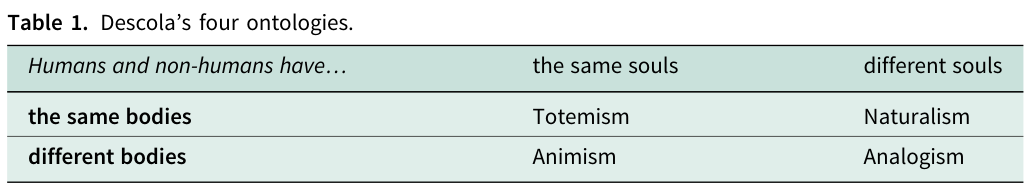
\includegraphics[width=\linewidth]{table1.png}\par
{\small 表1. 德斯科拉的四种本体论。原表文字对照：人类与非人类具有……；列为“相同的灵魂／不同的灵魂”，行为“相同的身体／不同的身体”。相同身体＋相同灵魂＝图腾主义；相同身体＋不同灵魂＝自然主义；不同身体＋相同灵魂＝泛灵论；不同身体＋不同灵魂＝类比主义。\par}\end{minipage}\end{center}
\begin{paracol}{2}
{\scriptsize\color{gray} [p. 18]}\ 乔尔·罗宾斯关于乌拉普敏基督徒道德煎熬与价值冲突的研究（Robbins 2004），以非常不同的方式体现了这一广义的形式主义家族。他对守规性与任意性的区分，明确呼应了杜蒙式结构主义的观念：成对的价值通过彼此对照来界定，并处于相互张力之中（Robbins 2013b；2015）。两个关键价值共同起作用，而且在逻辑上相互对立（如同杜蒙笔下的平等与等级），这一点并非偶然，而是罗宾斯论证架构的必要部分。因为对罗宾斯而言，如同对杜蒙而言，价值首先是\textit{关系}，其数学结构便以二的幂为基础。虽然罗宾斯不热衷交叉表，他对乌拉普敏道德生活的论述所具有的丰富复杂性与优雅，大半来自两组关系对的交叉：一组价值（任意性—守规性），以及一组语境（传统与基督教的善观念）。\par
\switchcolumn
{\scriptsize\color{gray} [p. 18]}\ Joel Robbins’ work on moral torment and value conflict amongst Urapmin Christians (Robbins 2004) exemplifies this broad family of formalisms in a very different way. Robbins’ distinction between lawfulness and willfulness harks back explicitly to a Dumontian structuralist vision of pairs of values defined and tensed against each other (Robbins 2013b; 2015). The fact that there are two key values in play, which are logically opposed (like equality and hierarchy are for Dumont), is not a contingent but an essential part of the architecture of Robbins’s argument. Since for Robbins, as for Dumont, values are first and foremost \textit{relations}, their mathematics are grounded in powers of two. While Robbins does not go in for crossed tables, much of the rich complexity and elegance of his account of Urapmin moral life comes from the intersection between two relational pairs: a pair of values (willfulness—lawfulness) and a pair of contexts (traditional and Christian visions of the good).\par
\switchcolumn*
{\scriptsize\color{gray} [p. 18]}\ 这并不是说，守规性与任意性的对立，只是一种形式手段，是人类学家自上而下强加的概念系统。对乌拉普敏人自己而言，守规性与任意性（实际上也包括基督教与传统）就是成对的对立项。如同 Ben-Yehoyada 个案中的兄弟关系／堂表亲关系，对照式配对也是一种语用手段，使乌拉普敏人能够协商并理解自己的道德世界。这正是我们所说的概念形式主义与世界中的形式之间的\textit{接口}：在交谈者的逻辑对立与人类学家的逻辑对立之间的某处，一种系统性论述生成了。在这种系统性的形式主义中，民族志与演绎逻辑携手建构这样的接口（Descola 2005b）。\par
\switchcolumn
{\scriptsize\color{gray} [p. 18]}\ This is not to say that the opposition between lawfulness and willfulness is merely a formal device, a conceptual system imposed from on high by the anthropologist. Lawfulness and willfulness (and indeed Christian and traditional) are paired opposites for the Urapmin themselves. As with the brotherhood/cousinage pair in Ben-Yehoyada’s case, contrastive pairing is also a pragmatic device that enables Urapmin to negotiate and understand their moral world. This is what we mean when we speak of an \textit{interface} between conceptual formalism and forms in the world: somewhere between the logical oppositions of interlocutors and those of the anthropologist, a systematic account arises. In this type of systematic formalism, ethnography and deductive logic work hand in hand to build such interfaces (Descola 2005b).\par
\switchcolumn*
{\scriptsize\color{gray} [p. 18]}\ 不过，以逻辑对比来建构系统，并非唯一的圈定拓扑，也不是新形式主义可以使用的唯一一种“筛子”。另一种拓扑来自形式主义的经验清单制作技术；人们可以设想继续延伸或补全这类清单。它是枚举式的，而非系统式的（例如 Luhrmann 2023）。仍以价值为题，可以在此考虑 Ori Mautner 最近的一篇文章，讨论参与集体正念冥想的以色列正统派犹太人所经历的价值冲突（2025）。Mautner 描述，在处理传统承诺与新实践之间的张力时，他的交谈者周旋于三种不同价值之间：宗教合宜性（维持“传统认可的犹太行为与观念”）、灵性（“增进自我认识，从而更亲近上帝”）以及入世性（“力求使世俗生活神圣化，而非逃离它”）。不同于守规性与任意性的对比，这些价值之间并无内在关系或逻辑张力，尽管它们在特定情境中可能发生冲突。它们也不构成一个与当前问题性质范围完全重合的系统：可以设想在论述中加入其他价值——例如对亲属的责任。相比之下，要给德斯科拉的“四大本体论”加上第五种本体论，或给罗宾斯的任意性与守规性加上第三种价值，就需要重新调整他们整个论证系统。\par
\switchcolumn
{\scriptsize\color{gray} [p. 18]}\ It is worth noting, however, that building systems out of logical contrasts is not the only topology of enclosure—not the only type of “sieve”—available to the new formalism. A different topology emerges from the formalist technique of building empirical lists that one could imagine extending or completing. It is enumerative rather than systematic (e.g., Luhrmann 2023). Staying with the theme of values, one might consider in this connection a recent article by Ori Mautner about value conflicts experienced by orthodox Israeli Jews engaging in collective mindfulness meditation (2025). In managing the tensions between traditional commitments and new practices, Mautner describes his interlocutors navigating between three different values: religious propriety (maintaining “traditionally sanctioned Jewish conduct and views”), spirituality (“developing self-acquaintance and consequently an increased intimacy with God”), and worldliness (“striving to sanctify rather than escape mundane life”). Unlike the contrast between lawfulness and willfulness, there is no inherent relationship or logical tension between these values, even though they may come into conflict in particular situations. Nor do they form a system that is coextensive with the nature of the problem at hand: one might imagine augmenting the account with other values—commitments to kin, perhaps. By contrast, to add a fifth ontology to Descola’s Big Four, or a third value to Robbins’s willfulness and lawfulness, one would need to recalibrate the entire system of their arguments.\par
\switchcolumn*
{\scriptsize\color{gray} [p. 19]}\ 这种第二类形式主义技术——制作清单——在近来对“模式”的兴趣中尤其明显，迈克尔·德加尼对此作了鲜明阐述（2024）。他借助从后社会主义舞蹈到铺装道路网络的诸多例子，说明人类学家如何描述行动者在不同形式化模式或风格之间移动；这些模式可以是身体技术、基础设施系统或伦理取向等。一位几内亚舞者在传统与即兴模式之间切换（Cohen 2016）；新几内亚的道路系统与土路小径产生不同的灵性样态和性别化具身形式（Handman 2017）；每种模式都有其约束与可能性，但行动者常常可以在保留它们独特性的同时，在其间转换。德加尼自己关于坦桑尼亚模态推理与电力基础设施的研究，也证明“模态”作为一种人类学形式所具有的生产潜力（2022；另见 Kockelman 2020）。\par
\switchcolumn
{\scriptsize\color{gray} [p. 19]}\ This second type of formalist technique—building lists—is particularly clear in the recent interest in “modes,” sharply articulated by Michael Degani (2024). Drawing on examples ranging from post-socialist dance to paved road networks, he shows how anthropologists describe actors moving between different formalized patterns or styles, whether these are, for instance, bodily techniques, infrastructural systems, or ethical orientations. A Guinean dancer shifts between traditional and improvisational modes (Cohen 2016); a road system and dirt footpaths in New Guinea produce distinct forms of spiritual modality and gendered embodiment (Handman 2017); each mode has its constraints and affordances, but actors can often shift between them while maintaining their distinctiveness. Degani’s own work on modal reasoning and electrical infrastructure in Tanzania is itself a testament to the productive potential of “modality” as an anthropological form (2022; and see Kockelman 2020).\par
\switchcolumn*
{\scriptsize\color{gray} [p. 19]}\ 这两种形式主义概念圈定技术——对照系统与开放清单——并不互相排斥：它们可以在同一论述中并用，并彼此形成张力，产生很好的效果。例如，在 Mautner 的论证中，一份可能保持开放的价值清单，又得到另一项区分的补充；这一次，是“内在”与“偶然”价值冲突之间的逻辑对立。这一区分部分地重现了我们对两种形式主义技术的区分；它本身采取逻辑对立的形式：价值冲突要么是内在的，要么是偶然的。概念圈定的形式，并不是关于世界的形而上学承诺（世界是二元的、系统性的、开放的吗？），也无需成为彼此对立的理论学派的战旗。更简单、更谦抑地说，二分法、系统、类型学与清单，只是工具——供人们使用与重新组合，以解决特定的经验和概念问题。\par
\switchcolumn
{\scriptsize\color{gray} [p. 19]}\ These two techniques of formalist conceptual enclosure—contrastive systems and open-ended lists—are not mutually exclusive: they can be deployed together and tensed against each other in the same accounts, to great effect. In Mautner’s argument, for instance, the potentially open-ended list of values is complemented by another distinction, this time a logical opposition, between “inherent” and “contingent” value conflicts. This distinction—which partly recoups our own distinction between two formalist techniques—itself takes the form of a logical opposition: value conflicts can be either inherent or they can be contingent. Forms of conceptual enclosure are not metaphysical commitments about the world (is it binary, systematic, open-ended?), nor do they need to be the battle-standards of opposing theoretical schools. Dichotomies, systems, typologies, and lists are, more simply and modestly, just tools—there to be used and recombined to solve particular empirical and conceptual problems.\par
\switchcolumn*
\end{paracol}
\Needspace{5\baselineskip}\section*{形式主义的认识德性：连贯性、可修正性与协作 / The Epistemic Virtues of Formalism: Coherence, Corrigibility, Collaboration}
\begin{paracol}{2}
{\scriptsize\color{gray} [p. 19]}\ 对比清单与结构，并不是说它们是通向形式的仅有两条路径。事实上恰恰相反：我们正在勾勒的新形式主义感受取向，独特之处正在于它对形式的多重性与多样性保持开放——无论是世界中的形式，还是我们对世界的论述中的形式。就此而言，它与反形式主义的直觉形成鲜明对照：后者认为形式是某种单一的（坏）东西，只值得以一种态度对待，即抵抗或拒绝。\par
\switchcolumn
{\scriptsize\color{gray} [p. 19]}\ In contrasting lists and structures, we are not suggesting that these are the only two pathways to form. Quite the opposite, in fact: the new formalist sensibility we are mapping is distinguished precisely by its openness to the multiplicity and diversity of forms—both in the world and in our accounts of it. In this it differs sharply from the antiformalist intuition that form is one (bad) thing, and that it only warrants a single attitude (one of resistance or refusal).\par
\switchcolumn*
{\scriptsize\color{gray} [p. 20]}\ 正如新的形式主义感受取向，并不要求对世界本性的详细本体论设定作出承诺，也不存在单一的新形式主义方法，不存在一套规定人类学分析必须（或不得）如何开展的规则手册或精确训令。我们描述的例子在主题、语调与理论取向上各不相同。它们所共享并体现的感受变化更广泛、更深刻：它涉及对某些认识德性日益增长的亲近感，而非一个精确的纲领。诉诸认识德性在人类学中并不新鲜。反形式主义也内置了自己的认识德性。在反形式主义的感受取向中，可撤回性、灵活性、开放性等，是学术研究和现实实践活动中“好”的标志，尽管本文凸显的形式主义暗流及意涵仍然存在。这里描述的新形式主义，使这些意涵及其相关德性变得明确，这恰好印证了玛丽莲·斯特拉森的观点：时代性变迁的标志往往并非新实践，而是对一直存在的实践采取了新态度。我们着重指出三种形式主义的认识德性，认为它们尤其体现当前这一新时刻的特征：连贯性、可修正性与协作。\par
\switchcolumn
{\scriptsize\color{gray} [p. 20]}\ Just as the new formalist sensibility doesn’t require a commitment to detailed ontological postulates about the nature of the world, so there is no single new formalist method, no rulebook or set of precise injunctions for how anthropological analysis must (or must not) be done. The examples we have described here differ in topic, tone, and theoretical orientation. The shift in sensibilities they share and exemplify is broader and more profound: rather than a precise program, it involves a growing affinity for certain epistemic virtues. The appeal to epistemic virtue is not new in anthropology. Antiformalism too had its own epistemic virtues built in. Revocability, flexibility, open-endedness, and the like were, in the antiformalist sensibility, the mark of the good in both scholarship and practical worldly activity, even as the formalist undercurrents and implications we have highlighted here persisted. The new formalism we describe here makes those implications and their associated virtues explicit, in an instance of Marilyn Strathern’s point that epochal change is often marked not by new practices but by new attitudes to practices that have always existed. We spotlight three formalist epistemic virtues that we feel are particularly characteristic of the current new moment: coherence, corrigibility, and collaboration.\par
\switchcolumn*
{\scriptsize\color{gray} [p. 20]}\ 人类学中的新形式主义研究，倾向于在特定论述内部形成一套连贯的概念形式。它承认，对连贯性的要求可能是一种承载权力的强加（Davé 2023），却仍珍视概念与分析工作中自我施加的连贯性：区分、范畴与术语彼此处于某种稳定关系，概念与词语从这一页到下一页大致具有相同含义。对自身连贯性的承诺，也是一种以特定方式对他人负责的承诺。在这种美学中，概念基础设施应当带有“（具有德性的）失败的可能性”（Corsín Jiménez 2014：385）。如果一种论述不可能出错，那么作为对自身之外某种事物的论述，它就价值有限，也几乎无法为集体讨论增添什么。可错性与可修正性，被视为形式主义论述中关键的、具有生产力的限制。\par
\switchcolumn
{\scriptsize\color{gray} [p. 20]}\ New formalist work in anthropology tends toward the production of a coherent set of conceptual forms within a particular account. While acknowledging that the demand for coherence can be a power-laden imposition (Davé 2023), it nevertheless values self-imposed coherence in conceptual and analytical work: distinctions, categories, terminologies that sit in some stable relation to one another, concepts and terms that mean roughly the same thing from one page to the next. This commitment to one’s own coherence is also a commitment to a certain kind of accountability to others. Conceptual infrastructures, in this aesthetic, should come with “the possibility of (virtuous) failure” (Corsín Jiménez 2014: 385). If an account cannot be wrong, it has little value as an account of something outside itself, and little to add to a collective conversation. Fallibility and corrigibility are taken as key productive limitations in formalist accounts.\par
\switchcolumn*
{\scriptsize\color{gray} [p. 20]}\ 但可修正性并不全关乎连贯性。新的人类学形式主义，还承诺在概念形式与论述之外的形式之间建立某种强关系。这种关系往往——不论人类学家愿不愿意宣扬这一事实——就是经典表征主义的对应关系。在某一层面，即便是在概念上最为精深、对老式实在论最为批判的人类学家，也仍大多在这样一个基本假设下写作：他们所说的，大体而言忠实于其民族志。我们已经看到，这种实在论精神在某些方面同样支撑着涌现与过程的美学：认为无形式的世界，必须由同样“无形式”的论述来描述（仿佛这种论述可能存在似的）。而以另一种方式，把人类学写作理解为施为性介入的反表征主义观点——将写作视为政治，无论是“本体论政治”（Mol 2002）还是其他政治——也可能同样产生富有成效的限制。如果概念形式不被看作描述，而被看作能够有效改变论述之外某种东西的工具，那么对可说之物的限制，反而可能更严格。毕竟，这种施为性的概念形式必须能够奏效。因此，除了对可错性与可修正性的承诺，我们不妨把第二种具有生产力的限制，不仅理解为“对应”，而理解为更宽泛的东西——一种“入世性”。\par
\switchcolumn
{\scriptsize\color{gray} [p. 20]}\ But corrigibility is not all about coherence. The new anthropological formalism comes with a commitment to some kind of strong relationship between conceptual forms and forms outside of the account. This relationship is often (whether anthropologists like to advertise this fact or not) one of classic representationalist correspondence. On some level, even the most conceptually sophisticated anthropological critics of old-fashioned realism still mostly write under the basic assumption that what they say is—broadly speaking—true to their ethnography. We have seen that this same spirit of realism in some ways underlies the aesthetic of emergence and process—that a world without form must be described by similarly “formless” accounts (as if such a thing were possible). And in its own way, the anti-representationalist vision of anthropological writing as performative engagement—writing as politics, “ontological” (Mol 2002) or otherwise—can be just as productively limiting. If conceptual forms are seen not as descriptions but as tools that enable an effective transformation of something beyond the account, then the limitation on what can be said is, if anything, even more stringent. For such performative conceptual forms need, after all, to work. Alongside a commitment to fallibility and to corrigibility, then, we might think of this second productive limitation not merely as “correspondence,” but as something broader—a kind of “worldliness.”\par
\switchcolumn*
{\scriptsize\color{gray} [p. 21]}\ 第三种、也许最关键的生产性限制，是向学科对话与横向的批判性交锋保持开放。Boyer 与 Howe 有力地重新构思了人类学家所谓的“理论”，指出学科内部的对话——论文报告、问答、同行评审、研究指导、合作写作等——从根本上受到一种期待的组织：知识应当能够流通。人们期待人类学论述调动一些可供其他论述使用的洞见，使其具有“\textit{跨特殊性}，成为一项与其他研究相互言说的研究……以创建沟通的路径……帮助人类学凝聚为一个独特的话语领域”（Boyer and Howe 2015）。跨特殊性不必意味着普遍性：今天鲜有人类学家会倡导那种仿照“硬科学”、建立宏大统一人类学话语的不切实际愿景。跨特殊性毋宁关乎“可携带的分析工具”（同上）——能够从一个论述流向另一个论述、被移作他用或修订后再次传递的概念形式。\par
\switchcolumn
{\scriptsize\color{gray} [p. 21]}\ A third, and perhaps, most crucial form of productive limitation is an openness to disciplinary dialogue and crosswise critical engagement. As Boyer and Howe point out in a powerful reconceptualization of what anthropologists mean by “theory,” intradisciplinary dialogue—in the form of paper-giving, Q\&As, peer review, research supervision, collaborative writing, and the like—is fundamentally structured by an expectation that knowledge should travel. An anthropological account is expected to mobilize insights that become available to other accounts, to be “\textit{transparticular}, a study that speaks with other studies … to create the communicative pathways … that help to cohere anthropology as a distinctive field of discourse” (Boyer and Howe 2015). Transparticularity need not imply universality—few anthropologists today would promote the impractical vision of a grand unified anthropological discourse modeled on the “hard sciences.” Transparticularity is rather a matter of “portable analytics” (ibid.)—conceptual forms that travel from one account to another and can be repurposed or revised and passed on again.\par
\switchcolumn*
{\scriptsize\color{gray} [p. 21]}\ 正如 Boyer 与 Howe 指出的，不承认相关前人曾尝试处理类似问题的人类学论述，往往会被批评为不够慷慨。近年，这个问题主要从“投入”的角度被讨论：当下的论述应如何建立在此前论述之上，并承认自己“取用”了什么——这既是认识问题，也是伦理与政治问题。这开启了一个广阔的争议领域：哪些先前论述应被视为相关？其中充满关于引文政治、认识正义以及经典构成的争论（Allen and Jobson 2016；Venkatesan 2025）。然而，人类学向形式的回归，对\textit{产出}问题至少给予了同等关注：每一种论述生产或改造了哪些“可携带的分析工具”，以供他人采用？这意味着，关注跨特殊性与协作，不仅要追问我们怎样合乎伦理地从彼此那里取用，也要追问怎样最好地给予。\par
\switchcolumn
{\scriptsize\color{gray} [p. 21]}\ As Boyer and Howe point out, anthropological accounts that do not acknowledge relevant previous attempts to grapple with similar problems tend to be dismissed as ungenerous. In recent years, this question has mostly been debated from the perspective of “input”: the—ethical and political as much as epistemic—question of how present accounts should build on previous ones and acknowledge what they “take.” This opens up a wide field of controversy over which previous accounts should be deemed relevant, rife with disputes over citational politics, epistemic justice, and the shape of the canon (Allen and Jobson 2016; Venkatesan 2025). The anthropological return to form, however, pays at least equal attention to the question of \textit{output}: what “portable analytics” is each account producing or refashioning for others to pick up? This means attending to transparticularity and collaboration not just as a question of how we ethically take from each other, but also as a question of how best to give.\par
\switchcolumn*
{\scriptsize\color{gray} [p. 21]}\ 由此，作为认识德性的跨特殊性／协作，又与可修正性／入世性相接。旨在共享的概念，必须经过细心制作，才能经得住其他使用者的检验——无论其内部架构，还是它与所要照亮的现象之间的外部关系，都必须如此。悖论在于，反形式主义态度之所以导致转向、新词与概念区分层出不穷，恰是因为它回避了这样的想法：这些概念可能成为稳定的协作媒介。铸造新概念，就像通过新法律，比尝试运用我们已有的概念或法律，更容易立即吸引人。如果概念不过是通往不可还原复杂性之论述道路上的必要之恶，那么，仔细关注其制作方式，或在其任务结束后继续保留它们，就没有多大收益。每一种个别论述都可以发起自己的概念革命，然后继续前行。相比之下，新的形式主义美学关注概念再利用的实际运作。好工具值得磨利和修补——而且可以出借，也可以借用。\par
\switchcolumn
{\scriptsize\color{gray} [p. 21]}\ In this connection, transparticularity/collaboration as an epistemic virtue rejoins corrigibility/worldliness. Concepts designed to be shared have to be carefully crafted to stand the test of other users––both in their internal architecture and in their external relation to the phenomena they purport to illuminate. Paradoxically, the antiformalist attitude has led to a proliferation of turns, neologisms, and conceptual distinctions, precisely because it eschewed the thought that these concepts might become stable tokens of collaboration. Coining new concepts, like passing new laws, is more immediately appealing than trying to apply the ones we already have. If concepts are just necessary evils on the path to an account of irreducible complexity, then there is little mileage in paying much attention to how they are crafted or in keeping them around after their work is done. Each individual account can provide its own conceptual revolution, and move on. The new formalist aesthetic, by contrast, keeps an eye on the pragmatics of conceptual reuse. Good tools are worth sharpening and fixing—one can lend and borrow them, too.\par
\switchcolumn*
\end{paracol}
\Needspace{5\baselineskip}\section*{结论：接下来是什么？ / Conclusion: What Comes Next?}
\begin{paracol}{2}
{\scriptsize\color{gray} [p. 21]}\ 因此，我们所谓的新形式主义感受取向，由两个成分构成：关注世界中的规律性并为之困惑，以及致力于围绕这些规律性制作概念圈定。它们并非相互独立的举措：世界中的规律性，常常只有与我们的概念形式主义相遇时才变得可见。与（其他）科学对象一样，模式、价值、文化、潮流、角色、技术、亲属结构等，都是混合产物：它们产生于一种概念工具与世界中某种能够反过来“提出异议”的事物之间的成功衔接（Stengers 2000）。按我们的理解，人类学形式主义要求概念形式与世界的规律性之间存在某种接口。这不仅是“赋予民族志现象特定的概念形状”（Holbraad 2020），还包括允许现象自身的形状扭曲、引导并反对我们的概念形式主义之形状。Kingston（2003）在一次早期而深刻的、呼吁人类学回归形式的论述中指出，形式与注意具有内在联系：“形式本身只有在与无形式的关系中才存在，正如专注的区域相对于不留意而存在”（同上：685）。概念形式主义在其最佳状态下，表现为对某种特定关注方式的重新承诺。\par
\switchcolumn
{\scriptsize\color{gray} [p. 21]}\ The two ingredients of what we are calling a new formalist sensibility, then, are an attention to and puzzling over regularities in the world, and a commitment to crafting conceptual enclosures around them. These are not independent moves: regularities in the world often only become visible as they meet with our conceptual formalisms. Like (other) scientific objects, modes, values, cultures, trends, roles, techniques, kinship structures, and so forth are hybrids: they are the result of a successful articulation between a conceptual device and something in the world that “objects” back (Stengers 2000). Anthropological formalism as we conceive it requires some interface between conceptual forms and worldly regularities. This is not just a matter of “giving ethnographic phenomena particular conceptual shapes” (Holbraad 2020), but also of allowing the shape of phenomena to distort, guide, and object to the shape of our conceptual formalisms. Form—as Kingston (2003) observed in an early and profound call for a return to form in anthropology—is inherently related to attention: “Form itself only exists in relation to the formless, as areas of focused attention are relative to inattentiveness” (ibid.: 685). Conceptual formalisms, at their best, manifest a renewed commitment to a particular kind of attentiveness.\par
\switchcolumn*
{\scriptsize\color{gray} [p. 22]}\ 但这种关注也应延伸至形式／反形式的整体动态。如果当代人类学中的形式主义美学确实显得势头渐盛，这一动力部分来自它借旧有反形式主义共识作为支点向外推开——形式只能在与无形式的关系中存在。这本身既不值得庆祝，也无须惋惜；学科热情就是这样从对立中获得驱动力的。它只是提醒那些像我们一样为新形式主义美学所鼓舞的人：不妨持续追问，我们仍然珍视并运用哪些反形式主义？从那个正迅速显得已成历史的反形式主义人类学时刻中，有什么值得保留？\par
\switchcolumn
{\scriptsize\color{gray} [p. 22]}\ Yet this attention should extend also to the form/antiform dynamic as a whole. Insofar as a formalist aesthetic feels like it has momentum in contemporary anthropology, this momentum comes in part from pushing off from an older antiformalist consensus—form can only exist in relation to the formless. This is not in itself something to be either celebrated or regretted—it is the way of disciplinary enthusiasms, to get their drive from opposition. It simply reminds those who—like us—are enthused by the new formalist aesthetic that we may do well to keep asking what antiformalisms we still nevertheless value and deploy, and what is worth retaining from the antiformalist anthropological moment that is rapidly coming to feel historical.\par
\switchcolumn*
{\scriptsize\color{gray} [p. 22]}\ 开篇所描述的反形式主义美学，以无数方式帮助了人类学。其中尤为重要的是，它先帮助拆解、随后又帮助防范那些过度僵硬的结构模型卷土重来，因为这些模型可能压平民族志的复杂性。但现在已是不同的历史时刻，学科（以及世界）面临的威胁也有所不同。大型语言模型激发了公众对模式识别以及形式与意义之间更广泛关系的兴趣与争论。各种政治动员，一方面要求承认某些稳定的类别身份，另一方面又坚持消解另一些类别身份。欧美的经济与职业生活，日益充斥着对管理主义、官僚制和问责的关切。与此同时，如前所述，大众话语越来越多地运用反形式主义修辞，赞颂破坏、拒绝专业知识与制度约束；但其目的，却使反形式主义那些曾经明显具有进步性的姿态，如今显得令人担忧。\par
\switchcolumn
{\scriptsize\color{gray} [p. 22]}\ The antiformalist aesthetic we began by describing served anthropology in innumerable ways, not least by helping first to dismantle and then to guard against the return of overly rigid structural models that threatened to flatten ethnographic complexity. This, though, is a different historical moment, and the threats the discipline (and the world) face are different too. Large language models have sparked public interest and debate about pattern recognition and the wider relationship between form and meaning. Political mobilizations of various types demand recognition of some stable categorical identities whilst insisting on the dissolution of others. Economic and professional life in Euro-America is increasingly suffused by concerns about managerialism, bureaucracy, and accountability. Meanwhile, as we have noted, popular discourse has seen the increasing deployment of antiformalist rhetoric in celebration of disruption and the rejection of expertise and institutional constraints, but toward ends that make antiformalism’s once clearly progressive gestures look newly concerning.\par
\switchcolumn*
{\scriptsize\color{gray} [p. 22]}\ 因此，我们试图辨认的新形式主义美学，并非源于对昔日确定性的怀旧，而源于一种信念：人类学能够制作理论、论证与模型，对当代世界的复杂性说出独特的东西。形式化与反形式化的举措将继续在人类学研究中相互交织，这种往复摆动植根于学科的本性。但这种摆动所包含的，不只是思想时尚或潮流。理论学派与转向可能来去不定，而今天形式的兴起，如同二十世纪八十年代实践的兴起，指向更具时代意义的变化，并回应着根本性的知识与现实挑战。\par
\switchcolumn
{\scriptsize\color{gray} [p. 22]}\ So the new formalist aesthetic we have sought to identify does not emerge from a nostalgia for past certainties, but from a belief in anthropology’s capacity to craft theories, arguments, and models that say something distinctive about the contemporary world’s complexity. Formal and anti-formal moves will continue to intertwine in anthropological work, and that oscillation is baked into the nature of the discipline. But there is more to such oscillation than mere intellectual fads or trends. Theoretical schools and turns might come and go, but the rise of form today, like that of practice in the 1980s, points to something more epochal and addresses fundamental intellectual and worldly challenges.\par
\switchcolumn*
\end{paracol}
\Needspace{5\baselineskip}\section*{致谢 / Acknowledgements}
\begin{paracol}{2}
{\scriptsize\color{gray} [p. 22]}\ 作者感谢 Naor Ben-Yehoyada、Joanna Cook、Mike Degani、James Laidlaw、Adam Reed、Andrew Shryock、Marilyn Strathern 与 Tom Yarrow 对本文早期稿件提出深思熟虑的意见。也感谢 Jatin Dua、Lauren Kapsalakis 及四位匿名评审，在修改本文以供《社会与历史比较研究》（CSSH）发表的过程中给予慷慨帮助。\par
\switchcolumn
{\scriptsize\color{gray} [p. 22]}\ The authors would like to thank Naor Ben-Yehoyada, Joanna Cook, Mike Degani, James Laidlaw, Adam Reed, Andrew Shryock, Marilyn Strathern, and Tom Yarrow for their very thoughtful views on earlier drafts of this paper. We are also grateful to Jatin Dua, Lauren Kapsalakis, and to four anonymous reviewers for their generous help in revising the paper for publication in CSSH.\par
\switchcolumn*
\end{paracol}
\Needspace{5\baselineskip}\section*{参考文献 / References}
\noindent\begin{minipage}{\textwidth}\begin{minipage}[t]{\dimexpr.5\textwidth-4mm\relax}\noindent\begin{minipage}[t]{\linewidth}{\scriptsize\color{gray} [p. 23]}\ Agha, A. 2006. Language and Social Relations. Leiden: Cambridge University Press. At: \url{http://public.eblib.com/choice/publicfullrecord.aspx?p=279321,} accessed 21 December 2016. DOI: \url{10.1017/CBO9780511618284} 〔题名译释：语言与社会关系。〕\par\end{minipage}\par\end{minipage}\hfill\begin{minipage}[t]{\dimexpr.5\textwidth-4mm\relax}\noindent\begin{minipage}[t]{\linewidth}{\scriptsize\color{gray} [p. 23]}\ Agha, A. 2006. Language and Social Relations. Leiden: Cambridge University Press. At: \url{http://public.eblib.com/choice/publicfullrecord.aspx?p=279321,} accessed 21 December 2016. DOI: \url{10.1017/CBO9780511618284}\par\end{minipage}\par\end{minipage}\end{minipage}\par
\noindent\begin{minipage}{\textwidth}\begin{minipage}[t]{\dimexpr.5\textwidth-4mm\relax}\noindent\begin{minipage}[t]{\linewidth}{\scriptsize\color{gray} [p. 23]}\ Albris, K., Candea, M., Enggard, T., Jakobsen, T., and Pedersen, M.. 2025. Measuring MAN (incorporating JRAI): Computational Anthropological Analysis and Quantitative Speculation. Journal of the Royal Anthropological Institute 32 (July): 32–54. DOI: \url{10.1111/1467-9655.14290} 〔题名译释：测量《MAN》（并入《JRAI》）：计算人类学分析与定量推想。〕\par\end{minipage}\par\end{minipage}\hfill\begin{minipage}[t]{\dimexpr.5\textwidth-4mm\relax}\noindent\begin{minipage}[t]{\linewidth}{\scriptsize\color{gray} [p. 23]}\ Albris, K., Candea, M., Enggard, T., Jakobsen, T., and Pedersen, M.. 2025. Measuring MAN (incorporating JRAI): Computational Anthropological Analysis and Quantitative Speculation. Journal of the Royal Anthropological Institute 32 (July): 32–54. DOI: \url{10.1111/1467-9655.14290}\par\end{minipage}\par\end{minipage}\end{minipage}\par
\noindent\begin{minipage}{\textwidth}\begin{minipage}[t]{\dimexpr.5\textwidth-4mm\relax}\noindent\begin{minipage}[t]{\linewidth}{\scriptsize\color{gray} [p. 23]}\ Alexander, C. 2017. The Meeting as Subjunctive Form: Public/Private IT Projects in British and Turkish State Bureaucracies. Journal of the Royal Anthropological Institute 23, S1: 80–94. DOI: \url{10.1111/1467-9655.12595} 〔题名译释：作为虚拟式形式的会议：英国与土耳其国家官僚体系中的公私信息技术项目。〕\par\end{minipage}\par\end{minipage}\hfill\begin{minipage}[t]{\dimexpr.5\textwidth-4mm\relax}\noindent\begin{minipage}[t]{\linewidth}{\scriptsize\color{gray} [p. 23]}\ Alexander, C. 2017. The Meeting as Subjunctive Form: Public/Private IT Projects in British and Turkish State Bureaucracies. Journal of the Royal Anthropological Institute 23, S1: 80–94. DOI: \url{10.1111/1467-9655.12595}\par\end{minipage}\par\end{minipage}\end{minipage}\par
\noindent\begin{minipage}{\textwidth}\begin{minipage}[t]{\dimexpr.5\textwidth-4mm\relax}\noindent\begin{minipage}[t]{\linewidth}{\scriptsize\color{gray} [p. 23]}\ Allen, J. S. and Jobson, R. C. 2016. The Decolonizing Generation: (Race and) Theory in Anthropology Since the Eighties. Current Anthropology 57, 2: 129–148. DOI: \url{10.1086/685502} 〔题名译释：去殖民化的一代：八十年代以来人类学中的（种族与）理论。〕\par\end{minipage}\par\end{minipage}\hfill\begin{minipage}[t]{\dimexpr.5\textwidth-4mm\relax}\noindent\begin{minipage}[t]{\linewidth}{\scriptsize\color{gray} [p. 23]}\ Allen, J. S. and Jobson, R. C. 2016. The Decolonizing Generation: (Race and) Theory in Anthropology Since the Eighties. Current Anthropology 57, 2: 129–148. DOI: \url{10.1086/685502}\par\end{minipage}\par\end{minipage}\end{minipage}\par
\noindent\begin{minipage}{\textwidth}\begin{minipage}[t]{\dimexpr.5\textwidth-4mm\relax}\noindent\begin{minipage}[t]{\linewidth}{\scriptsize\color{gray} [p. 23]}\ Asad, T. 2003. Formations of the Secular: Christianity, Islam, Modernity. Stanford: Stanford University Press. 〔题名译释：世俗的构型：基督教、伊斯兰与现代性。〕\par\end{minipage}\par\end{minipage}\hfill\begin{minipage}[t]{\dimexpr.5\textwidth-4mm\relax}\noindent\begin{minipage}[t]{\linewidth}{\scriptsize\color{gray} [p. 23]}\ Asad, T. 2003. Formations of the Secular: Christianity, Islam, Modernity. Stanford: Stanford University Press.\par\end{minipage}\par\end{minipage}\end{minipage}\par
\noindent\begin{minipage}{\textwidth}\begin{minipage}[t]{\dimexpr.5\textwidth-4mm\relax}\noindent\begin{minipage}[t]{\linewidth}{\scriptsize\color{gray} [p. 23]}\ Bandak, A. 2015. Exemplary Series and Christian Typology: Modelling on Sainthood in Damascus. Journal of the Royal Anthropological Institute. 21, S1: 47–63. DOI: \url{10.1111/1467-9655.12165} 〔题名译释：典范系列与基督教预型论：大马士革以圣徒性为范式的实践。〕\par\end{minipage}\par\end{minipage}\hfill\begin{minipage}[t]{\dimexpr.5\textwidth-4mm\relax}\noindent\begin{minipage}[t]{\linewidth}{\scriptsize\color{gray} [p. 23]}\ Bandak, A. 2015. Exemplary Series and Christian Typology: Modelling on Sainthood in Damascus. Journal of the Royal Anthropological Institute. 21, S1: 47–63. DOI: \url{10.1111/1467-9655.12165}\par\end{minipage}\par\end{minipage}\end{minipage}\par
\noindent\begin{minipage}{\textwidth}\begin{minipage}[t]{\dimexpr.5\textwidth-4mm\relax}\noindent\begin{minipage}[t]{\linewidth}{\scriptsize\color{gray} [p. 23]}\ Barad, K. M. 2007. Meeting the Universe Halfway: Quantum Physics and the Entanglement of Matter and Meaning. Durham: Duke University Press. DOI: \url{10.2307/j.ctv12101zq} 〔题名译释：与宇宙相遇于半途：量子物理学以及物质与意义的纠缠。〕\par\end{minipage}\par\end{minipage}\hfill\begin{minipage}[t]{\dimexpr.5\textwidth-4mm\relax}\noindent\begin{minipage}[t]{\linewidth}{\scriptsize\color{gray} [p. 23]}\ Barad, K. M. 2007. Meeting the Universe Halfway: Quantum Physics and the Entanglement of Matter and Meaning. Durham: Duke University Press. DOI: \url{10.2307/j.ctv12101zq}\par\end{minipage}\par\end{minipage}\end{minipage}\par
\noindent\begin{minipage}{\textwidth}\begin{minipage}[t]{\dimexpr.5\textwidth-4mm\relax}\noindent\begin{minipage}[t]{\linewidth}{\scriptsize\color{gray} [p. 23]}\ Bear, L., Ho, K., Tsing, A. L., and Yanagisako., S. 2015. Gens: A Feminist Manifesto for the Study of Capitalism. Society for Cultural Anthropology. \url{https://culanth.org.} 〔题名译释：Gens：研究资本主义的女性主义宣言。〕\par\end{minipage}\par\end{minipage}\hfill\begin{minipage}[t]{\dimexpr.5\textwidth-4mm\relax}\noindent\begin{minipage}[t]{\linewidth}{\scriptsize\color{gray} [p. 23]}\ Bear, L., Ho, K., Tsing, A. L., and Yanagisako., S. 2015. Gens: A Feminist Manifesto for the Study of Capitalism. Society for Cultural Anthropology. \url{https://culanth.org.}\par\end{minipage}\par\end{minipage}\end{minipage}\par
\noindent\begin{minipage}{\textwidth}\begin{minipage}[t]{\dimexpr.5\textwidth-4mm\relax}\noindent\begin{minipage}[t]{\linewidth}{\scriptsize\color{gray} [p. 23]}\ Ben-Yehoyada, N. 2014. Transnational Political Cosmology: A Central Mediterranean Example. Comparative Studies in Society and History 56, 4: 870–901. DOI: \url{10.1017/S0010417514000437} 〔题名译释：跨国政治宇宙论：地中海中部的一个例子。〕\par\end{minipage}\par\end{minipage}\hfill\begin{minipage}[t]{\dimexpr.5\textwidth-4mm\relax}\noindent\begin{minipage}[t]{\linewidth}{\scriptsize\color{gray} [p. 23]}\ Ben-Yehoyada, N. 2014. Transnational Political Cosmology: A Central Mediterranean Example. Comparative Studies in Society and History 56, 4: 870–901. DOI: \url{10.1017/S0010417514000437}\par\end{minipage}\par\end{minipage}\end{minipage}\par
\noindent\begin{minipage}{\textwidth}\begin{minipage}[t]{\dimexpr.5\textwidth-4mm\relax}\noindent\begin{minipage}[t]{\linewidth}{\scriptsize\color{gray} [p. 23]}\ Biehl, J. and Locke, P.. 2010. Deleuze and the Anthropology of Becoming. Current Anthropology 51, 3: 317–51. DOI: \url{10.1086/651466} 〔题名译释：德勒兹与生成的人类学。〕\par\end{minipage}\par\end{minipage}\hfill\begin{minipage}[t]{\dimexpr.5\textwidth-4mm\relax}\noindent\begin{minipage}[t]{\linewidth}{\scriptsize\color{gray} [p. 23]}\ Biehl, J. and Locke, P.. 2010. Deleuze and the Anthropology of Becoming. Current Anthropology 51, 3: 317–51. DOI: \url{10.1086/651466}\par\end{minipage}\par\end{minipage}\end{minipage}\par
\noindent\begin{minipage}{\textwidth}\begin{minipage}[t]{\dimexpr.5\textwidth-4mm\relax}\noindent\begin{minipage}[t]{\linewidth}{\scriptsize\color{gray} [p. 23]}\ Boellstorff, T. 2010. A Typology of Ethnographic Scales for Virtual Worlds. In Bainbridge, W. S., ed., Online Worlds: Convergence of the Real and the Virtual. London: Springer London, 123–33. DOI: \url{10.1007/978-1-84882-825-4_10} 〔题名译释：虚拟世界民族志尺度的类型学；所收文集：在线世界：真实与虚拟的汇合。〕\par\end{minipage}\par\end{minipage}\hfill\begin{minipage}[t]{\dimexpr.5\textwidth-4mm\relax}\noindent\begin{minipage}[t]{\linewidth}{\scriptsize\color{gray} [p. 23]}\ Boellstorff, T. 2010. A Typology of Ethnographic Scales for Virtual Worlds. In Bainbridge, W. S., ed., Online Worlds: Convergence of the Real and the Virtual. London: Springer London, 123–33. DOI: \url{10.1007/978-1-84882-825-4_10}\par\end{minipage}\par\end{minipage}\end{minipage}\par
\noindent\begin{minipage}{\textwidth}\begin{minipage}[t]{\dimexpr.5\textwidth-4mm\relax}\noindent\begin{minipage}[t]{\linewidth}{\scriptsize\color{gray} [p. 23]}\ Bourdieu, P. 1977. Outline of a Theory of Practice. Cambridge: Cambridge University Press. DOI: \url{10.1017/CBO9780511812507} 〔题名译释：实践理论大纲。〕\par\end{minipage}\par\end{minipage}\hfill\begin{minipage}[t]{\dimexpr.5\textwidth-4mm\relax}\noindent\begin{minipage}[t]{\linewidth}{\scriptsize\color{gray} [p. 23]}\ Bourdieu, P. 1977. Outline of a Theory of Practice. Cambridge: Cambridge University Press. DOI: \url{10.1017/CBO9780511812507}\par\end{minipage}\par\end{minipage}\end{minipage}\par
\noindent\begin{minipage}{\textwidth}\begin{minipage}[t]{\dimexpr.5\textwidth-4mm\relax}\noindent\begin{minipage}[t]{\linewidth}{\scriptsize\color{gray} [p. 23]}\ Boyer, D. 2013. Simply the Best: Parody and Political Sincerity in Iceland. American Ethnologist. 40, 2: 276–87. DOI: \url{10.1111/amet.12020} 〔题名译释：简直最好：冰岛的戏仿与政治真诚。〕\par\end{minipage}\par\end{minipage}\hfill\begin{minipage}[t]{\dimexpr.5\textwidth-4mm\relax}\noindent\begin{minipage}[t]{\linewidth}{\scriptsize\color{gray} [p. 23]}\ Boyer, D. 2013. Simply the Best: Parody and Political Sincerity in Iceland. American Ethnologist. 40, 2: 276–87. DOI: \url{10.1111/amet.12020}\par\end{minipage}\par\end{minipage}\end{minipage}\par
\noindent\begin{minipage}{\textwidth}\begin{minipage}[t]{\dimexpr.5\textwidth-4mm\relax}\noindent\begin{minipage}[t]{\linewidth}{\scriptsize\color{gray} [p. 23]}\ Boyer, D. and Howe, C.. 2015. Portable Analytics and Lateral Theory. In Boyer, D., Faubion, J., and Marcus, G., eds., Theory Can Be More than It Used to Be: Learning Anthropology’s Method in a Time of Transition. Ithaca: Cornell University Press, 15–38. 〔题名译释：可携带的分析工具与横向理论；所收文集：理论可以超越往昔：在转型时期学习人类学方法。〕\par\end{minipage}\par\end{minipage}\hfill\begin{minipage}[t]{\dimexpr.5\textwidth-4mm\relax}\noindent\begin{minipage}[t]{\linewidth}{\scriptsize\color{gray} [p. 23]}\ Boyer, D. and Howe, C.. 2015. Portable Analytics and Lateral Theory. In Boyer, D., Faubion, J., and Marcus, G., eds., Theory Can Be More than It Used to Be: Learning Anthropology’s Method in a Time of Transition. Ithaca: Cornell University Press, 15–38.\par\end{minipage}\par\end{minipage}\end{minipage}\par
\noindent\begin{minipage}{\textwidth}\begin{minipage}[t]{\dimexpr.5\textwidth-4mm\relax}\noindent\begin{minipage}[t]{\linewidth}{\scriptsize\color{gray} [p. 23]}\ Boyer, D. and Yurchak, A.. 2010. American Stiob: Or, What Late-Socialist Aesthetics of Parody Reveal about Contemporary Political Culture in the West. Cultural Anthropology 25, 2: 179–221. DOI: \url{10.1111/j.1548-1360.2010.01056.x} 〔题名译释：美国式 Stiob：或者，晚期社会主义的戏仿美学揭示了当代西方政治文化的什么。〕\par\end{minipage}\par\end{minipage}\hfill\begin{minipage}[t]{\dimexpr.5\textwidth-4mm\relax}\noindent\begin{minipage}[t]{\linewidth}{\scriptsize\color{gray} [p. 23]}\ Boyer, D. and Yurchak, A.. 2010. American Stiob: Or, What Late-Socialist Aesthetics of Parody Reveal about Contemporary Political Culture in the West. Cultural Anthropology 25, 2: 179–221. DOI: \url{10.1111/j.1548-1360.2010.01056.x}\par\end{minipage}\par\end{minipage}\end{minipage}\par
\noindent\begin{minipage}{\textwidth}\begin{minipage}[t]{\dimexpr.5\textwidth-4mm\relax}\noindent\begin{minipage}[t]{\linewidth}{\scriptsize\color{gray} [p. 23]}\ Bunzl, M. 2008. The Quest for Anthropological Relevance: Borgesian Maps and Epistemological Pitfalls. American Anthropologist 110, 1: 53–60. DOI: \url{10.1111/j.1548-1433.2008.00008.x} 〔题名译释：追寻人类学的相关性：博尔赫斯式地图与认识论陷阱。〕\par\end{minipage}\par\end{minipage}\hfill\begin{minipage}[t]{\dimexpr.5\textwidth-4mm\relax}\noindent\begin{minipage}[t]{\linewidth}{\scriptsize\color{gray} [p. 23]}\ Bunzl, M. 2008. The Quest for Anthropological Relevance: Borgesian Maps and Epistemological Pitfalls. American Anthropologist 110, 1: 53–60. DOI: \url{10.1111/j.1548-1433.2008.00008.x}\par\end{minipage}\par\end{minipage}\end{minipage}\par
\noindent\begin{minipage}{\textwidth}\begin{minipage}[t]{\dimexpr.5\textwidth-4mm\relax}\noindent\begin{minipage}[t]{\linewidth}{\scriptsize\color{gray} [p. 23]}\ Candea, M. 2007. Arbitrary Locations: In Defence of the Bounded Field-Site. Journal of the Royal Anthropological Institute 13, 1: 167–84. DOI: \url{10.1111/j.1467-9655.2007.00419.x} 〔题名译释：任意的地点：为有界的田野地点辩护。〕\par\end{minipage}\par\end{minipage}\hfill\begin{minipage}[t]{\dimexpr.5\textwidth-4mm\relax}\noindent\begin{minipage}[t]{\linewidth}{\scriptsize\color{gray} [p. 23]}\ Candea, M. 2007. Arbitrary Locations: In Defence of the Bounded Field-Site. Journal of the Royal Anthropological Institute 13, 1: 167–84. DOI: \url{10.1111/j.1467-9655.2007.00419.x}\par\end{minipage}\par\end{minipage}\end{minipage}\par
\noindent\begin{minipage}{\textwidth}\begin{minipage}[t]{\dimexpr.5\textwidth-4mm\relax}\noindent\begin{minipage}[t]{\linewidth}{\scriptsize\color{gray} [p. 23]}\ Candea, M. 2016. We Have Never Been Pluralist: On Lateral and Frontal Comparisons in the Ontological Turn. In Charbonnier, P., Salmon, G., and Skafish, P., eds., Comparative Metaphysics: Ontology after Anthropology. London: Rowman \& Littlefield, 85–106. DOI: \url{10.5040/9798881812645.ch-4} 〔题名译释：我们从未是多元论者：论本体论转向中的横向比较与正面比较；所收文集：比较形而上学：人类学之后的本体论。〕\par\end{minipage}\par\end{minipage}\hfill\begin{minipage}[t]{\dimexpr.5\textwidth-4mm\relax}\noindent\begin{minipage}[t]{\linewidth}{\scriptsize\color{gray} [p. 23]}\ Candea, M. 2016. We Have Never Been Pluralist: On Lateral and Frontal Comparisons in the Ontological Turn. In Charbonnier, P., Salmon, G., and Skafish, P., eds., Comparative Metaphysics: Ontology after Anthropology. London: Rowman \& Littlefield, 85–106. DOI: \url{10.5040/9798881812645.ch-4}\par\end{minipage}\par\end{minipage}\end{minipage}\par
\noindent\begin{minipage}{\textwidth}\begin{minipage}[t]{\dimexpr.5\textwidth-4mm\relax}\noindent\begin{minipage}[t]{\linewidth}{\scriptsize\color{gray} [p. 23]}\ Candea, M. 2019. Comparison in Anthropology: The Impossible Method. Cambridge: Cambridge University Press. 〔题名译释：人类学中的比较：不可能的方法。〕\par\end{minipage}\par\end{minipage}\hfill\begin{minipage}[t]{\dimexpr.5\textwidth-4mm\relax}\noindent\begin{minipage}[t]{\linewidth}{\scriptsize\color{gray} [p. 23]}\ Candea, M. 2019. Comparison in Anthropology: The Impossible Method. Cambridge: Cambridge University Press.\par\end{minipage}\par\end{minipage}\end{minipage}\par
\noindent\begin{minipage}{\textwidth}\begin{minipage}[t]{\dimexpr.5\textwidth-4mm\relax}\noindent\begin{minipage}[t]{\linewidth}{\scriptsize\color{gray} [p. 23]}\ Candea, M. 2025. A Return to Form. Social Analysis 69, 1. DOI: \url{10.3167/sa.2025.690103} 〔题名译释：回归形式。〕\par\end{minipage}\par\end{minipage}\hfill\begin{minipage}[t]{\dimexpr.5\textwidth-4mm\relax}\noindent\begin{minipage}[t]{\linewidth}{\scriptsize\color{gray} [p. 23]}\ Candea, M. 2025. A Return to Form. Social Analysis 69, 1. DOI: \url{10.3167/sa.2025.690103}\par\end{minipage}\par\end{minipage}\end{minipage}\par
\noindent\begin{minipage}{\textwidth}\begin{minipage}[t]{\dimexpr.5\textwidth-4mm\relax}\noindent\begin{minipage}[t]{\linewidth}{\scriptsize\color{gray} [p. 23]}\ Clarke, M. 2015. Legalism and the Care of the Self: Sharīʿah Discourse in Contemporary Lebanon. In Dresch, P. and Scheele, J., eds., Legalism: Rules and Categories. Oxford Scholarship Online, 231–57. DOI: \url{10.1093/acprof:oso/9780198753810.003.0010} 〔题名译释：律法主义与自我的关怀：当代黎巴嫩的沙里亚话语；所收文集：律法主义：规则与范畴。〕\par\end{minipage}\par\end{minipage}\hfill\begin{minipage}[t]{\dimexpr.5\textwidth-4mm\relax}\noindent\begin{minipage}[t]{\linewidth}{\scriptsize\color{gray} [p. 23]}\ Clarke, M. 2015. Legalism and the Care of the Self: Sharīʿah Discourse in Contemporary Lebanon. In Dresch, P. and Scheele, J., eds., Legalism: Rules and Categories. Oxford Scholarship Online, 231–57. DOI: \url{10.1093/acprof:oso/9780198753810.003.0010}\par\end{minipage}\par\end{minipage}\end{minipage}\par
\noindent\begin{minipage}{\textwidth}\begin{minipage}[t]{\dimexpr.5\textwidth-4mm\relax}\noindent\begin{minipage}[t]{\linewidth}{\scriptsize\color{gray} [p. 23]}\ Clifford, J. 1981. On Ethnographic Surrealism. Comparative Studies in Society and History 23, 4: 539–64. DOI: \url{10.1017/S0010417500013554} 〔题名译释：论民族志的超现实主义。〕\par\end{minipage}\par\end{minipage}\hfill\begin{minipage}[t]{\dimexpr.5\textwidth-4mm\relax}\noindent\begin{minipage}[t]{\linewidth}{\scriptsize\color{gray} [p. 23]}\ Clifford, J. 1981. On Ethnographic Surrealism. Comparative Studies in Society and History 23, 4: 539–64. DOI: \url{10.1017/S0010417500013554}\par\end{minipage}\par\end{minipage}\end{minipage}\par
\noindent\begin{minipage}{\textwidth}\begin{minipage}[t]{\dimexpr.5\textwidth-4mm\relax}\noindent\begin{minipage}[t]{\linewidth}{\scriptsize\color{gray} [p. 23]}\ Cohen, A. 2016. Inalienable Performances, Mutable Heirlooms: Dance, Cultural Inheritance, and Political Transformation in the Republic of Guinea. American Ethnologist 43, 4: 650–62. DOI: \url{10.1111/amet.12381} 〔题名译释：不可让渡的表演、可变的传家之物：几内亚共和国的舞蹈、文化继承与政治转型。〕\par\end{minipage}\par\end{minipage}\hfill\begin{minipage}[t]{\dimexpr.5\textwidth-4mm\relax}\noindent\begin{minipage}[t]{\linewidth}{\scriptsize\color{gray} [p. 23]}\ Cohen, A. 2016. Inalienable Performances, Mutable Heirlooms: Dance, Cultural Inheritance, and Political Transformation in the Republic of Guinea. American Ethnologist 43, 4: 650–62. DOI: \url{10.1111/amet.12381}\par\end{minipage}\par\end{minipage}\end{minipage}\par
\noindent\begin{minipage}{\textwidth}\begin{minipage}[t]{\dimexpr.5\textwidth-4mm\relax}\noindent\begin{minipage}[t]{\linewidth}{\scriptsize\color{gray} [p. 23]}\ Coole, D. and Frost, S.. 2010. New Materialisms: Ontology, Agency, and Politics. Durham: Duke University Press. 〔题名译释：新唯物主义：本体论、能动性与政治。〕\par\end{minipage}\par\end{minipage}\hfill\begin{minipage}[t]{\dimexpr.5\textwidth-4mm\relax}\noindent\begin{minipage}[t]{\linewidth}{\scriptsize\color{gray} [p. 23]}\ Coole, D. and Frost, S.. 2010. New Materialisms: Ontology, Agency, and Politics. Durham: Duke University Press.\par\end{minipage}\par\end{minipage}\end{minipage}\par
\noindent\begin{minipage}{\textwidth}\begin{minipage}[t]{\dimexpr.5\textwidth-4mm\relax}\noindent\begin{minipage}[t]{\linewidth}{\scriptsize\color{gray} [p. 23]}\ Corsín Jiménez, A. 2014. Introduction: The Prototype: More than Many and Less than One. Journal of Cultural Economy. 7, 4: 381–98. DOI: \url{10.1080/17530350.2013.858059} 〔题名译释：导论：原型——多于多、少于一。〕\par\end{minipage}\par\end{minipage}\hfill\begin{minipage}[t]{\dimexpr.5\textwidth-4mm\relax}\noindent\begin{minipage}[t]{\linewidth}{\scriptsize\color{gray} [p. 23]}\ Corsín Jiménez, A. 2014. Introduction: The Prototype: More than Many and Less than One. Journal of Cultural Economy. 7, 4: 381–98. DOI: \url{10.1080/17530350.2013.858059}\par\end{minipage}\par\end{minipage}\end{minipage}\par
\noindent\begin{minipage}{\textwidth}\begin{minipage}[t]{\dimexpr.5\textwidth-4mm\relax}\noindent\begin{minipage}[t]{\linewidth}{\scriptsize\color{gray} [p. 23]}\ Culler, J. 2018. 1980: Structuralism and Poststructuralism. Ex-position 40: 79–94. 〔题名译释：1980：结构主义与后结构主义。〕\par\end{minipage}\par\end{minipage}\hfill\begin{minipage}[t]{\dimexpr.5\textwidth-4mm\relax}\noindent\begin{minipage}[t]{\linewidth}{\scriptsize\color{gray} [p. 23]}\ Culler, J. 2018. 1980: Structuralism and Poststructuralism. Ex-position 40: 79–94.\par\end{minipage}\par\end{minipage}\end{minipage}\par
\noindent\begin{minipage}{\textwidth}\begin{minipage}[t]{\dimexpr.5\textwidth-4mm\relax}\noindent\begin{minipage}[t]{\linewidth}{\scriptsize\color{gray} [p. 24]}\ Davé, N. N. 2023. Indifference: On the Praxis of Interspecies Being. Duke University Press Books. 〔题名译释：无差别：论跨物种存在的实践。〕\par\end{minipage}\par\end{minipage}\hfill\begin{minipage}[t]{\dimexpr.5\textwidth-4mm\relax}\noindent\begin{minipage}[t]{\linewidth}{\scriptsize\color{gray} [p. 24]}\ Davé, N. N. 2023. Indifference: On the Praxis of Interspecies Being. Duke University Press Books.\par\end{minipage}\par\end{minipage}\end{minipage}\par
\noindent\begin{minipage}{\textwidth}\begin{minipage}[t]{\dimexpr.5\textwidth-4mm\relax}\noindent\begin{minipage}[t]{\linewidth}{\scriptsize\color{gray} [p. 24]}\ Degani, M. 2022. The City Electric: Infrastructure and Ingenuity in Postsocialist Tanzania. Durham: Duke University Press. 〔题名译释：电气城市：后社会主义坦桑尼亚的基础设施与巧思。〕\par\end{minipage}\par\end{minipage}\hfill\begin{minipage}[t]{\dimexpr.5\textwidth-4mm\relax}\noindent\begin{minipage}[t]{\linewidth}{\scriptsize\color{gray} [p. 24]}\ Degani, M. 2022. The City Electric: Infrastructure and Ingenuity in Postsocialist Tanzania. Durham: Duke University Press.\par\end{minipage}\par\end{minipage}\end{minipage}\par
\noindent\begin{minipage}{\textwidth}\begin{minipage}[t]{\dimexpr.5\textwidth-4mm\relax}\noindent\begin{minipage}[t]{\linewidth}{\scriptsize\color{gray} [p. 24]}\ Degani, M. 2024. Toward a Modal Anthropology. Social Analysis. 68, 3: 60–84. DOI: \url{10.3167/sa.2024.680304} 〔题名译释：走向模态人类学。〕\par\end{minipage}\par\end{minipage}\hfill\begin{minipage}[t]{\dimexpr.5\textwidth-4mm\relax}\noindent\begin{minipage}[t]{\linewidth}{\scriptsize\color{gray} [p. 24]}\ Degani, M. 2024. Toward a Modal Anthropology. Social Analysis. 68, 3: 60–84. DOI: \url{10.3167/sa.2024.680304}\par\end{minipage}\par\end{minipage}\end{minipage}\par
\noindent\begin{minipage}{\textwidth}\begin{minipage}[t]{\dimexpr.5\textwidth-4mm\relax}\noindent\begin{minipage}[t]{\linewidth}{\scriptsize\color{gray} [p. 24]}\ Deleuze, G. 1997. Essays Critical and Clinical. Minneapolis: University of Minnesota Press. 〔题名译释：批评与临床。〕\par\end{minipage}\par\end{minipage}\hfill\begin{minipage}[t]{\dimexpr.5\textwidth-4mm\relax}\noindent\begin{minipage}[t]{\linewidth}{\scriptsize\color{gray} [p. 24]}\ Deleuze, G. 1997. Essays Critical and Clinical. Minneapolis: University of Minnesota Press.\par\end{minipage}\par\end{minipage}\end{minipage}\par
\noindent\begin{minipage}{\textwidth}\begin{minipage}[t]{\dimexpr.5\textwidth-4mm\relax}\noindent\begin{minipage}[t]{\linewidth}{\scriptsize\color{gray} [p. 24]}\ Deleuze, G. and Guattari, F.. 1988. Capitalism and Schizophrenia II: A Thousand Plateaus. London: The Athlone Press. 〔题名译释：资本主义与精神分裂Ⅱ：千高原。〕\par\end{minipage}\par\end{minipage}\hfill\begin{minipage}[t]{\dimexpr.5\textwidth-4mm\relax}\noindent\begin{minipage}[t]{\linewidth}{\scriptsize\color{gray} [p. 24]}\ Deleuze, G. and Guattari, F.. 1988. Capitalism and Schizophrenia II: A Thousand Plateaus. London: The Athlone Press.\par\end{minipage}\par\end{minipage}\end{minipage}\par
\noindent\begin{minipage}{\textwidth}\begin{minipage}[t]{\dimexpr.5\textwidth-4mm\relax}\noindent\begin{minipage}[t]{\linewidth}{\scriptsize\color{gray} [p. 24]}\ Deluermoz, Q. and Singaravélou, P.. 2016. Pour une Histoire des Possibles: Analyses Contrefactuelles et Futurs Non Advenus. Paris: Editions Seuil. 〔题名译释：走向可能性的历史：反事实分析与未曾到来的未来。〕\par\end{minipage}\par\end{minipage}\hfill\begin{minipage}[t]{\dimexpr.5\textwidth-4mm\relax}\noindent\begin{minipage}[t]{\linewidth}{\scriptsize\color{gray} [p. 24]}\ Deluermoz, Q. and Singaravélou, P.. 2016. Pour une Histoire des Possibles: Analyses Contrefactuelles et Futurs Non Advenus. Paris: Editions Seuil.\par\end{minipage}\par\end{minipage}\end{minipage}\par
\noindent\begin{minipage}{\textwidth}\begin{minipage}[t]{\dimexpr.5\textwidth-4mm\relax}\noindent\begin{minipage}[t]{\linewidth}{\scriptsize\color{gray} [p. 24]}\ Descola, P. 2005a. Par Delà Nature et Culture. Paris: Gallimard. 〔题名译释：超越自然与文化。〕\par\end{minipage}\par\end{minipage}\hfill\begin{minipage}[t]{\dimexpr.5\textwidth-4mm\relax}\noindent\begin{minipage}[t]{\linewidth}{\scriptsize\color{gray} [p. 24]}\ Descola, P. 2005a. Par Delà Nature et Culture. Paris: Gallimard.\par\end{minipage}\par\end{minipage}\end{minipage}\par
\noindent\begin{minipage}{\textwidth}\begin{minipage}[t]{\dimexpr.5\textwidth-4mm\relax}\noindent\begin{minipage}[t]{\linewidth}{\scriptsize\color{gray} [p. 24]}\ Descola, P. 2005b. On Anthropological Knowledge. Social Anthropology. 13, 1: 65–73. DOI: \url{10.1017/S0964028204000849} 〔题名译释：论人类学知识。〕\par\end{minipage}\par\end{minipage}\hfill\begin{minipage}[t]{\dimexpr.5\textwidth-4mm\relax}\noindent\begin{minipage}[t]{\linewidth}{\scriptsize\color{gray} [p. 24]}\ Descola, P. 2005b. On Anthropological Knowledge. Social Anthropology. 13, 1: 65–73. DOI: \url{10.1017/S0964028204000849}\par\end{minipage}\par\end{minipage}\end{minipage}\par
\noindent\begin{minipage}{\textwidth}\begin{minipage}[t]{\dimexpr.5\textwidth-4mm\relax}\noindent\begin{minipage}[t]{\linewidth}{\scriptsize\color{gray} [p. 24]}\ Dresch, P. 1986. The Significance of the Course Events Take in Segmentary Systems. American Ethnologist 13, 2: 309–24. DOI: \url{10.1525/ae.1986.13.2.02a00070} 〔题名译释：事件进程在分节系统中的意义。〕\par\end{minipage}\par\end{minipage}\hfill\begin{minipage}[t]{\dimexpr.5\textwidth-4mm\relax}\noindent\begin{minipage}[t]{\linewidth}{\scriptsize\color{gray} [p. 24]}\ Dresch, P. 1986. The Significance of the Course Events Take in Segmentary Systems. American Ethnologist 13, 2: 309–24. DOI: \url{10.1525/ae.1986.13.2.02a00070}\par\end{minipage}\par\end{minipage}\end{minipage}\par
\noindent\begin{minipage}{\textwidth}\begin{minipage}[t]{\dimexpr.5\textwidth-4mm\relax}\noindent\begin{minipage}[t]{\linewidth}{\scriptsize\color{gray} [p. 24]}\ Dresch, P. 1998. Mutual Deception. Totality, Exchange, and Islam in the Middle East. In James, W. and Allen, N. J., eds., Marcel Mauss: A Centenary Tribute. Oxford: Berghahn, 111–33. DOI: \url{10.2307/j.ctv287sjvt.12} 〔题名译释：相互欺瞒：中东的总体性、交换与伊斯兰；所收文集：马塞尔·莫斯：百年致敬。〕\par\end{minipage}\par\end{minipage}\hfill\begin{minipage}[t]{\dimexpr.5\textwidth-4mm\relax}\noindent\begin{minipage}[t]{\linewidth}{\scriptsize\color{gray} [p. 24]}\ Dresch, P. 1998. Mutual Deception. Totality, Exchange, and Islam in the Middle East. In James, W. and Allen, N. J., eds., Marcel Mauss: A Centenary Tribute. Oxford: Berghahn, 111–33. DOI: \url{10.2307/j.ctv287sjvt.12}\par\end{minipage}\par\end{minipage}\end{minipage}\par
\noindent\begin{minipage}{\textwidth}\begin{minipage}[t]{\dimexpr.5\textwidth-4mm\relax}\noindent\begin{minipage}[t]{\linewidth}{\scriptsize\color{gray} [p. 24]}\ Dua, J. 2019a. Hijacked: Piracy and Economies of Protection in the Western Indian Ocean. Comparative Studies in Society and History 61, 3: 479–507. DOI: \url{10.1017/S0010417519000215} 〔题名译释：遭到劫持：西印度洋的海盗活动与保护经济。〕\par\end{minipage}\par\end{minipage}\hfill\begin{minipage}[t]{\dimexpr.5\textwidth-4mm\relax}\noindent\begin{minipage}[t]{\linewidth}{\scriptsize\color{gray} [p. 24]}\ Dua, J. 2019a. Hijacked: Piracy and Economies of Protection in the Western Indian Ocean. Comparative Studies in Society and History 61, 3: 479–507. DOI: \url{10.1017/S0010417519000215}\par\end{minipage}\par\end{minipage}\end{minipage}\par
\noindent\begin{minipage}{\textwidth}\begin{minipage}[t]{\dimexpr.5\textwidth-4mm\relax}\noindent\begin{minipage}[t]{\linewidth}{\scriptsize\color{gray} [p. 24]}\ Dua, J. 2019b. Captured at Sea: Piracy and Protection in the Indian Ocean. Berkeley: University of California Press. DOI: \url{10.2307/j.ctvp2n2sr} 〔题名译释：海上被俘：印度洋的海盗活动与保护。〕\par\end{minipage}\par\end{minipage}\hfill\begin{minipage}[t]{\dimexpr.5\textwidth-4mm\relax}\noindent\begin{minipage}[t]{\linewidth}{\scriptsize\color{gray} [p. 24]}\ Dua, J. 2019b. Captured at Sea: Piracy and Protection in the Indian Ocean. Berkeley: University of California Press. DOI: \url{10.2307/j.ctvp2n2sr}\par\end{minipage}\par\end{minipage}\end{minipage}\par
\noindent\begin{minipage}{\textwidth}\begin{minipage}[t]{\dimexpr.5\textwidth-4mm\relax}\noindent\begin{minipage}[t]{\linewidth}{\scriptsize\color{gray} [p. 24]}\ Du Gay, P. 2000. In Praise of Bureaucracy: Weber, Organization, Ethics. London, Thousand Oaks: SAGE. DOI: \url{10.4135/9781446217580} 〔题名译释：赞美官僚制：韦伯、组织与伦理。〕\par\end{minipage}\par\end{minipage}\hfill\begin{minipage}[t]{\dimexpr.5\textwidth-4mm\relax}\noindent\begin{minipage}[t]{\linewidth}{\scriptsize\color{gray} [p. 24]}\ Du Gay, P. 2000. In Praise of Bureaucracy: Weber, Organization, Ethics. London, Thousand Oaks: SAGE. DOI: \url{10.4135/9781446217580}\par\end{minipage}\par\end{minipage}\end{minipage}\par
\noindent\begin{minipage}{\textwidth}\begin{minipage}[t]{\dimexpr.5\textwidth-4mm\relax}\noindent\begin{minipage}[t]{\linewidth}{\scriptsize\color{gray} [p. 24]}\ Edwards, J. 2000. Born and Bred: Idioms of Kinship and New Reproductive Technologies in England. London: Routledge. DOI: \url{10.1093/oso/9780198233947.001.0001} 〔题名译释：生于斯、长于斯：英格兰的亲属关系表达与新生殖技术。〕\par\end{minipage}\par\end{minipage}\hfill\begin{minipage}[t]{\dimexpr.5\textwidth-4mm\relax}\noindent\begin{minipage}[t]{\linewidth}{\scriptsize\color{gray} [p. 24]}\ Edwards, J. 2000. Born and Bred: Idioms of Kinship and New Reproductive Technologies in England. London: Routledge. DOI: \url{10.1093/oso/9780198233947.001.0001}\par\end{minipage}\par\end{minipage}\end{minipage}\par
\noindent\begin{minipage}{\textwidth}\begin{minipage}[t]{\dimexpr.5\textwidth-4mm\relax}\noindent\begin{minipage}[t]{\linewidth}{\scriptsize\color{gray} [p. 24]}\ Faubion, J. D. 2011. An Anthropology of Ethics. New York: Cambridge University Press. DOI: \url{10.1017/CBO9780511792557} 〔题名译释：伦理人类学。〕\par\end{minipage}\par\end{minipage}\hfill\begin{minipage}[t]{\dimexpr.5\textwidth-4mm\relax}\noindent\begin{minipage}[t]{\linewidth}{\scriptsize\color{gray} [p. 24]}\ Faubion, J. D. 2011. An Anthropology of Ethics. New York: Cambridge University Press. DOI: \url{10.1017/CBO9780511792557}\par\end{minipage}\par\end{minipage}\end{minipage}\par
\noindent\begin{minipage}{\textwidth}\begin{minipage}[t]{\dimexpr.5\textwidth-4mm\relax}\noindent\begin{minipage}[t]{\linewidth}{\scriptsize\color{gray} [p. 24]}\ Fleming, L. 2024. On Speaking Terms: Avoidance Registers and the Sociolinguistics of Kinship. Toronto: University of Toronto Press. DOI: \url{10.3138/9781487550912} 〔题名译释：可以交谈的关系：回避语域与亲属关系社会语言学。〕\par\end{minipage}\par\end{minipage}\hfill\begin{minipage}[t]{\dimexpr.5\textwidth-4mm\relax}\noindent\begin{minipage}[t]{\linewidth}{\scriptsize\color{gray} [p. 24]}\ Fleming, L. 2024. On Speaking Terms: Avoidance Registers and the Sociolinguistics of Kinship. Toronto: University of Toronto Press. DOI: \url{10.3138/9781487550912}\par\end{minipage}\par\end{minipage}\end{minipage}\par
\noindent\begin{minipage}{\textwidth}\begin{minipage}[t]{\dimexpr.5\textwidth-4mm\relax}\noindent\begin{minipage}[t]{\linewidth}{\scriptsize\color{gray} [p. 24]}\ Gandolfo, D. 2013. FORMLESS: A Day at Lima’s Office of Formalization. Cultural Anthropology 28, 2: 278–98. DOI: \url{10.1111/cuan.12004} 〔题名译释：无形式：利马正规化办公室的一天。〕\par\end{minipage}\par\end{minipage}\hfill\begin{minipage}[t]{\dimexpr.5\textwidth-4mm\relax}\noindent\begin{minipage}[t]{\linewidth}{\scriptsize\color{gray} [p. 24]}\ Gandolfo, D. 2013. FORMLESS: A Day at Lima’s Office of Formalization. Cultural Anthropology 28, 2: 278–98. DOI: \url{10.1111/cuan.12004}\par\end{minipage}\par\end{minipage}\end{minipage}\par
\noindent\begin{minipage}{\textwidth}\begin{minipage}[t]{\dimexpr.5\textwidth-4mm\relax}\noindent\begin{minipage}[t]{\linewidth}{\scriptsize\color{gray} [p. 24]}\ Garcia, T. 2018. The Life Intense: A Modern Obsession. Edinburgh: Edinburgh University Press. DOI: \url{10.3917/autre.garci.2018.01} 〔题名译释：强烈的生命：一种现代痴迷。〕\par\end{minipage}\par\end{minipage}\hfill\begin{minipage}[t]{\dimexpr.5\textwidth-4mm\relax}\noindent\begin{minipage}[t]{\linewidth}{\scriptsize\color{gray} [p. 24]}\ Garcia, T. 2018. The Life Intense: A Modern Obsession. Edinburgh: Edinburgh University Press. DOI: \url{10.3917/autre.garci.2018.01}\par\end{minipage}\par\end{minipage}\end{minipage}\par
\noindent\begin{minipage}{\textwidth}\begin{minipage}[t]{\dimexpr.5\textwidth-4mm\relax}\noindent\begin{minipage}[t]{\linewidth}{\scriptsize\color{gray} [p. 24]}\ Geertz, C., Geertz, H., and Rosen, L. 1979. Meaning and Order in Moroccan Society: Three Essays in Cultural Analysis. Cambridge: Cambridge University Press. 〔题名译释：摩洛哥社会中的意义与秩序：文化分析三论。〕\par\end{minipage}\par\end{minipage}\hfill\begin{minipage}[t]{\dimexpr.5\textwidth-4mm\relax}\noindent\begin{minipage}[t]{\linewidth}{\scriptsize\color{gray} [p. 24]}\ Geertz, C., Geertz, H., and Rosen, L. 1979. Meaning and Order in Moroccan Society: Three Essays in Cultural Analysis. Cambridge: Cambridge University Press.\par\end{minipage}\par\end{minipage}\end{minipage}\par
\noindent\begin{minipage}{\textwidth}\begin{minipage}[t]{\dimexpr.5\textwidth-4mm\relax}\noindent\begin{minipage}[t]{\linewidth}{\scriptsize\color{gray} [p. 24]}\ Handelman, D., Shapiro, M., and Feldman, J.. 2020. Moebius Anthropology: Essays on the Forming of Form. Berghahn Books. 〔题名译释：莫比乌斯人类学：论形式的形成。〕\par\end{minipage}\par\end{minipage}\hfill\begin{minipage}[t]{\dimexpr.5\textwidth-4mm\relax}\noindent\begin{minipage}[t]{\linewidth}{\scriptsize\color{gray} [p. 24]}\ Handelman, D., Shapiro, M., and Feldman, J.. 2020. Moebius Anthropology: Essays on the Forming of Form. Berghahn Books.\par\end{minipage}\par\end{minipage}\end{minipage}\par
\noindent\begin{minipage}{\textwidth}\begin{minipage}[t]{\dimexpr.5\textwidth-4mm\relax}\noindent\begin{minipage}[t]{\linewidth}{\scriptsize\color{gray} [p. 24]}\ Handman, C. 2017. Walking Like a Christian: Roads, Translation, and Gendered Bodies as Religious Infrastructure in Papua New Guinea. American Ethnologist 44: 315–27. DOI: \url{10.1111/amet.12481} 〔题名译释：像基督徒一样行走：巴布亚新几内亚作为宗教基础设施的道路、翻译与性别化身体。〕\par\end{minipage}\par\end{minipage}\hfill\begin{minipage}[t]{\dimexpr.5\textwidth-4mm\relax}\noindent\begin{minipage}[t]{\linewidth}{\scriptsize\color{gray} [p. 24]}\ Handman, C. 2017. Walking Like a Christian: Roads, Translation, and Gendered Bodies as Religious Infrastructure in Papua New Guinea. American Ethnologist 44: 315–27. DOI: \url{10.1111/amet.12481}\par\end{minipage}\par\end{minipage}\end{minipage}\par
\noindent\begin{minipage}{\textwidth}\begin{minipage}[t]{\dimexpr.5\textwidth-4mm\relax}\noindent\begin{minipage}[t]{\linewidth}{\scriptsize\color{gray} [p. 24]}\ Helmreich, S. 2014. Waves: An Anthropology of Scientific Things. HAU: Journal of Ethnographic Theory 4, 3: 265–84 DOI: \url{10.14318/hau4.3.016} 〔题名译释：波浪：科学事物的人类学。〕\par\end{minipage}\par\end{minipage}\hfill\begin{minipage}[t]{\dimexpr.5\textwidth-4mm\relax}\noindent\begin{minipage}[t]{\linewidth}{\scriptsize\color{gray} [p. 24]}\ Helmreich, S. 2014. Waves: An Anthropology of Scientific Things. HAU: Journal of Ethnographic Theory 4, 3: 265–84 DOI: \url{10.14318/hau4.3.016}\par\end{minipage}\par\end{minipage}\end{minipage}\par
\noindent\begin{minipage}{\textwidth}\begin{minipage}[t]{\dimexpr.5\textwidth-4mm\relax}\noindent\begin{minipage}[t]{\linewidth}{\scriptsize\color{gray} [p. 24]}\ Heywood, P. 2012. Anthropology and What There Is: Reflections on “Ontology.” The Cambridge Journal of Anthropology 30, 1: 143–51. DOI: \url{10.3167/ca.2012.300112} 〔题名译释：人类学与存在之物：对“本体论”的反思。〕\par\end{minipage}\par\end{minipage}\hfill\begin{minipage}[t]{\dimexpr.5\textwidth-4mm\relax}\noindent\begin{minipage}[t]{\linewidth}{\scriptsize\color{gray} [p. 24]}\ Heywood, P. 2012. Anthropology and What There Is: Reflections on “Ontology.” The Cambridge Journal of Anthropology 30, 1: 143–51. DOI: \url{10.3167/ca.2012.300112}\par\end{minipage}\par\end{minipage}\end{minipage}\par
\noindent\begin{minipage}{\textwidth}\begin{minipage}[t]{\dimexpr.5\textwidth-4mm\relax}\noindent\begin{minipage}[t]{\linewidth}{\scriptsize\color{gray} [p. 24]}\ Heywood, P. 2023. Out of the Ordinary: Everyday Life and the Carnival of Mussolini. American Anthropologist 125, 3: 493–504. DOI: \url{10.1111/aman.13850} 〔题名译释：超出寻常：日常生活与墨索里尼的狂欢节。〕\par\end{minipage}\par\end{minipage}\hfill\begin{minipage}[t]{\dimexpr.5\textwidth-4mm\relax}\noindent\begin{minipage}[t]{\linewidth}{\scriptsize\color{gray} [p. 24]}\ Heywood, P. 2023. Out of the Ordinary: Everyday Life and the Carnival of Mussolini. American Anthropologist 125, 3: 493–504. DOI: \url{10.1111/aman.13850}\par\end{minipage}\par\end{minipage}\end{minipage}\par
\noindent\begin{minipage}{\textwidth}\begin{minipage}[t]{\dimexpr.5\textwidth-4mm\relax}\noindent\begin{minipage}[t]{\linewidth}{\scriptsize\color{gray} [p. 24]}\ Heywood, P. 2024. Burying Mussolini: Ordinary Life in the Shadows of Fascism. Ithaca: Cornell University Press. 〔题名译释：埋葬墨索里尼：法西斯主义阴影下的寻常生活。〕\par\end{minipage}\par\end{minipage}\hfill\begin{minipage}[t]{\dimexpr.5\textwidth-4mm\relax}\noindent\begin{minipage}[t]{\linewidth}{\scriptsize\color{gray} [p. 24]}\ Heywood, P. 2024. Burying Mussolini: Ordinary Life in the Shadows of Fascism. Ithaca: Cornell University Press.\par\end{minipage}\par\end{minipage}\end{minipage}\par
\noindent\begin{minipage}{\textwidth}\begin{minipage}[t]{\dimexpr.5\textwidth-4mm\relax}\noindent\begin{minipage}[t]{\linewidth}{\scriptsize\color{gray} [p. 24]}\ Heywood, P. 2026. The Life of Form: Anthropology, Wittgenstein, and the Problem of Context. Cambridge: Cambridge University Press. DOI: \url{10.1017/9781009356626} 〔题名译释：形式的生命：人类学、维特根斯坦与语境问题。〕\par\end{minipage}\par\end{minipage}\hfill\begin{minipage}[t]{\dimexpr.5\textwidth-4mm\relax}\noindent\begin{minipage}[t]{\linewidth}{\scriptsize\color{gray} [p. 24]}\ Heywood, P. 2026. The Life of Form: Anthropology, Wittgenstein, and the Problem of Context. Cambridge: Cambridge University Press. DOI: \url{10.1017/9781009356626}\par\end{minipage}\par\end{minipage}\end{minipage}\par
\noindent\begin{minipage}{\textwidth}\begin{minipage}[t]{\dimexpr.5\textwidth-4mm\relax}\noindent\begin{minipage}[t]{\linewidth}{\scriptsize\color{gray} [p. 24]}\ Heywood, P. and Candea, M., eds. 2023. Beyond Description: Anthropologies of Explanation. Ithaca: Cornell University Press. DOI: \url{10.1515/9781501771583} 〔题名译释：超越描述：解释的人类学。〕\par\end{minipage}\par\end{minipage}\hfill\begin{minipage}[t]{\dimexpr.5\textwidth-4mm\relax}\noindent\begin{minipage}[t]{\linewidth}{\scriptsize\color{gray} [p. 24]}\ Heywood, P. and Candea, M., eds. 2023. Beyond Description: Anthropologies of Explanation. Ithaca: Cornell University Press. DOI: \url{10.1515/9781501771583}\par\end{minipage}\par\end{minipage}\end{minipage}\par
\noindent\begin{minipage}{\textwidth}\begin{minipage}[t]{\dimexpr.5\textwidth-4mm\relax}\noindent\begin{minipage}[t]{\linewidth}{\scriptsize\color{gray} [p. 24]}\ Heywood, P. and Yarrow, T. 2026. On the Problem of Continuity: A Theory of Culture Beyond Invention. Journal of the Royal Anthropological Institute 32, 2\textit{:} 365–83. DOI: \url{10.1111/1467-9655.70023} 〔题名译释：论连续性问题：超越发明的文化理论。〕\par\end{minipage}\par\end{minipage}\hfill\begin{minipage}[t]{\dimexpr.5\textwidth-4mm\relax}\noindent\begin{minipage}[t]{\linewidth}{\scriptsize\color{gray} [p. 24]}\ Heywood, P. and Yarrow, T. 2026. On the Problem of Continuity: A Theory of Culture Beyond Invention. Journal of the Royal Anthropological Institute 32, 2\textit{:} 365–83. DOI: \url{10.1111/1467-9655.70023}\par\end{minipage}\par\end{minipage}\end{minipage}\par
\noindent\begin{minipage}{\textwidth}\begin{minipage}[t]{\dimexpr.5\textwidth-4mm\relax}\noindent\begin{minipage}[t]{\linewidth}{\scriptsize\color{gray} [p. 24]}\ Højer, L. and Bandak, A.. 2015. Introduction: The Power of Example. Journal of the Royal Anthropological Institute. 21, S1: 1–17. DOI: \url{10.1111/1467-9655.12173} 〔题名译释：导论：例子的力量。〕\par\end{minipage}\par\end{minipage}\hfill\begin{minipage}[t]{\dimexpr.5\textwidth-4mm\relax}\noindent\begin{minipage}[t]{\linewidth}{\scriptsize\color{gray} [p. 24]}\ Højer, L. and Bandak, A.. 2015. Introduction: The Power of Example. Journal of the Royal Anthropological Institute. 21, S1: 1–17. DOI: \url{10.1111/1467-9655.12173}\par\end{minipage}\par\end{minipage}\end{minipage}\par
\noindent\begin{minipage}{\textwidth}\begin{minipage}[t]{\dimexpr.5\textwidth-4mm\relax}\noindent\begin{minipage}[t]{\linewidth}{\scriptsize\color{gray} [p. 24]}\ Holbraad, M. 2020. The Shapes of Relations: Anthropology as Conceptual Morphology. Philosophy of the Social Sciences. 50, 6: 495–522. DOI: \url{10.1177/0048393120917917} 〔题名译释：关系的形状：作为概念形态学的人类学。〕\par\end{minipage}\par\end{minipage}\hfill\begin{minipage}[t]{\dimexpr.5\textwidth-4mm\relax}\noindent\begin{minipage}[t]{\linewidth}{\scriptsize\color{gray} [p. 24]}\ Holbraad, M. 2020. The Shapes of Relations: Anthropology as Conceptual Morphology. Philosophy of the Social Sciences. 50, 6: 495–522. DOI: \url{10.1177/0048393120917917}\par\end{minipage}\par\end{minipage}\end{minipage}\par
\noindent\begin{minipage}{\textwidth}\begin{minipage}[t]{\dimexpr.5\textwidth-4mm\relax}\noindent\begin{minipage}[t]{\linewidth}{\scriptsize\color{gray} [p. 24]}\ Howe, C. and Boyer, D.. 2015. Portable Analytics and Lateral Theory. In Boyer, D., Faubion, J. D., and Marcus, G. E., eds., Theory Can Be More than It Used to Be: Learning Anthropology’s Method in a Time of Transition. Cornell University Press, 15–38. 〔题名译释：可携带的分析工具与横向理论；所收文集：理论可以超越往昔：在转型时期学习人类学方法。〕\par\end{minipage}\par\end{minipage}\hfill\begin{minipage}[t]{\dimexpr.5\textwidth-4mm\relax}\noindent\begin{minipage}[t]{\linewidth}{\scriptsize\color{gray} [p. 24]}\ Howe, C. and Boyer, D.. 2015. Portable Analytics and Lateral Theory. In Boyer, D., Faubion, J. D., and Marcus, G. E., eds., Theory Can Be More than It Used to Be: Learning Anthropology’s Method in a Time of Transition. Cornell University Press, 15–38.\par\end{minipage}\par\end{minipage}\end{minipage}\par
\noindent\begin{minipage}{\textwidth}\begin{minipage}[t]{\dimexpr.5\textwidth-4mm\relax}\noindent\begin{minipage}[t]{\linewidth}{\scriptsize\color{gray} [p. 24]}\ Hull, M. 2012. Documents and Bureaucracy. Annual Review of Anthropology 41: 251–67. DOI: \url{10.1146/annurev.anthro.012809.104953} 〔题名译释：文书与官僚制。〕\par\end{minipage}\par\end{minipage}\hfill\begin{minipage}[t]{\dimexpr.5\textwidth-4mm\relax}\noindent\begin{minipage}[t]{\linewidth}{\scriptsize\color{gray} [p. 24]}\ Hull, M. 2012. Documents and Bureaucracy. Annual Review of Anthropology 41: 251–67. DOI: \url{10.1146/annurev.anthro.012809.104953}\par\end{minipage}\par\end{minipage}\end{minipage}\par
\noindent\begin{minipage}{\textwidth}\begin{minipage}[t]{\dimexpr.5\textwidth-4mm\relax}\noindent\begin{minipage}[t]{\linewidth}{\scriptsize\color{gray} [p. 25]}\ Humphrey, C. 2008. Reassembling Individual Subjects: Events and Decisions in Troubled Times. Anthropological Theory 8, 4: 357–80. DOI: \url{10.1177/1463499608096644} 〔题名译释：重新组装个体主体：动荡时代的事件与决定。〕\par\end{minipage}\par\end{minipage}\hfill\begin{minipage}[t]{\dimexpr.5\textwidth-4mm\relax}\noindent\begin{minipage}[t]{\linewidth}{\scriptsize\color{gray} [p. 25]}\ Humphrey, C. 2008. Reassembling Individual Subjects: Events and Decisions in Troubled Times. Anthropological Theory 8, 4: 357–80. DOI: \url{10.1177/1463499608096644}\par\end{minipage}\par\end{minipage}\end{minipage}\par
\noindent\begin{minipage}{\textwidth}\begin{minipage}[t]{\dimexpr.5\textwidth-4mm\relax}\noindent\begin{minipage}[t]{\linewidth}{\scriptsize\color{gray} [p. 25]}\ Humphrey, C. 2020. Real Estate Speculation: Volatile Social Forms at a Global Frontier of Capital. Economy and Society 49: 116–40. DOI: \url{10.1080/03085147.2019.1690256} 〔题名译释：房地产投机：资本全球边疆上的不稳定社会形式。〕\par\end{minipage}\par\end{minipage}\hfill\begin{minipage}[t]{\dimexpr.5\textwidth-4mm\relax}\noindent\begin{minipage}[t]{\linewidth}{\scriptsize\color{gray} [p. 25]}\ Humphrey, C. 2020. Real Estate Speculation: Volatile Social Forms at a Global Frontier of Capital. Economy and Society 49: 116–40. DOI: \url{10.1080/03085147.2019.1690256}\par\end{minipage}\par\end{minipage}\end{minipage}\par
\noindent\begin{minipage}{\textwidth}\begin{minipage}[t]{\dimexpr.5\textwidth-4mm\relax}\noindent\begin{minipage}[t]{\linewidth}{\scriptsize\color{gray} [p. 25]}\ Humphrey, C. and Laidlaw, J.. 1994. The Archetypal Actions of Ritual: A Theory of Ritual Illustrated by the Jain Rite of Worship, Vol. Oxford Studies in Social and Cultural Anthropology. Oxford New York: Clarendon Press Oxford University Press. DOI: \url{10.1093/oso/9780198277880.001.0001} 〔题名译释：仪式的原型行动：以耆那教礼拜仪式说明的仪式理论；丛书：牛津社会与文化人类学研究。〕\par\end{minipage}\par\end{minipage}\hfill\begin{minipage}[t]{\dimexpr.5\textwidth-4mm\relax}\noindent\begin{minipage}[t]{\linewidth}{\scriptsize\color{gray} [p. 25]}\ Humphrey, C. and Laidlaw, J.. 1994. The Archetypal Actions of Ritual: A Theory of Ritual Illustrated by the Jain Rite of Worship, Vol. Oxford Studies in Social and Cultural Anthropology. Oxford New York: Clarendon Press Oxford University Press. DOI: \url{10.1093/oso/9780198277880.001.0001}\par\end{minipage}\par\end{minipage}\end{minipage}\par
\noindent\begin{minipage}{\textwidth}\begin{minipage}[t]{\dimexpr.5\textwidth-4mm\relax}\noindent\begin{minipage}[t]{\linewidth}{\scriptsize\color{gray} [p. 25]}\ Jackson, S. 2013. Rethinking Repair: Media Meets Technology. Cambridge: MIT Press. 〔题名译释：重新思考修复：媒体与技术相遇。〕\par\end{minipage}\par\end{minipage}\hfill\begin{minipage}[t]{\dimexpr.5\textwidth-4mm\relax}\noindent\begin{minipage}[t]{\linewidth}{\scriptsize\color{gray} [p. 25]}\ Jackson, S. 2013. Rethinking Repair: Media Meets Technology. Cambridge: MIT Press.\par\end{minipage}\par\end{minipage}\end{minipage}\par
\noindent\begin{minipage}{\textwidth}\begin{minipage}[t]{\dimexpr.5\textwidth-4mm\relax}\noindent\begin{minipage}[t]{\linewidth}{\scriptsize\color{gray} [p. 25]}\ Jobson, R. C. 2020. The Case for Letting Anthropology Burn: Sociocultural Anthropology in 2019. American Anthropologist 122, 2: 259–71. DOI: \url{10.1111/aman.13398} 〔题名译释：让人类学燃烧的理由：2019年的社会文化人类学。〕\par\end{minipage}\par\end{minipage}\hfill\begin{minipage}[t]{\dimexpr.5\textwidth-4mm\relax}\noindent\begin{minipage}[t]{\linewidth}{\scriptsize\color{gray} [p. 25]}\ Jobson, R. C. 2020. The Case for Letting Anthropology Burn: Sociocultural Anthropology in 2019. American Anthropologist 122, 2: 259–71. DOI: \url{10.1111/aman.13398}\par\end{minipage}\par\end{minipage}\end{minipage}\par
\noindent\begin{minipage}{\textwidth}\begin{minipage}[t]{\dimexpr.5\textwidth-4mm\relax}\noindent\begin{minipage}[t]{\linewidth}{\scriptsize\color{gray} [p. 25]}\ Kavedžija, I. 2018. Of Manners and Hedgehogs: Building Closeness by Maintaining Distance. The Australian Journal of Anthropology 29, 2: 146–157. At: \url{https://onlinelibrary.wiley.com/doi/abs/10.1111/taja.12274,} accessed 17 March 2021. 〔题名译释：礼貌与刺猬：通过保持距离来建立亲近。〕\par\end{minipage}\par\end{minipage}\hfill\begin{minipage}[t]{\dimexpr.5\textwidth-4mm\relax}\noindent\begin{minipage}[t]{\linewidth}{\scriptsize\color{gray} [p. 25]}\ Kavedžija, I. 2018. Of Manners and Hedgehogs: Building Closeness by Maintaining Distance. The Australian Journal of Anthropology 29, 2: 146–157. At: \url{https://onlinelibrary.wiley.com/doi/abs/10.1111/taja.12274,} accessed 17 March 2021.\par\end{minipage}\par\end{minipage}\end{minipage}\par
\noindent\begin{minipage}{\textwidth}\begin{minipage}[t]{\dimexpr.5\textwidth-4mm\relax}\noindent\begin{minipage}[t]{\linewidth}{\scriptsize\color{gray} [p. 25]}\ Kavedžija, I. 2019. Making Meaningful Lives: Tales from an Aging Japan. Contemporary Ethnography Series. University of Pennsylvania Press. 〔题名译释：创造有意义的生活：来自老龄化日本的故事；丛书：当代民族志。〕\par\end{minipage}\par\end{minipage}\hfill\begin{minipage}[t]{\dimexpr.5\textwidth-4mm\relax}\noindent\begin{minipage}[t]{\linewidth}{\scriptsize\color{gray} [p. 25]}\ Kavedžija, I. 2019. Making Meaningful Lives: Tales from an Aging Japan. Contemporary Ethnography Series. University of Pennsylvania Press.\par\end{minipage}\par\end{minipage}\end{minipage}\par
\noindent\begin{minipage}{\textwidth}\begin{minipage}[t]{\dimexpr.5\textwidth-4mm\relax}\noindent\begin{minipage}[t]{\linewidth}{\scriptsize\color{gray} [p. 25]}\ Keane, W. 1997. Signs of Recognition: Powers and Hazards of Representation in an Indonesian Society. University of California Press. DOI: \url{10.1525/9780520917637} 〔题名译释：承认的符号：印度尼西亚一个社会中表征的力量与风险。〕\par\end{minipage}\par\end{minipage}\hfill\begin{minipage}[t]{\dimexpr.5\textwidth-4mm\relax}\noindent\begin{minipage}[t]{\linewidth}{\scriptsize\color{gray} [p. 25]}\ Keane, W. 1997. Signs of Recognition: Powers and Hazards of Representation in an Indonesian Society. University of California Press. DOI: \url{10.1525/9780520917637}\par\end{minipage}\par\end{minipage}\end{minipage}\par
\noindent\begin{minipage}{\textwidth}\begin{minipage}[t]{\dimexpr.5\textwidth-4mm\relax}\noindent\begin{minipage}[t]{\linewidth}{\scriptsize\color{gray} [p. 25]}\ Keane, W. 2018. On Semiotic Ideology. Signs and Society 6, 1: 1–24. DOI: \url{10.1086/695387} 〔题名译释：论符号意识形态。〕\par\end{minipage}\par\end{minipage}\hfill\begin{minipage}[t]{\dimexpr.5\textwidth-4mm\relax}\noindent\begin{minipage}[t]{\linewidth}{\scriptsize\color{gray} [p. 25]}\ Keane, W. 2018. On Semiotic Ideology. Signs and Society 6, 1: 1–24. DOI: \url{10.1086/695387}\par\end{minipage}\par\end{minipage}\end{minipage}\par
\noindent\begin{minipage}{\textwidth}\begin{minipage}[t]{\dimexpr.5\textwidth-4mm\relax}\noindent\begin{minipage}[t]{\linewidth}{\scriptsize\color{gray} [p. 25]}\ Kelty, C. M. 2016. Too Much Democracy in All the Wrong Places: Toward a Grammar of Participation. Current Anthropology 58, S15: S77–90. DOI: \url{10.1086/688705} 〔题名译释：过多的民主出现在所有错误的地方：走向参与的语法。〕\par\end{minipage}\par\end{minipage}\hfill\begin{minipage}[t]{\dimexpr.5\textwidth-4mm\relax}\noindent\begin{minipage}[t]{\linewidth}{\scriptsize\color{gray} [p. 25]}\ Kelty, C. M. 2016. Too Much Democracy in All the Wrong Places: Toward a Grammar of Participation. Current Anthropology 58, S15: S77–90. DOI: \url{10.1086/688705}\par\end{minipage}\par\end{minipage}\end{minipage}\par
\noindent\begin{minipage}{\textwidth}\begin{minipage}[t]{\dimexpr.5\textwidth-4mm\relax}\noindent\begin{minipage}[t]{\linewidth}{\scriptsize\color{gray} [p. 25]}\ Kingston, S. 2003. Form, Attention and a Southern New Ireland life Cycle. Journal of the Royal Anthropological Institute 9, 4: 681–708. DOI: \url{10.1111/j.1467-9655.2003.00169.x} 〔题名译释：形式、注意与新爱尔兰岛南部的生命周期。〕\par\end{minipage}\par\end{minipage}\hfill\begin{minipage}[t]{\dimexpr.5\textwidth-4mm\relax}\noindent\begin{minipage}[t]{\linewidth}{\scriptsize\color{gray} [p. 25]}\ Kingston, S. 2003. Form, Attention and a Southern New Ireland life Cycle. Journal of the Royal Anthropological Institute 9, 4: 681–708. DOI: \url{10.1111/j.1467-9655.2003.00169.x}\par\end{minipage}\par\end{minipage}\end{minipage}\par
\noindent\begin{minipage}{\textwidth}\begin{minipage}[t]{\dimexpr.5\textwidth-4mm\relax}\noindent\begin{minipage}[t]{\linewidth}{\scriptsize\color{gray} [p. 25]}\ Kockelman, P. 2013. The Anthropology of an Equation: Sieves, Spam Filters, Agentive Algorithms, and Ontologies of Transformation. Hau: Journal of Ethnographic Theory 3, 3: 33–61. DOI: \url{10.14318/hau3.3.003} 〔题名译释：一个方程的人类学：筛子、垃圾邮件过滤器、能动性算法与转化的本体论。〕\par\end{minipage}\par\end{minipage}\hfill\begin{minipage}[t]{\dimexpr.5\textwidth-4mm\relax}\noindent\begin{minipage}[t]{\linewidth}{\scriptsize\color{gray} [p. 25]}\ Kockelman, P. 2013. The Anthropology of an Equation: Sieves, Spam Filters, Agentive Algorithms, and Ontologies of Transformation. Hau: Journal of Ethnographic Theory 3, 3: 33–61. DOI: \url{10.14318/hau3.3.003}\par\end{minipage}\par\end{minipage}\end{minipage}\par
\noindent\begin{minipage}{\textwidth}\begin{minipage}[t]{\dimexpr.5\textwidth-4mm\relax}\noindent\begin{minipage}[t]{\linewidth}{\scriptsize\color{gray} [p. 25]}\ Kockelman, P. 2020. Kinds of Value: An Experiment in Modal Anthropology. Chicago: University of Chicago Press. 〔题名译释：价值的种类：模态人类学的一项实验。〕\par\end{minipage}\par\end{minipage}\hfill\begin{minipage}[t]{\dimexpr.5\textwidth-4mm\relax}\noindent\begin{minipage}[t]{\linewidth}{\scriptsize\color{gray} [p. 25]}\ Kockelman, P. 2020. Kinds of Value: An Experiment in Modal Anthropology. Chicago: University of Chicago Press.\par\end{minipage}\par\end{minipage}\end{minipage}\par
\noindent\begin{minipage}{\textwidth}\begin{minipage}[t]{\dimexpr.5\textwidth-4mm\relax}\noindent\begin{minipage}[t]{\linewidth}{\scriptsize\color{gray} [p. 25]}\ Krøijer, S. 2015. Figurations of the Future: Forms and Temporalities of Left Radical Politics in Northern Europe. London: Berghahn Books. 〔题名译释：未来的构型：北欧激进左翼政治的形式与时间性。〕\par\end{minipage}\par\end{minipage}\hfill\begin{minipage}[t]{\dimexpr.5\textwidth-4mm\relax}\noindent\begin{minipage}[t]{\linewidth}{\scriptsize\color{gray} [p. 25]}\ Krøijer, S. 2015. Figurations of the Future: Forms and Temporalities of Left Radical Politics in Northern Europe. London: Berghahn Books.\par\end{minipage}\par\end{minipage}\end{minipage}\par
\noindent\begin{minipage}{\textwidth}\begin{minipage}[t]{\dimexpr.5\textwidth-4mm\relax}\noindent\begin{minipage}[t]{\linewidth}{\scriptsize\color{gray} [p. 25]}\ Laidlaw, J. 1995. Riches and Renunciation. Oxford: Clarendon Press. DOI: \url{10.1093/oso/9780198280316.001.0001} 〔题名译释：财富与弃绝。〕\par\end{minipage}\par\end{minipage}\hfill\begin{minipage}[t]{\dimexpr.5\textwidth-4mm\relax}\noindent\begin{minipage}[t]{\linewidth}{\scriptsize\color{gray} [p. 25]}\ Laidlaw, J. 1995. Riches and Renunciation. Oxford: Clarendon Press. DOI: \url{10.1093/oso/9780198280316.001.0001}\par\end{minipage}\par\end{minipage}\end{minipage}\par
\noindent\begin{minipage}{\textwidth}\begin{minipage}[t]{\dimexpr.5\textwidth-4mm\relax}\noindent\begin{minipage}[t]{\linewidth}{\scriptsize\color{gray} [p. 25]}\ Laidlaw, J. and Heywood, P.. 2013. One More Turn and You’re There. Anthropology of this Century 7. 〔题名译释：再转一次就到了。〕\par\end{minipage}\par\end{minipage}\hfill\begin{minipage}[t]{\dimexpr.5\textwidth-4mm\relax}\noindent\begin{minipage}[t]{\linewidth}{\scriptsize\color{gray} [p. 25]}\ Laidlaw, J. and Heywood, P.. 2013. One More Turn and You’re There. Anthropology of this Century 7.\par\end{minipage}\par\end{minipage}\end{minipage}\par
\noindent\begin{minipage}{\textwidth}\begin{minipage}[t]{\dimexpr.5\textwidth-4mm\relax}\noindent\begin{minipage}[t]{\linewidth}{\scriptsize\color{gray} [p. 25]}\ Langlitz, N. 2020. Devil’s Advocate: Sketch of an Amoral Anthropology. HAU: Journal of Ethnographic Theory 10, 3: 989–1004. DOI: \url{10.1086/711682} 〔题名译释：魔鬼的辩护者：非道德人类学素描。〕\par\end{minipage}\par\end{minipage}\hfill\begin{minipage}[t]{\dimexpr.5\textwidth-4mm\relax}\noindent\begin{minipage}[t]{\linewidth}{\scriptsize\color{gray} [p. 25]}\ Langlitz, N. 2020. Devil’s Advocate: Sketch of an Amoral Anthropology. HAU: Journal of Ethnographic Theory 10, 3: 989–1004. DOI: \url{10.1086/711682}\par\end{minipage}\par\end{minipage}\end{minipage}\par
\noindent\begin{minipage}{\textwidth}\begin{minipage}[t]{\dimexpr.5\textwidth-4mm\relax}\noindent\begin{minipage}[t]{\linewidth}{\scriptsize\color{gray} [p. 25]}\ Larkin, B. 2017. Promising Forms. The Political Aesthetics of Infrastructure. In Anand, N., Gupta, A. F., and Appel, H., eds., The Promise of Infrastructure. Durham: Duke University Press, 175\textit{–} 202. 〔题名译释：允诺的形式：基础设施的政治美学；所收文集：基础设施的承诺。〕\par\end{minipage}\par\end{minipage}\hfill\begin{minipage}[t]{\dimexpr.5\textwidth-4mm\relax}\noindent\begin{minipage}[t]{\linewidth}{\scriptsize\color{gray} [p. 25]}\ Larkin, B. 2017. Promising Forms. The Political Aesthetics of Infrastructure. In Anand, N., Gupta, A. F., and Appel, H., eds., The Promise of Infrastructure. Durham: Duke University Press, 175\textit{–} 202.\par\end{minipage}\par\end{minipage}\end{minipage}\par
\noindent\begin{minipage}{\textwidth}\begin{minipage}[t]{\dimexpr.5\textwidth-4mm\relax}\noindent\begin{minipage}[t]{\linewidth}{\scriptsize\color{gray} [p. 25]}\ Latour, B. 2005. Reassembling the Social: An Introduction to Actor-Network-Theory. Oxford: Oxford University Press. DOI: \url{10.1093/oso/9780199256044.001.0001} 〔题名译释：重新组装社会：行动者网络理论导论。〕\par\end{minipage}\par\end{minipage}\hfill\begin{minipage}[t]{\dimexpr.5\textwidth-4mm\relax}\noindent\begin{minipage}[t]{\linewidth}{\scriptsize\color{gray} [p. 25]}\ Latour, B. 2005. Reassembling the Social: An Introduction to Actor-Network-Theory. Oxford: Oxford University Press. DOI: \url{10.1093/oso/9780199256044.001.0001}\par\end{minipage}\par\end{minipage}\end{minipage}\par
\noindent\begin{minipage}{\textwidth}\begin{minipage}[t]{\dimexpr.5\textwidth-4mm\relax}\noindent\begin{minipage}[t]{\linewidth}{\scriptsize\color{gray} [p. 25]}\ Leach, J. 2015. The Death of a Drum: Objects, Persons, and Changing Social Form on the Rai Coast of Papua New Guinea. Journal of the Royal Anthropological Institute 21, 3: 620–40. DOI: \url{10.1111/1467-9655.12253} 〔题名译释：一面鼓的死亡：巴布亚新几内亚赖海岸的物、人和变化中的社会形式。〕\par\end{minipage}\par\end{minipage}\hfill\begin{minipage}[t]{\dimexpr.5\textwidth-4mm\relax}\noindent\begin{minipage}[t]{\linewidth}{\scriptsize\color{gray} [p. 25]}\ Leach, J. 2015. The Death of a Drum: Objects, Persons, and Changing Social Form on the Rai Coast of Papua New Guinea. Journal of the Royal Anthropological Institute 21, 3: 620–40. DOI: \url{10.1111/1467-9655.12253}\par\end{minipage}\par\end{minipage}\end{minipage}\par
\noindent\begin{minipage}{\textwidth}\begin{minipage}[t]{\dimexpr.5\textwidth-4mm\relax}\noindent\begin{minipage}[t]{\linewidth}{\scriptsize\color{gray} [p. 25]}\ Lempert, M. 2012. Discipline and Debate: The Language of Violence in a Tibetan Buddhist Monastery. Berkeley: University of California Press. 〔题名译释：规训与辩论：一所藏传佛教寺院中暴力的语言。〕\par\end{minipage}\par\end{minipage}\hfill\begin{minipage}[t]{\dimexpr.5\textwidth-4mm\relax}\noindent\begin{minipage}[t]{\linewidth}{\scriptsize\color{gray} [p. 25]}\ Lempert, M. 2012. Discipline and Debate: The Language of Violence in a Tibetan Buddhist Monastery. Berkeley: University of California Press.\par\end{minipage}\par\end{minipage}\end{minipage}\par
\noindent\begin{minipage}{\textwidth}\begin{minipage}[t]{\dimexpr.5\textwidth-4mm\relax}\noindent\begin{minipage}[t]{\linewidth}{\scriptsize\color{gray} [p. 25]}\ Lempert, M. 2025. From Small Talk to Microaggression: A History of Scale. Chicago: University of Chicago Press. 〔题名译释：从闲谈到微侵犯：尺度的历史。〕\par\end{minipage}\par\end{minipage}\hfill\begin{minipage}[t]{\dimexpr.5\textwidth-4mm\relax}\noindent\begin{minipage}[t]{\linewidth}{\scriptsize\color{gray} [p. 25]}\ Lempert, M. 2025. From Small Talk to Microaggression: A History of Scale. Chicago: University of Chicago Press.\par\end{minipage}\par\end{minipage}\end{minipage}\par
\noindent\begin{minipage}{\textwidth}\begin{minipage}[t]{\dimexpr.5\textwidth-4mm\relax}\noindent\begin{minipage}[t]{\linewidth}{\scriptsize\color{gray} [p. 25]}\ Limbert, M. 2025. Homeland Is Where the Soul Rises: Travel Prayer, Passports, and Nation in the Western Indian Ocean. Comparative Studies in Society and History 67, 2: 457–82. DOI: \url{10.1017/S0010417524000409} 〔题名译释：故乡是灵魂升起之处：西印度洋的旅行礼拜、护照与民族。〕\par\end{minipage}\par\end{minipage}\hfill\begin{minipage}[t]{\dimexpr.5\textwidth-4mm\relax}\noindent\begin{minipage}[t]{\linewidth}{\scriptsize\color{gray} [p. 25]}\ Limbert, M. 2025. Homeland Is Where the Soul Rises: Travel Prayer, Passports, and Nation in the Western Indian Ocean. Comparative Studies in Society and History 67, 2: 457–82. DOI: \url{10.1017/S0010417524000409}\par\end{minipage}\par\end{minipage}\end{minipage}\par
\noindent\begin{minipage}{\textwidth}\begin{minipage}[t]{\dimexpr.5\textwidth-4mm\relax}\noindent\begin{minipage}[t]{\linewidth}{\scriptsize\color{gray} [p. 25]}\ Lord Smail, D. and Shryock, A.. 2013. History and the “Pre.” American Historical Review 118, 3: 709–37. DOI: \url{10.1093/ahr/118.3.709} 〔题名译释：历史与“前”。〕\par\end{minipage}\par\end{minipage}\hfill\begin{minipage}[t]{\dimexpr.5\textwidth-4mm\relax}\noindent\begin{minipage}[t]{\linewidth}{\scriptsize\color{gray} [p. 25]}\ Lord Smail, D. and Shryock, A.. 2013. History and the “Pre.” American Historical Review 118, 3: 709–37. DOI: \url{10.1093/ahr/118.3.709}\par\end{minipage}\par\end{minipage}\end{minipage}\par
\noindent\begin{minipage}{\textwidth}\begin{minipage}[t]{\dimexpr.5\textwidth-4mm\relax}\noindent\begin{minipage}[t]{\linewidth}{\scriptsize\color{gray} [p. 25]}\ Luhrmann, T. 2023. On Anthropological Findings. In Heywood, P. and Candea, M., eds., Beyond Description: Anthropologies of Explanation. Cornell: Cornell University Press, 45–62. DOI: \url{10.1515/9781501771583-004} 〔题名译释：论人类学发现；所收文集：超越描述：解释的人类学。〕\par\end{minipage}\par\end{minipage}\hfill\begin{minipage}[t]{\dimexpr.5\textwidth-4mm\relax}\noindent\begin{minipage}[t]{\linewidth}{\scriptsize\color{gray} [p. 25]}\ Luhrmann, T. 2023. On Anthropological Findings. In Heywood, P. and Candea, M., eds., Beyond Description: Anthropologies of Explanation. Cornell: Cornell University Press, 45–62. DOI: \url{10.1515/9781501771583-004}\par\end{minipage}\par\end{minipage}\end{minipage}\par
\noindent\begin{minipage}{\textwidth}\begin{minipage}[t]{\dimexpr.5\textwidth-4mm\relax}\noindent\begin{minipage}[t]{\linewidth}{\scriptsize\color{gray} [p. 25]}\ Marcus, G. E. 2007. Ethnography Two Decades after Writing Culture: From the Experimental to the Baroque. Anthropological Quarterly 80, 4: 1127–45. DOI: \url{10.1353/anq.2007.0059} 〔题名译释：《写文化》二十年后的民族志：从实验性到巴洛克式。〕\par\end{minipage}\par\end{minipage}\hfill\begin{minipage}[t]{\dimexpr.5\textwidth-4mm\relax}\noindent\begin{minipage}[t]{\linewidth}{\scriptsize\color{gray} [p. 25]}\ Marcus, G. E. 2007. Ethnography Two Decades after Writing Culture: From the Experimental to the Baroque. Anthropological Quarterly 80, 4: 1127–45. DOI: \url{10.1353/anq.2007.0059}\par\end{minipage}\par\end{minipage}\end{minipage}\par
\noindent\begin{minipage}{\textwidth}\begin{minipage}[t]{\dimexpr.5\textwidth-4mm\relax}\noindent\begin{minipage}[t]{\linewidth}{\scriptsize\color{gray} [p. 25]}\ Martin, E. 1994. Flexible Bodies: Tracking Immunity in American Culture from the Days of Polio to the Age of AIDS. Boston: Beacon Press. 〔题名译释：灵活的身体：从脊髓灰质炎时期到艾滋病时代追踪美国文化中的免疫性。〕\par\end{minipage}\par\end{minipage}\hfill\begin{minipage}[t]{\dimexpr.5\textwidth-4mm\relax}\noindent\begin{minipage}[t]{\linewidth}{\scriptsize\color{gray} [p. 25]}\ Martin, E. 1994. Flexible Bodies: Tracking Immunity in American Culture from the Days of Polio to the Age of AIDS. Boston: Beacon Press.\par\end{minipage}\par\end{minipage}\end{minipage}\par
\noindent\begin{minipage}{\textwidth}\begin{minipage}[t]{\dimexpr.5\textwidth-4mm\relax}\noindent\begin{minipage}[t]{\linewidth}{\scriptsize\color{gray} [p. 25]}\ Maurer, B. 2012. Payment: Forms and Functions of Value Transfer in Contemporary Society. The Cambridge Journal of Anthropology. 30, 2: 15–35. DOI: \url{10.3167/ca.2012.300202} 〔题名译释：支付：当代社会中价值转移的形式与功能。〕\par\end{minipage}\par\end{minipage}\hfill\begin{minipage}[t]{\dimexpr.5\textwidth-4mm\relax}\noindent\begin{minipage}[t]{\linewidth}{\scriptsize\color{gray} [p. 25]}\ Maurer, B. 2012. Payment: Forms and Functions of Value Transfer in Contemporary Society. The Cambridge Journal of Anthropology. 30, 2: 15–35. DOI: \url{10.3167/ca.2012.300202}\par\end{minipage}\par\end{minipage}\end{minipage}\par
\noindent\begin{minipage}{\textwidth}\begin{minipage}[t]{\dimexpr.5\textwidth-4mm\relax}\noindent\begin{minipage}[t]{\linewidth}{\scriptsize\color{gray} [p. 25]}\ Mautner, O. 2025. Struggling to Uplift Divine Sparks: Implicit Strategies for Handling Value Conflicts among Orthodox Jewish Meditators and Beyond. Current Anthropology 66, 6: 837–862. DOI: \url{10.1086/738531} 〔题名译释：努力提升神圣的火花：正统派犹太冥想者及其他人应对价值冲突的隐含策略。〕\par\end{minipage}\par\end{minipage}\hfill\begin{minipage}[t]{\dimexpr.5\textwidth-4mm\relax}\noindent\begin{minipage}[t]{\linewidth}{\scriptsize\color{gray} [p. 25]}\ Mautner, O. 2025. Struggling to Uplift Divine Sparks: Implicit Strategies for Handling Value Conflicts among Orthodox Jewish Meditators and Beyond. Current Anthropology 66, 6: 837–862. DOI: \url{10.1086/738531}\par\end{minipage}\par\end{minipage}\end{minipage}\par
\noindent\begin{minipage}{\textwidth}\begin{minipage}[t]{\dimexpr.5\textwidth-4mm\relax}\noindent\begin{minipage}[t]{\linewidth}{\scriptsize\color{gray} [p. 26]}\ Mcgranahan, C. 2016. Theorizing Refusal: An Introduction. Cultural Anthropology 31, 3: 319–325. DOI: \url{10.14506/ca31.3.01} 〔题名译释：将拒绝理论化：导论。〕\par\end{minipage}\par\end{minipage}\hfill\begin{minipage}[t]{\dimexpr.5\textwidth-4mm\relax}\noindent\begin{minipage}[t]{\linewidth}{\scriptsize\color{gray} [p. 26]}\ Mcgranahan, C. 2016. Theorizing Refusal: An Introduction. Cultural Anthropology 31, 3: 319–325. DOI: \url{10.14506/ca31.3.01}\par\end{minipage}\par\end{minipage}\end{minipage}\par
\noindent\begin{minipage}{\textwidth}\begin{minipage}[t]{\dimexpr.5\textwidth-4mm\relax}\noindent\begin{minipage}[t]{\linewidth}{\scriptsize\color{gray} [p. 26]}\ McKinnon, S. and Cannell, F., eds. 2015. Vital Relations: Modernity and the Persistent Life of Kinship. School for Advanced Research Press. First edition. 〔题名译释：生命攸关的关系：现代性与亲属关系的持久生命。〕\par\end{minipage}\par\end{minipage}\hfill\begin{minipage}[t]{\dimexpr.5\textwidth-4mm\relax}\noindent\begin{minipage}[t]{\linewidth}{\scriptsize\color{gray} [p. 26]}\ McKinnon, S. and Cannell, F., eds. 2015. Vital Relations: Modernity and the Persistent Life of Kinship. School for Advanced Research Press. First edition.\par\end{minipage}\par\end{minipage}\end{minipage}\par
\noindent\begin{minipage}{\textwidth}\begin{minipage}[t]{\dimexpr.5\textwidth-4mm\relax}\noindent\begin{minipage}[t]{\linewidth}{\scriptsize\color{gray} [p. 26]}\ Miyazaki, H. 2004. The Method of Hope: Anthropology, Philosophy, and Fijian Knowledge. Stanford: Stanford University Press. DOI: \url{10.1515/9781503624429} 〔题名译释：希望的方法：人类学、哲学与斐济知识。〕\par\end{minipage}\par\end{minipage}\hfill\begin{minipage}[t]{\dimexpr.5\textwidth-4mm\relax}\noindent\begin{minipage}[t]{\linewidth}{\scriptsize\color{gray} [p. 26]}\ Miyazaki, H. 2004. The Method of Hope: Anthropology, Philosophy, and Fijian Knowledge. Stanford: Stanford University Press. DOI: \url{10.1515/9781503624429}\par\end{minipage}\par\end{minipage}\end{minipage}\par
\noindent\begin{minipage}{\textwidth}\begin{minipage}[t]{\dimexpr.5\textwidth-4mm\relax}\noindent\begin{minipage}[t]{\linewidth}{\scriptsize\color{gray} [p. 26]}\ Mol, A. 2002. The Body Multiple: Ontology in Medical Practice. Durham: Duke University Press. DOI: \url{10.1215/9780822384151} 〔题名译释：多重身体：医疗实践中的本体论。〕\par\end{minipage}\par\end{minipage}\hfill\begin{minipage}[t]{\dimexpr.5\textwidth-4mm\relax}\noindent\begin{minipage}[t]{\linewidth}{\scriptsize\color{gray} [p. 26]}\ Mol, A. 2002. The Body Multiple: Ontology in Medical Practice. Durham: Duke University Press. DOI: \url{10.1215/9780822384151}\par\end{minipage}\par\end{minipage}\end{minipage}\par
\noindent\begin{minipage}{\textwidth}\begin{minipage}[t]{\dimexpr.5\textwidth-4mm\relax}\noindent\begin{minipage}[t]{\linewidth}{\scriptsize\color{gray} [p. 26]}\ Muehlebach, A. K. 2010. The Moral Neoliberal: Welfare and Citizenship in Italy. Chicago: University of Chicago Press. 〔题名译释：道德的新自由主义者：意大利的福利与公民身份。〕\par\end{minipage}\par\end{minipage}\hfill\begin{minipage}[t]{\dimexpr.5\textwidth-4mm\relax}\noindent\begin{minipage}[t]{\linewidth}{\scriptsize\color{gray} [p. 26]}\ Muehlebach, A. K. 2010. The Moral Neoliberal: Welfare and Citizenship in Italy. Chicago: University of Chicago Press.\par\end{minipage}\par\end{minipage}\end{minipage}\par
\noindent\begin{minipage}{\textwidth}\begin{minipage}[t]{\dimexpr.5\textwidth-4mm\relax}\noindent\begin{minipage}[t]{\linewidth}{\scriptsize\color{gray} [p. 26]}\ Ortner, S. B. 1984. Theory in Anthropology since the Sixties. Comparative Studies in Society and History. 26, 1: 126–66. DOI: \url{10.1017/S0010417500010811} 〔题名译释：六十年代以来的人类学理论。〕\par\end{minipage}\par\end{minipage}\hfill\begin{minipage}[t]{\dimexpr.5\textwidth-4mm\relax}\noindent\begin{minipage}[t]{\linewidth}{\scriptsize\color{gray} [p. 26]}\ Ortner, S. B. 1984. Theory in Anthropology since the Sixties. Comparative Studies in Society and History. 26, 1: 126–66. DOI: \url{10.1017/S0010417500010811}\par\end{minipage}\par\end{minipage}\end{minipage}\par
\noindent\begin{minipage}{\textwidth}\begin{minipage}[t]{\dimexpr.5\textwidth-4mm\relax}\noindent\begin{minipage}[t]{\linewidth}{\scriptsize\color{gray} [p. 26]}\ Ortner, S. B. 2015. Dark Anthropology and Its Others: Theory since the Eighties. HAU: Journal of Ethnographic Theory 6, 1: 47–73. DOI: \url{10.14318/hau6.1.004} 〔题名译释：黑暗人类学及其他者：八十年代以来的理论。〕\par\end{minipage}\par\end{minipage}\hfill\begin{minipage}[t]{\dimexpr.5\textwidth-4mm\relax}\noindent\begin{minipage}[t]{\linewidth}{\scriptsize\color{gray} [p. 26]}\ Ortner, S. B. 2015. Dark Anthropology and Its Others: Theory since the Eighties. HAU: Journal of Ethnographic Theory 6, 1: 47–73. DOI: \url{10.14318/hau6.1.004}\par\end{minipage}\par\end{minipage}\end{minipage}\par
\noindent\begin{minipage}{\textwidth}\begin{minipage}[t]{\dimexpr.5\textwidth-4mm\relax}\noindent\begin{minipage}[t]{\linewidth}{\scriptsize\color{gray} [p. 26]}\ Rabinow, P. 1989. French Modern: Norms and Forms of the Social Environment. Cambridge: MIT Press. 〔题名译释：法国现代性：社会环境的规范与形式。〕\par\end{minipage}\par\end{minipage}\hfill\begin{minipage}[t]{\dimexpr.5\textwidth-4mm\relax}\noindent\begin{minipage}[t]{\linewidth}{\scriptsize\color{gray} [p. 26]}\ Rabinow, P. 1989. French Modern: Norms and Forms of the Social Environment. Cambridge: MIT Press.\par\end{minipage}\par\end{minipage}\end{minipage}\par
\noindent\begin{minipage}{\textwidth}\begin{minipage}[t]{\dimexpr.5\textwidth-4mm\relax}\noindent\begin{minipage}[t]{\linewidth}{\scriptsize\color{gray} [p. 26]}\ Rabinow, P. 1996. Ess\textit{ays on the Anthropology of Reason}. Princeton: Princeton University Press. 〔题名译释：理性人类学论文集。〕\par\end{minipage}\par\end{minipage}\hfill\begin{minipage}[t]{\dimexpr.5\textwidth-4mm\relax}\noindent\begin{minipage}[t]{\linewidth}{\scriptsize\color{gray} [p. 26]}\ Rabinow, P. 1996. Ess\textit{ays on the Anthropology of Reason}. Princeton: Princeton University Press.\par\end{minipage}\par\end{minipage}\end{minipage}\par
\noindent\begin{minipage}{\textwidth}\begin{minipage}[t]{\dimexpr.5\textwidth-4mm\relax}\noindent\begin{minipage}[t]{\linewidth}{\scriptsize\color{gray} [p. 26]}\ Rees, T. 2018. After Ethnos. Durham: Duke University Press. 〔题名译释：族群之后。〕\par\end{minipage}\par\end{minipage}\hfill\begin{minipage}[t]{\dimexpr.5\textwidth-4mm\relax}\noindent\begin{minipage}[t]{\linewidth}{\scriptsize\color{gray} [p. 26]}\ Rees, T. 2018. After Ethnos. Durham: Duke University Press.\par\end{minipage}\par\end{minipage}\end{minipage}\par
\noindent\begin{minipage}{\textwidth}\begin{minipage}[t]{\dimexpr.5\textwidth-4mm\relax}\noindent\begin{minipage}[t]{\linewidth}{\scriptsize\color{gray} [p. 26]}\ Robbins, J. 2004. Becoming Sinners: Christianity and Moral Torment in a Papua New Guinea Society. Berkeley: University of California Press. 〔题名译释：成为罪人：巴布亚新几内亚一个社会中的基督教与道德煎熬。〕\par\end{minipage}\par\end{minipage}\hfill\begin{minipage}[t]{\dimexpr.5\textwidth-4mm\relax}\noindent\begin{minipage}[t]{\linewidth}{\scriptsize\color{gray} [p. 26]}\ Robbins, J. 2004. Becoming Sinners: Christianity and Moral Torment in a Papua New Guinea Society. Berkeley: University of California Press.\par\end{minipage}\par\end{minipage}\end{minipage}\par
\noindent\begin{minipage}{\textwidth}\begin{minipage}[t]{\dimexpr.5\textwidth-4mm\relax}\noindent\begin{minipage}[t]{\linewidth}{\scriptsize\color{gray} [p. 26]}\ Robbins, J. 2007. Continuity Thinking and the Problem of Christian Culture: Belief, Time, and the Anthropology of Christianity. Current Anthropology 48, 1: 5–38. DOI: \url{10.1086/508690} 〔题名译释：连续性思维与基督教文化问题：信仰、时间和基督教人类学。〕\par\end{minipage}\par\end{minipage}\hfill\begin{minipage}[t]{\dimexpr.5\textwidth-4mm\relax}\noindent\begin{minipage}[t]{\linewidth}{\scriptsize\color{gray} [p. 26]}\ Robbins, J. 2007. Continuity Thinking and the Problem of Christian Culture: Belief, Time, and the Anthropology of Christianity. Current Anthropology 48, 1: 5–38. DOI: \url{10.1086/508690}\par\end{minipage}\par\end{minipage}\end{minipage}\par
\noindent\begin{minipage}{\textwidth}\begin{minipage}[t]{\dimexpr.5\textwidth-4mm\relax}\noindent\begin{minipage}[t]{\linewidth}{\scriptsize\color{gray} [p. 26]}\ Robbins, J. 2013a. Beyond the Suffering Subject: Toward an Anthropology of the Good. Journal of the Royal Anthropological Institute 19, 3: 447–462. DOI: \url{10.1111/1467-9655.12044} 〔题名译释：超越受苦主体：走向善的人类学。〕\par\end{minipage}\par\end{minipage}\hfill\begin{minipage}[t]{\dimexpr.5\textwidth-4mm\relax}\noindent\begin{minipage}[t]{\linewidth}{\scriptsize\color{gray} [p. 26]}\ Robbins, J. 2013a. Beyond the Suffering Subject: Toward an Anthropology of the Good. Journal of the Royal Anthropological Institute 19, 3: 447–462. DOI: \url{10.1111/1467-9655.12044}\par\end{minipage}\par\end{minipage}\end{minipage}\par
\noindent\begin{minipage}{\textwidth}\begin{minipage}[t]{\dimexpr.5\textwidth-4mm\relax}\noindent\begin{minipage}[t]{\linewidth}{\scriptsize\color{gray} [p. 26]}\ Robbins, J. 2013b. Monism, Pluralism and the Structure of Value Relations: A Dumontian Contribution to the Contemporary Study of Value. HAU: Journal of Ethnographic Theory 3, 1: 99–115. DOI: \url{10.14318/hau3.1.008} 〔题名译释：一元论、多元论与价值关系的结构：杜蒙对当代价值研究的贡献。〕\par\end{minipage}\par\end{minipage}\hfill\begin{minipage}[t]{\dimexpr.5\textwidth-4mm\relax}\noindent\begin{minipage}[t]{\linewidth}{\scriptsize\color{gray} [p. 26]}\ Robbins, J. 2013b. Monism, Pluralism and the Structure of Value Relations: A Dumontian Contribution to the Contemporary Study of Value. HAU: Journal of Ethnographic Theory 3, 1: 99–115. DOI: \url{10.14318/hau3.1.008}\par\end{minipage}\par\end{minipage}\end{minipage}\par
\noindent\begin{minipage}{\textwidth}\begin{minipage}[t]{\dimexpr.5\textwidth-4mm\relax}\noindent\begin{minipage}[t]{\linewidth}{\scriptsize\color{gray} [p. 26]}\ Robbins, J. 2015. Dumont’s Hierarchical Dynamism: Christianity and Individualism Revisited. HAU: Journal of Ethnographic Theory 5, 1: 173–95. DOI: \url{10.14318/hau5.1.009} 〔题名译释：杜蒙的等级动力：重访基督教与个人主义。〕\par\end{minipage}\par\end{minipage}\hfill\begin{minipage}[t]{\dimexpr.5\textwidth-4mm\relax}\noindent\begin{minipage}[t]{\linewidth}{\scriptsize\color{gray} [p. 26]}\ Robbins, J. 2015. Dumont’s Hierarchical Dynamism: Christianity and Individualism Revisited. HAU: Journal of Ethnographic Theory 5, 1: 173–95. DOI: \url{10.14318/hau5.1.009}\par\end{minipage}\par\end{minipage}\end{minipage}\par
\noindent\begin{minipage}{\textwidth}\begin{minipage}[t]{\dimexpr.5\textwidth-4mm\relax}\noindent\begin{minipage}[t]{\linewidth}{\scriptsize\color{gray} [p. 26]}\ Sahlins, M. 2002. Waiting for Foucault, Still. Chicago: Prickly Paradigm Press. 〔题名译释：仍在等待福柯。〕\par\end{minipage}\par\end{minipage}\hfill\begin{minipage}[t]{\dimexpr.5\textwidth-4mm\relax}\noindent\begin{minipage}[t]{\linewidth}{\scriptsize\color{gray} [p. 26]}\ Sahlins, M. 2002. Waiting for Foucault, Still. Chicago: Prickly Paradigm Press.\par\end{minipage}\par\end{minipage}\end{minipage}\par
\noindent\begin{minipage}{\textwidth}\begin{minipage}[t]{\dimexpr.5\textwidth-4mm\relax}\noindent\begin{minipage}[t]{\linewidth}{\scriptsize\color{gray} [p. 26]}\ Sanchez, A. 2023. Kill Your Ancestors: The Wars of Decolonization. American Ethnologist 50, 3: 435–45. DOI: \url{10.1111/amet.13190} 〔题名译释：杀死你的祖先：去殖民化之战。〕\par\end{minipage}\par\end{minipage}\hfill\begin{minipage}[t]{\dimexpr.5\textwidth-4mm\relax}\noindent\begin{minipage}[t]{\linewidth}{\scriptsize\color{gray} [p. 26]}\ Sanchez, A. 2023. Kill Your Ancestors: The Wars of Decolonization. American Ethnologist 50, 3: 435–45. DOI: \url{10.1111/amet.13190}\par\end{minipage}\par\end{minipage}\end{minipage}\par
\noindent\begin{minipage}{\textwidth}\begin{minipage}[t]{\dimexpr.5\textwidth-4mm\relax}\noindent\begin{minipage}[t]{\linewidth}{\scriptsize\color{gray} [p. 26]}\ Sanchez, A. 2024. Why Do We Need the Gens Manifesto? \textit{BoasBlog.} At: \url{https://boasblogs.org/researchingcapitalism/epilogue-why-do-we-need-the-gens-manifesto/.} 〔题名译释：我们为何需要《Gens宣言》？。〕\par\end{minipage}\par\end{minipage}\hfill\begin{minipage}[t]{\dimexpr.5\textwidth-4mm\relax}\noindent\begin{minipage}[t]{\linewidth}{\scriptsize\color{gray} [p. 26]}\ Sanchez, A. 2024. Why Do We Need the Gens Manifesto? \textit{BoasBlog.} At: \url{https://boasblogs.org/researchingcapitalism/epilogue-why-do-we-need-the-gens-manifesto/.}\par\end{minipage}\par\end{minipage}\end{minipage}\par
\noindent\begin{minipage}{\textwidth}\begin{minipage}[t]{\dimexpr.5\textwidth-4mm\relax}\noindent\begin{minipage}[t]{\linewidth}{\scriptsize\color{gray} [p. 26]}\ Scheele, J. and Shryock, A. 2019. The Scandal of Continuity in Middle East Anthropology: Form, Duration, Difference. Bloomington: Indiana University Press. DOI: \url{10.2307/j.ctvpmw50z} 〔题名译释：中东人类学中连续性的丑闻：形式、绵延与差异。〕\par\end{minipage}\par\end{minipage}\hfill\begin{minipage}[t]{\dimexpr.5\textwidth-4mm\relax}\noindent\begin{minipage}[t]{\linewidth}{\scriptsize\color{gray} [p. 26]}\ Scheele, J. and Shryock, A. 2019. The Scandal of Continuity in Middle East Anthropology: Form, Duration, Difference. Bloomington: Indiana University Press. DOI: \url{10.2307/j.ctvpmw50z}\par\end{minipage}\par\end{minipage}\end{minipage}\par
\noindent\begin{minipage}{\textwidth}\begin{minipage}[t]{\dimexpr.5\textwidth-4mm\relax}\noindent\begin{minipage}[t]{\linewidth}{\scriptsize\color{gray} [p. 26]}\ Shapiro, M. 2016. Curving the Social, or, Why Antagonistic Rituals in Brazil are Variations on a Theme. Journal of the Royal Anthropological Institute. 22, 1: 47–66. DOI: \url{10.1111/1467-9655.12333} 〔题名译释：使社会弯曲，或者，为何巴西的对抗性仪式是同一主题的变奏。〕\par\end{minipage}\par\end{minipage}\hfill\begin{minipage}[t]{\dimexpr.5\textwidth-4mm\relax}\noindent\begin{minipage}[t]{\linewidth}{\scriptsize\color{gray} [p. 26]}\ Shapiro, M. 2016. Curving the Social, or, Why Antagonistic Rituals in Brazil are Variations on a Theme. Journal of the Royal Anthropological Institute. 22, 1: 47–66. DOI: \url{10.1111/1467-9655.12333}\par\end{minipage}\par\end{minipage}\end{minipage}\par
\noindent\begin{minipage}{\textwidth}\begin{minipage}[t]{\dimexpr.5\textwidth-4mm\relax}\noindent\begin{minipage}[t]{\linewidth}{\scriptsize\color{gray} [p. 26]}\ Shryock, A. 1997. Nationalism and the Genealogical Imagination: Oral History and Textual Authority in Tribal Jordan. \textit{Comparative Studies on Muslim Societies}, Vol. 23. Berkeley: University of California Press. DOI: \url{10.1525/9780520916388} 〔题名译释：民族主义与谱系想象：约旦部落中的口述历史与文本权威；丛书：穆斯林社会比较研究，第23卷。〕\par\end{minipage}\par\end{minipage}\hfill\begin{minipage}[t]{\dimexpr.5\textwidth-4mm\relax}\noindent\begin{minipage}[t]{\linewidth}{\scriptsize\color{gray} [p. 26]}\ Shryock, A. 1997. Nationalism and the Genealogical Imagination: Oral History and Textual Authority in Tribal Jordan. \textit{Comparative Studies on Muslim Societies}, Vol. 23. Berkeley: University of California Press. DOI: \url{10.1525/9780520916388}\par\end{minipage}\par\end{minipage}\end{minipage}\par
\noindent\begin{minipage}{\textwidth}\begin{minipage}[t]{\dimexpr.5\textwidth-4mm\relax}\noindent\begin{minipage}[t]{\linewidth}{\scriptsize\color{gray} [p. 26]}\ Shweder, R. 2007. The Resolute Irresolution of Clifford Geertz. Common Knowledge 13, 2–3: 191–205. DOI: \url{10.1215/0961754X-2007-001} 〔题名译释：克利福德·格尔茨坚定的不坚定。〕\par\end{minipage}\par\end{minipage}\hfill\begin{minipage}[t]{\dimexpr.5\textwidth-4mm\relax}\noindent\begin{minipage}[t]{\linewidth}{\scriptsize\color{gray} [p. 26]}\ Shweder, R. 2007. The Resolute Irresolution of Clifford Geertz. Common Knowledge 13, 2–3: 191–205. DOI: \url{10.1215/0961754X-2007-001}\par\end{minipage}\par\end{minipage}\end{minipage}\par
\noindent\begin{minipage}{\textwidth}\begin{minipage}[t]{\dimexpr.5\textwidth-4mm\relax}\noindent\begin{minipage}[t]{\linewidth}{\scriptsize\color{gray} [p. 26]}\ Silverstein, M. 1976. Shifters, Linguistic Categories, and Cultural Description. In Basso, K. H. and Selby, H., eds., A Meaning in Anthropology. Albuquerque: University of New Mexico Press, 11–55. 〔题名译释：指示转换词、语言范畴与文化描述；所收文集：人类学中的一种意义。〕\par\end{minipage}\par\end{minipage}\hfill\begin{minipage}[t]{\dimexpr.5\textwidth-4mm\relax}\noindent\begin{minipage}[t]{\linewidth}{\scriptsize\color{gray} [p. 26]}\ Silverstein, M. 1976. Shifters, Linguistic Categories, and Cultural Description. In Basso, K. H. and Selby, H., eds., A Meaning in Anthropology. Albuquerque: University of New Mexico Press, 11–55.\par\end{minipage}\par\end{minipage}\end{minipage}\par
\noindent\begin{minipage}{\textwidth}\begin{minipage}[t]{\dimexpr.5\textwidth-4mm\relax}\noindent\begin{minipage}[t]{\linewidth}{\scriptsize\color{gray} [p. 26]}\ Simpson, A. 2016. Consent’s Revenge. Cultural Anthropology 31, 3: 326–333. DOI: \url{10.14506/ca31.3.02} 〔题名译释：同意的复仇。〕\par\end{minipage}\par\end{minipage}\hfill\begin{minipage}[t]{\dimexpr.5\textwidth-4mm\relax}\noindent\begin{minipage}[t]{\linewidth}{\scriptsize\color{gray} [p. 26]}\ Simpson, A. 2016. Consent’s Revenge. Cultural Anthropology 31, 3: 326–333. DOI: \url{10.14506/ca31.3.02}\par\end{minipage}\par\end{minipage}\end{minipage}\par
\noindent\begin{minipage}{\textwidth}\begin{minipage}[t]{\dimexpr.5\textwidth-4mm\relax}\noindent\begin{minipage}[t]{\linewidth}{\scriptsize\color{gray} [p. 26]}\ Stasch, R. 2009. Society of Others: Kinship and Mourning in a West Papuan Place. Berkeley: University of California Press. DOI: \url{10.1525/9780520943322} 〔题名译释：他者的社会：西巴布亚一地的亲属关系与哀悼。〕\par\end{minipage}\par\end{minipage}\hfill\begin{minipage}[t]{\dimexpr.5\textwidth-4mm\relax}\noindent\begin{minipage}[t]{\linewidth}{\scriptsize\color{gray} [p. 26]}\ Stasch, R. 2009. Society of Others: Kinship and Mourning in a West Papuan Place. Berkeley: University of California Press. DOI: \url{10.1525/9780520943322}\par\end{minipage}\par\end{minipage}\end{minipage}\par
\noindent\begin{minipage}{\textwidth}\begin{minipage}[t]{\dimexpr.5\textwidth-4mm\relax}\noindent\begin{minipage}[t]{\linewidth}{\scriptsize\color{gray} [p. 26]}\ Stengers, I. 2000. The Invention of Modern Science. Minneapolis: University of Minnesota Press. 〔题名译释：现代科学的发明。〕\par\end{minipage}\par\end{minipage}\hfill\begin{minipage}[t]{\dimexpr.5\textwidth-4mm\relax}\noindent\begin{minipage}[t]{\linewidth}{\scriptsize\color{gray} [p. 26]}\ Stengers, I. 2000. The Invention of Modern Science. Minneapolis: University of Minnesota Press.\par\end{minipage}\par\end{minipage}\end{minipage}\par
\noindent\begin{minipage}{\textwidth}\begin{minipage}[t]{\dimexpr.5\textwidth-4mm\relax}\noindent\begin{minipage}[t]{\linewidth}{\scriptsize\color{gray} [p. 26]}\ Strathern, M. 1987. Out of Context: The Persuasive Fictions of Anthropology [and Comments and Reply]. Current Anthropology. 28, 3: 251–81. DOI: \url{10.1086/203527} 〔题名译释：脱离语境：人类学的说服性虚构［及评论与回应］。〕\par\end{minipage}\par\end{minipage}\hfill\begin{minipage}[t]{\dimexpr.5\textwidth-4mm\relax}\noindent\begin{minipage}[t]{\linewidth}{\scriptsize\color{gray} [p. 26]}\ Strathern, M. 1987. Out of Context: The Persuasive Fictions of Anthropology [and Comments and Reply]. Current Anthropology. 28, 3: 251–81. DOI: \url{10.1086/203527}\par\end{minipage}\par\end{minipage}\end{minipage}\par
\noindent\begin{minipage}{\textwidth}\begin{minipage}[t]{\dimexpr.5\textwidth-4mm\relax}\noindent\begin{minipage}[t]{\linewidth}{\scriptsize\color{gray} [p. 26]}\ Strathern, M. 1988. The Gender of the Gift: Problems with Women and Problems with Society in Melanesia. London: University of California Press. DOI: \url{10.1525/california/9780520064232.001.0001} 〔题名译释：礼物的性别：美拉尼西亚关于女人与社会的问题。〕\par\end{minipage}\par\end{minipage}\hfill\begin{minipage}[t]{\dimexpr.5\textwidth-4mm\relax}\noindent\begin{minipage}[t]{\linewidth}{\scriptsize\color{gray} [p. 26]}\ Strathern, M. 1988. The Gender of the Gift: Problems with Women and Problems with Society in Melanesia. London: University of California Press. DOI: \url{10.1525/california/9780520064232.001.0001}\par\end{minipage}\par\end{minipage}\end{minipage}\par
\noindent\begin{minipage}{\textwidth}\begin{minipage}[t]{\dimexpr.5\textwidth-4mm\relax}\noindent\begin{minipage}[t]{\linewidth}{\scriptsize\color{gray} [p. 26]}\ Strathern, M. 1992. After Nature: English Kinship in the Late 20th Century. Cambridge: Cambridge University Press. 〔题名译释：自然之后：二十世纪晚期英格兰的亲属关系。〕\par\end{minipage}\par\end{minipage}\hfill\begin{minipage}[t]{\dimexpr.5\textwidth-4mm\relax}\noindent\begin{minipage}[t]{\linewidth}{\scriptsize\color{gray} [p. 26]}\ Strathern, M. 1992. After Nature: English Kinship in the Late 20th Century. Cambridge: Cambridge University Press.\par\end{minipage}\par\end{minipage}\end{minipage}\par
\noindent\begin{minipage}{\textwidth}\begin{minipage}[t]{\dimexpr.5\textwidth-4mm\relax}\noindent\begin{minipage}[t]{\linewidth}{\scriptsize\color{gray} [p. 26]}\ Summerson Carr, E. and Lempert, M.. 2016. Scale: Discourse and Dimensions of Social Life. Berkeley: University of California Press. DOI: \url{10.1525/luminos.15} 〔题名译释：尺度：话语与社会生活的维度。〕\par\end{minipage}\par\end{minipage}\hfill\begin{minipage}[t]{\dimexpr.5\textwidth-4mm\relax}\noindent\begin{minipage}[t]{\linewidth}{\scriptsize\color{gray} [p. 26]}\ Summerson Carr, E. and Lempert, M.. 2016. Scale: Discourse and Dimensions of Social Life. Berkeley: University of California Press. DOI: \url{10.1525/luminos.15}\par\end{minipage}\par\end{minipage}\end{minipage}\par
\noindent\begin{minipage}{\textwidth}\begin{minipage}[t]{\dimexpr.5\textwidth-4mm\relax}\noindent\begin{minipage}[t]{\linewidth}{\scriptsize\color{gray} [p. 26]}\ Tsing, Anna 2000. The Global Situation. Cultural Anthropology 15, 3: 327–60. DOI: \url{10.1525/can.2000.15.3.327} 〔题名译释：全球情境。〕\par\end{minipage}\par\end{minipage}\hfill\begin{minipage}[t]{\dimexpr.5\textwidth-4mm\relax}\noindent\begin{minipage}[t]{\linewidth}{\scriptsize\color{gray} [p. 26]}\ Tsing, Anna 2000. The Global Situation. Cultural Anthropology 15, 3: 327–60. DOI: \url{10.1525/can.2000.15.3.327}\par\end{minipage}\par\end{minipage}\end{minipage}\par
\noindent\begin{minipage}{\textwidth}\begin{minipage}[t]{\dimexpr.5\textwidth-4mm\relax}\noindent\begin{minipage}[t]{\linewidth}{\scriptsize\color{gray} [p. 26]}\ Tsing, A. 2010. Worlding the Matsutake Diaspora, or, Can Actor-Network-Theory Experiment With Holism? In Otto, T., ed., Worlding the Matsutake Diaspora, or, Can Actor-Network-Theory Experiment with Holism? Vol. Experiments in Holism: Theory and Practice in Contemporary Anthropology. Oxford: Wiley-Blackwell, 47–66. DOI: \url{10.1002/9781444324426.ch4} 〔题名译释：将松茸的离散世界化，或者，行动者网络理论能够试验整体论吗？；原条目重复列出该题名，卷名为：整体论实验：当代人类学中的理论与实践。〕\par\end{minipage}\par\end{minipage}\hfill\begin{minipage}[t]{\dimexpr.5\textwidth-4mm\relax}\noindent\begin{minipage}[t]{\linewidth}{\scriptsize\color{gray} [p. 26]}\ Tsing, A. 2010. Worlding the Matsutake Diaspora, or, Can Actor-Network-Theory Experiment With Holism? In Otto, T., ed., Worlding the Matsutake Diaspora, or, Can Actor-Network-Theory Experiment with Holism? Vol. Experiments in Holism: Theory and Practice in Contemporary Anthropology. Oxford: Wiley-Blackwell, 47–66. DOI: \url{10.1002/9781444324426.ch4}\par\end{minipage}\par\end{minipage}\end{minipage}\par
\noindent\begin{minipage}{\textwidth}\begin{minipage}[t]{\dimexpr.5\textwidth-4mm\relax}\noindent\begin{minipage}[t]{\linewidth}{\scriptsize\color{gray} [p. 27]}\ Venkatesan, S. 2025. Decolonizing Anthropology: An Introduction. Polity Press. 〔题名译释：去殖民化人类学：导论。〕\par\end{minipage}\par\end{minipage}\hfill\begin{minipage}[t]{\dimexpr.5\textwidth-4mm\relax}\noindent\begin{minipage}[t]{\linewidth}{\scriptsize\color{gray} [p. 27]}\ Venkatesan, S. 2025. Decolonizing Anthropology: An Introduction. Polity Press.\par\end{minipage}\par\end{minipage}\end{minipage}\par
\noindent\begin{minipage}{\textwidth}\begin{minipage}[t]{\dimexpr.5\textwidth-4mm\relax}\noindent\begin{minipage}[t]{\linewidth}{\scriptsize\color{gray} [p. 27]}\ Woolard, K. A. and Schieffelin, B. B. 1994. Language Ideology. Annual Review of Anthropology 23: 55–82 At: \url{http://www.annualreviews.org/doi/pdf/10.1146/annurev.an.23.100194.000415,} accessed 24 January 2017. 〔题名译释：语言意识形态。〕\par\end{minipage}\par\end{minipage}\hfill\begin{minipage}[t]{\dimexpr.5\textwidth-4mm\relax}\noindent\begin{minipage}[t]{\linewidth}{\scriptsize\color{gray} [p. 27]}\ Woolard, K. A. and Schieffelin, B. B. 1994. Language Ideology. Annual Review of Anthropology 23: 55–82 At: \url{http://www.annualreviews.org/doi/pdf/10.1146/annurev.an.23.100194.000415,} accessed 24 January 2017.\par\end{minipage}\par\end{minipage}\end{minipage}\par
\noindent\begin{minipage}{\textwidth}\begin{minipage}[t]{\dimexpr.5\textwidth-4mm\relax}\noindent\begin{minipage}[t]{\linewidth}{\scriptsize\color{gray} [p. 27]}\ Yurchak, A. 2008. Necro-Utopia: The Politics of Indistinction and the Aesthetics of the Non-Soviet. Current Anthropology. 49, 2: 199–224. DOI: \url{10.1086/526098} 〔题名译释：死亡乌托邦：不可区分性的政治与非苏维埃的美学。〕\par\end{minipage}\par\end{minipage}\hfill\begin{minipage}[t]{\dimexpr.5\textwidth-4mm\relax}\noindent\begin{minipage}[t]{\linewidth}{\scriptsize\color{gray} [p. 27]}\ Yurchak, A. 2008. Necro-Utopia: The Politics of Indistinction and the Aesthetics of the Non-Soviet. Current Anthropology. 49, 2: 199–224. DOI: \url{10.1086/526098}\par\end{minipage}\par\end{minipage}\end{minipage}\par
\noindent\begin{minipage}{\textwidth}\begin{minipage}[t]{\dimexpr.5\textwidth-4mm\relax}\noindent\begin{minipage}[t]{\linewidth}{\scriptsize\color{gray} [p. 27]}\ Zuckerman, C. 2020. “Don’t Gamble for Money with Friends”: Moral-Economic Types and Their Uses. American Ethnologist 47, 4: 432–446. DOI: \url{10.1111/amet.12981} 〔题名译释：“不要和朋友赌钱”：道德—经济类型及其用途。〕\par\end{minipage}\par\end{minipage}\hfill\begin{minipage}[t]{\dimexpr.5\textwidth-4mm\relax}\noindent\begin{minipage}[t]{\linewidth}{\scriptsize\color{gray} [p. 27]}\ Zuckerman, C. 2020. “Don’t Gamble for Money with Friends”: Moral-Economic Types and Their Uses. American Ethnologist 47, 4: 432–446. DOI: \url{10.1111/amet.12981}\par\end{minipage}\par\end{minipage}\end{minipage}\par
\section*{编者说明}
正文以形式（form）、反形式主义（antiformalism）、连贯性（coherence）、可修正性（corrigibility）和协作（collaboration）为固定译法。sensibility 依语境译感受取向；enclosure 译圈定；formlessness 译无形式。\par
英文文本以出版方HTML为底本，保留网页标示的斜体；原PDF用于页码定位及原表核对。页码标记指段落起始的原刊页，跨页段落不拆分。HTML书目中的作者姓名排列和附加DOI与PDF排版不尽相同，本版保留HTML书目信息，并为连写的DOI补加分隔。\par
书目中文为题名释义，不声称采用已有正式中译本名称。参考文献中Boyer and Howe 2015与Howe and Boyer 2015重复列出同一章，Tsing 2010条目重复出现章名；出版地点、年份及原有异常标点均未静默改正。\par
原表1以原PDF裁取图像保留。中文表头及单元格见表后说明。HTML另有一段重复叙述表格的无障碍说明，已整合进表格说明，不作为作者正文另立段落。\par
gens保留原词，避免与普通“氏族”概念简单等同。cousinage 译堂表亲关系；lawfulness/willfulness按作者讨论的伦理对立译守规性/任意性，并非法律意义上的合法/非法。\par
原文某些引文和书目信息可能存在差异，本版区分原文与编辑说明，不把保留原文表述为对全部被引文献的独立核验。\par
\end{document}
